\documentclass[10pt]{scrartcl}
\usepackage{graphicx}
\usepackage{float}
\usepackage{amsmath}
\usepackage[utf8]{inputenc} 
\usepackage[T1]{fontenc}
\usepackage{lmodern}
\usepackage{amsfonts}   
\usepackage{amssymb}
\usepackage{mathtools}
\usepackage{epstopdf}
\usepackage[shadow]{todonotes}
\usepackage[official]{eurosym}

 
\begin{document}

\title{Dokumentation zum Java Code Camp 21.02.2020}

%Bitte hier Namen Pflegen!
\author{Christian Küllmer, Gianluca Voss, Anna Tsarenko}
\date{\today{}, Kassel}
\maketitle
\begin{figure}[H]
	\centering
	
\includegraphics[width=0.6\textwidth]{Bilder/Titelblatt/big_logo.png}
	\caption{Logo}
\end{figure}
\todo{Bitte pflegt eure Namen auf dieser Seite!}
\newpage
%Inhaltsverzeichnis
\renewcommand{\contentsname}{Inhaltsverzeichnis}
\tableofcontents
\newpage
%Ab hier bitte neuen Stuff von euch pflegen!

\section{Überblick}
%In diesem Abschnitt bitte nur einen Überblick über die Ziele dieses Projekts geben!

In diesem Abschnitt werden die Gedanken, welche bei der Entstehung der App getätigt wurden, erläutert. Man findet hier die Erläuterungen um die einzelnen Gedankengänge beim Entstehen der App nach zu vollziehen und das Gesamtprodukt richtig einordnen zu können.

\subsection{Worum geht es in der App Broken Broke Broker?}
In der App "Broken Broke Broker" geht es um die Simulation einer Börsenumgebung in der, der Nutzer einzelne Wertpapiere, Währungen oder Kryptowährungen kaufen kann. Auf dem Smartphone wird ein Spiel begonnen indem es um den Handel mit Wertpapieren geht. Die Kursdaten werden dabei aus dem Web gezogen. Die App soll in Java geschrieben werden und die einzelnen Anwendungen sollen möglichst intuitiv von dem Benutzer zu bedienen sein. Die Menüführung soll klar strukturiert und in einem Stil sein, der es möglich macht sich voll auf den Handel mit Devisen und Wertpapieren zu konzentrieren.

In diesem Abschnitt werden die Gedanken, welche bei der Entstehung der App getätigt wurden, erläutert. Man findet hier die Erläuterungen um die einzelnen Gedankengänge beim Entstehen der App nachzuvollziehen und das Gesamprodukt richtig einordnen zu können.

\subsubsection{Anforderungen}
Folgende Features sollen mit der oben gewählten Technologie umgesetzt werden:

Bei der oben gewählten Technologie sollen die im Folgenden vorgestellten Hauptfunktionen zur Verfügung gestellt werden.

\begin{enumerate}
	\item 
	Suche nach Aktien, Währungen, Digitalwährungen
	\item
	Anlegung eines Portfolios
	\item
	Übersicht über Depot, Kontostand und Verlauf
	\item
	Darstellung der aktuellen Kurse als Graph
	\item
	Aktien kaufen / verkaufen
	\item
	Transaktionskosten
	\item
	Historie über Käufe / Verkäufe
	\item
	Kaufoption / Verkaufsoption
	\item
	Hintergrundservice für Kauf- / Verkaufsaufträge
	\item
	Spiel zurücksetzen / Neustarten
\end{enumerate}

Zu den Hauptfunktionen wurde die Forderung gestellt, dass alle funktionieren müssen. Des Weiteren soll eine Zusatzfunktion implementiert werden und es muss die Stabilität der Applikation gewährleistet sein, darf folglich nicht abstürzen. Eine Dokumentation, sowie eine Präsentation wurde gefordert. Aufgrund der Verbreitung des Coronavirus, wurde hierbei von der Präsentation abgesehen.

\subsection{Motivation}
%In diesem Abschnitt bitte nur beschreiben, wie die Zielvorstellung aussieht.
Die Motivation für uns bei diesem Code Camp die App in Java zu schreiben liegt vor allem darin sich als Team einer unbekannten Herausforderung zu stellen. Eine Herausforderung an deren Ende ein Programm steht, welches Spaß beim Spielen macht und einen Einblick in die Welt des Finanzmarktes gibt. Die App heißt Broken Broke Borker um die Tatsache zu verdeutlichen, dass es um \todo{nicht vollständig}

\subsection{Herangehensweise}
%Wir die einzelnen Ziele erreicht werden sollten werden wir in diesem Abschnitt hinterlegen!

\section{Funktionalität der Applikation}
%Beschreiben der einzelnen GUI Oberflächen und deren Funktion. 
%Bitte selbstständig die einzlenen Abschnitte mit den Screens ergänzen!


\subsection{Technische Details}

\subsection{Verwendete Programmierbibliotheken}

\begin{enumerate}
	
	\item 
	AnyChart Android

\begin{figure}[H]
	\centering
	
\includegraphics[width=0.6\textwidth]{Bilder/BibliothekenLogos/Anychart.png}
	\caption{AnyChart ist eine leichte und robuste JavaScript-Diagrammbibliothek mit hervorragender API, Dokumentation und Unterstützung für Unternehmen.}
\end{figure}

% link: https://www.anychart.com/blog/wp-content/uploads/2016/05/AnyChart_JS_HTML5_Charts_Maps_Stock_Graphs_Dashboards_logo_300x92.png

Es wurde seit 2003 mit einer Hauptidee entwickelt: Es sollte für jeden Entwickler einfach sein, schöne Diagramme in jedes mobile, Desktop- oder Webprodukt zu integrieren. Daher ist AnyChart heute eine Datenvisualisierungsschicht für Tausende großartiger Produkte. Unseres gehört nun auch dazu, wenn auch nur mit der Trial Version.


	\item 
	OkHttpClient

\begin{figure}[H]
	\centering
	
\includegraphics[width=0.6\textwidth]{Bilder/BibliothekenLogos/OKHTTP.jpg}
	\caption{HTTP ist das moderne Anwendungsnetzwerk. So tauschen wir Daten und Medien aus. Durch effizientes Ausführen von HTTP werden Inhalte schneller geladen und Bandbreite gespart.}
\end{figure}

% link: https://duckduckgo.com/?q=okhttpclient+logo&iax=images&ia=images&iai=https%3A%2F%2Fwww.mkyong.com%2Fwp-content%2Fuploads%2F2019%2F10%2FOkHttp-logo.png

OkHttp ist ein HTTP-Client, der standardmäßig effizient ist:

Durch die HTTP / 2-Unterstützung können alle Anforderungen an denselben Host einen Socket gemeinsam nutzen.
Das Verbindungspooling reduziert die Anforderungslatenz (wenn HTTP / 2 nicht verfügbar ist).
Transparentes GZIP verkleinert die Downloadgröße.
Durch das Zwischenspeichern von Antworten wird das Netzwerk für wiederholte Anforderungen vollständig vermieden.

OkHttp bleibt bestehen, wenn das Netzwerk Probleme hat: Es wird stillschweigend von häufigen Verbindungsproblemen wiederhergestellt. Wenn der Dienst mehrere IP-Adressen hat, versucht OkHttp, alternative Adressen zu finden, wenn die erste Verbindung fehlschlägt. Dies ist für IPv4 + IPv6 und Dienste erforderlich, die in redundanten Rechenzentren gehostet werden. OkHttp unterstützt moderne TLS-Funktionen (TLS 1.3, ALPN, Pinning von Zertifikaten). Es kann so konfiguriert werden, dass es auf eine breite Konnektivität zurückgreift.

Die Verwendung von OkHttp ist einfach. Die Anforderungs- / Antwort-API wurde mit fließenden Buildern und Unveränderlichkeit entwickelt. Es unterstützt sowohl synchron blockierende calls als auch asynchrone calls mit callback.


	\item
	JSON.simple
	
\begin{figure}[H]
	\centering
	
\includegraphics[width=0.6\textwidth]{Bilder/BibliothekenLogos/JSONLogo.png}
	\caption{JSON.simple ist ein einfaches Java-basiertes Toolkit für JSON. Mit JSON.simple kann man JSON-Daten codieren oder decodieren.}
\end{figure}

% link: http://aommaster.com/blog/wp-content/uploads/2015/10/JSONLogo.png
	
	\item
	Android Material Components
	
\begin{figure}[H]
	\centering
	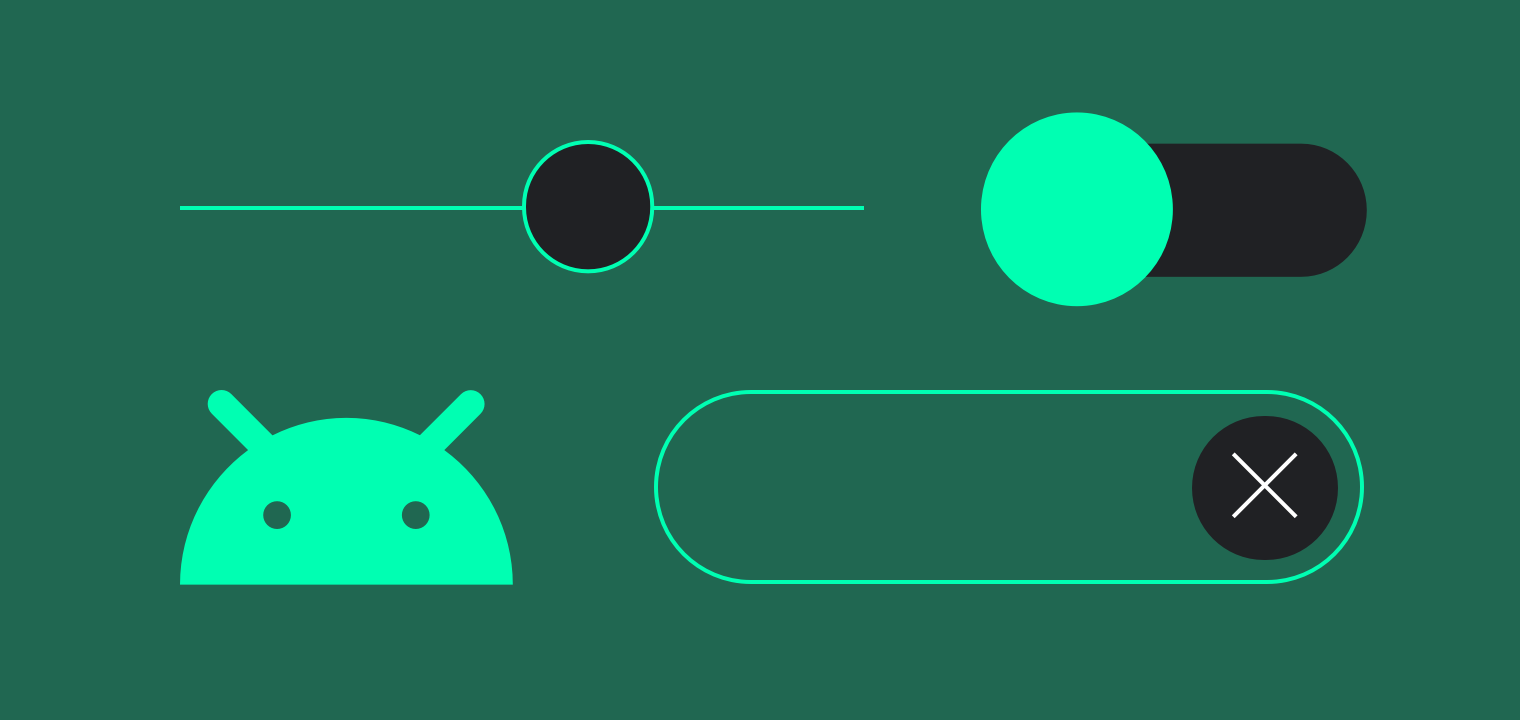
\includegraphics[width=0.6\textwidth]{Bilder/BibliothekenLogos/AndroidMaterialComponenLogo.png}
	\caption{Android Material Components}
\end{figure}


% link: https://material.io/develop/assets/1kvhm0FosmH_nzjOHdtnFX3dQObsxnjv_/android-documents-how-to-components-2x1-large.png

Material Components für Android (MDC-Android) unterstützt Entwickler bei der Ausführung von Material Design. Diese Komponenten wurden von einem Kernteam aus Ingenieuren und UX-Designern bei Google entwickelt und ermöglichen einen zuverlässigen Entwicklungsworkflow zum Erstellen schöner und funktionaler Android-Apps.

Material Components für Android ist ein Ersatz für die Design Support Library von Android.

	\item
	Androidx

\begin{figure}[H]
	\centering
	
\includegraphics[width=0.6\textwidth]{Bilder/BibliothekenLogos/AndroidLogo.png}
	\caption{Androidx Logo}
\end{figure}
	
% link: https://upload.wikimedia.org/wikipedia/commons/thumb/d/d7/Android_robot.svg/1200px-Android_robot.svg.png

Artefakte im Androidx-Namespace umfassen die Android Jetpack-Bibliotheken. Wie die Support-Bibliothek werden Bibliotheken im theandroidx namespace separat von der Android-Plattform geliefert und bieten Abwärtskompatibilität für alle Android-Versionen.

AndroidX ist eine wesentliche Verbesserung gegenüber der ursprünglichen Android-Support-Bibliothek, die nicht mehr gepflegt wird. AndroidX-Pakete ersetzen die Support-Bibliothek vollständig, indem sie Feature-Parität und neue Bibliotheken bereitstellen.

\end{enumerate}


\subsection{Navigationsschema zwischen den Bildschirmen}

Alle Hauptseiten sind durch die Navigation verbunden. Bei jeder Hauptseite befindet sich am Oberen Ende des Bildschirms eine Leiste, in der sich der Name der aktuellen Seite, sowie rechts ein Suchsymbol und  links ein Menüzeichen, mit der sich die Navigation öffnen lässt, befindet. Durch Öffnen der Navigation verlässt man nicht seine aktuelle Seite, sondern sie legt sich von der linken Seite des Geräts über zwei Drittel des Bildschirms und verdunkelt das restliche Drittel leicht. 

Oben in der Navigation ist das Logo der Applikation, ein buntes "Broken Broke Broker", zu sehen. Darunter sind nacheinander die Hauptseiten aufgelistet. Jede Seite hat in seiner Reihe ein zu der Funktion passendes Symbol erhalten und ist erreichbar, indem man auf die genante Reihe drückt. Die Navigation schließt sich, wenn man entweder auf eine der aufgelisteten Seiten oder in das rechte Drittel klickt. Bei ersterem wird zu der Seite navigiert und bei späterem bleibt man einfach auf der aktuellen Seite.

\begin{figure}[H]
	\centering
	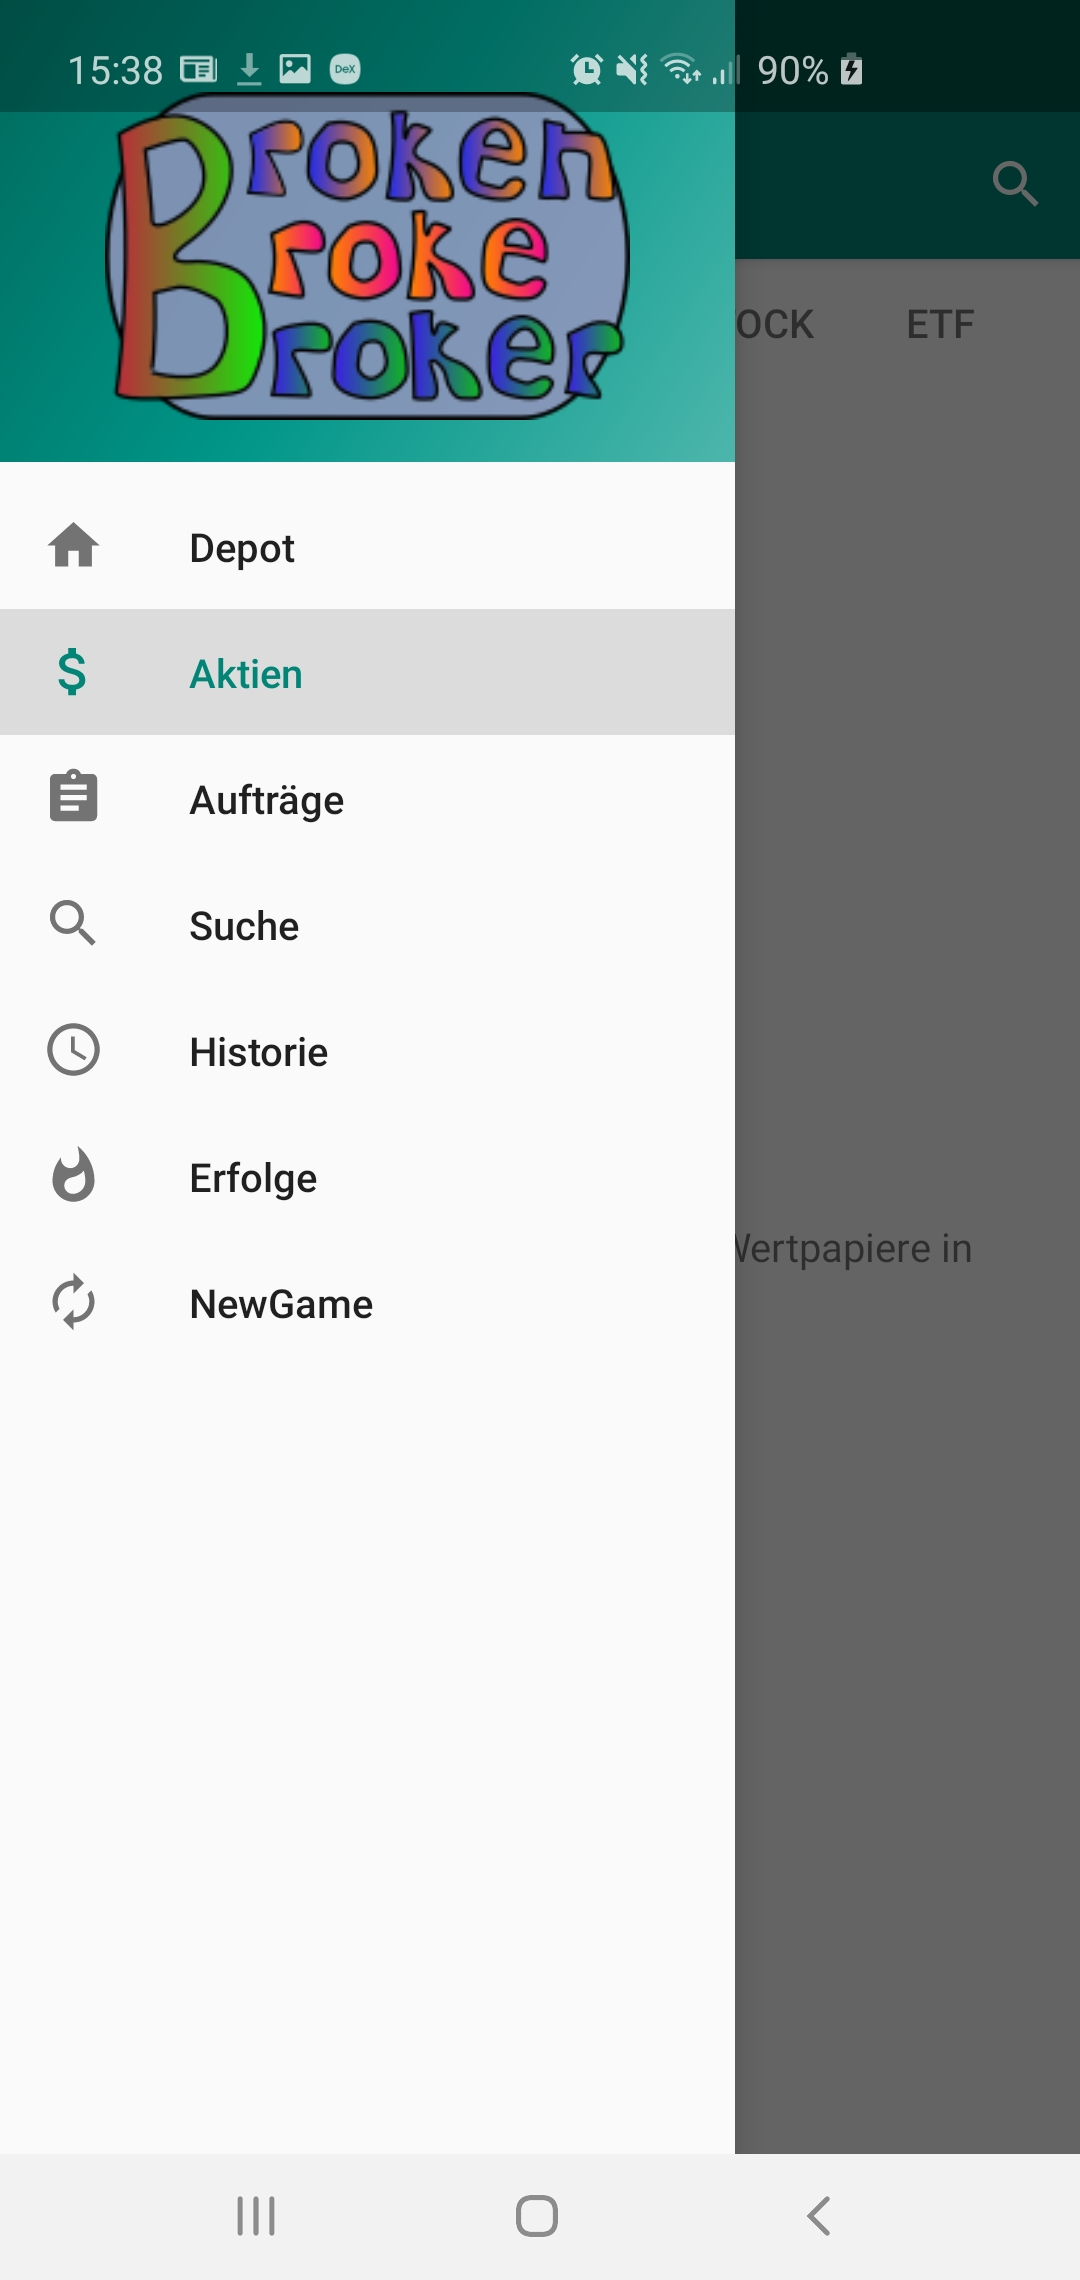
\includegraphics[width=0.6\textwidth]{Bilder/Applikation/Navigation.jpg}
	\caption{Bild der Navigation, die aktuelle Seite ist die, der markierten Reihe}
\end{figure}

\begin{figure}[H]
	\centering
	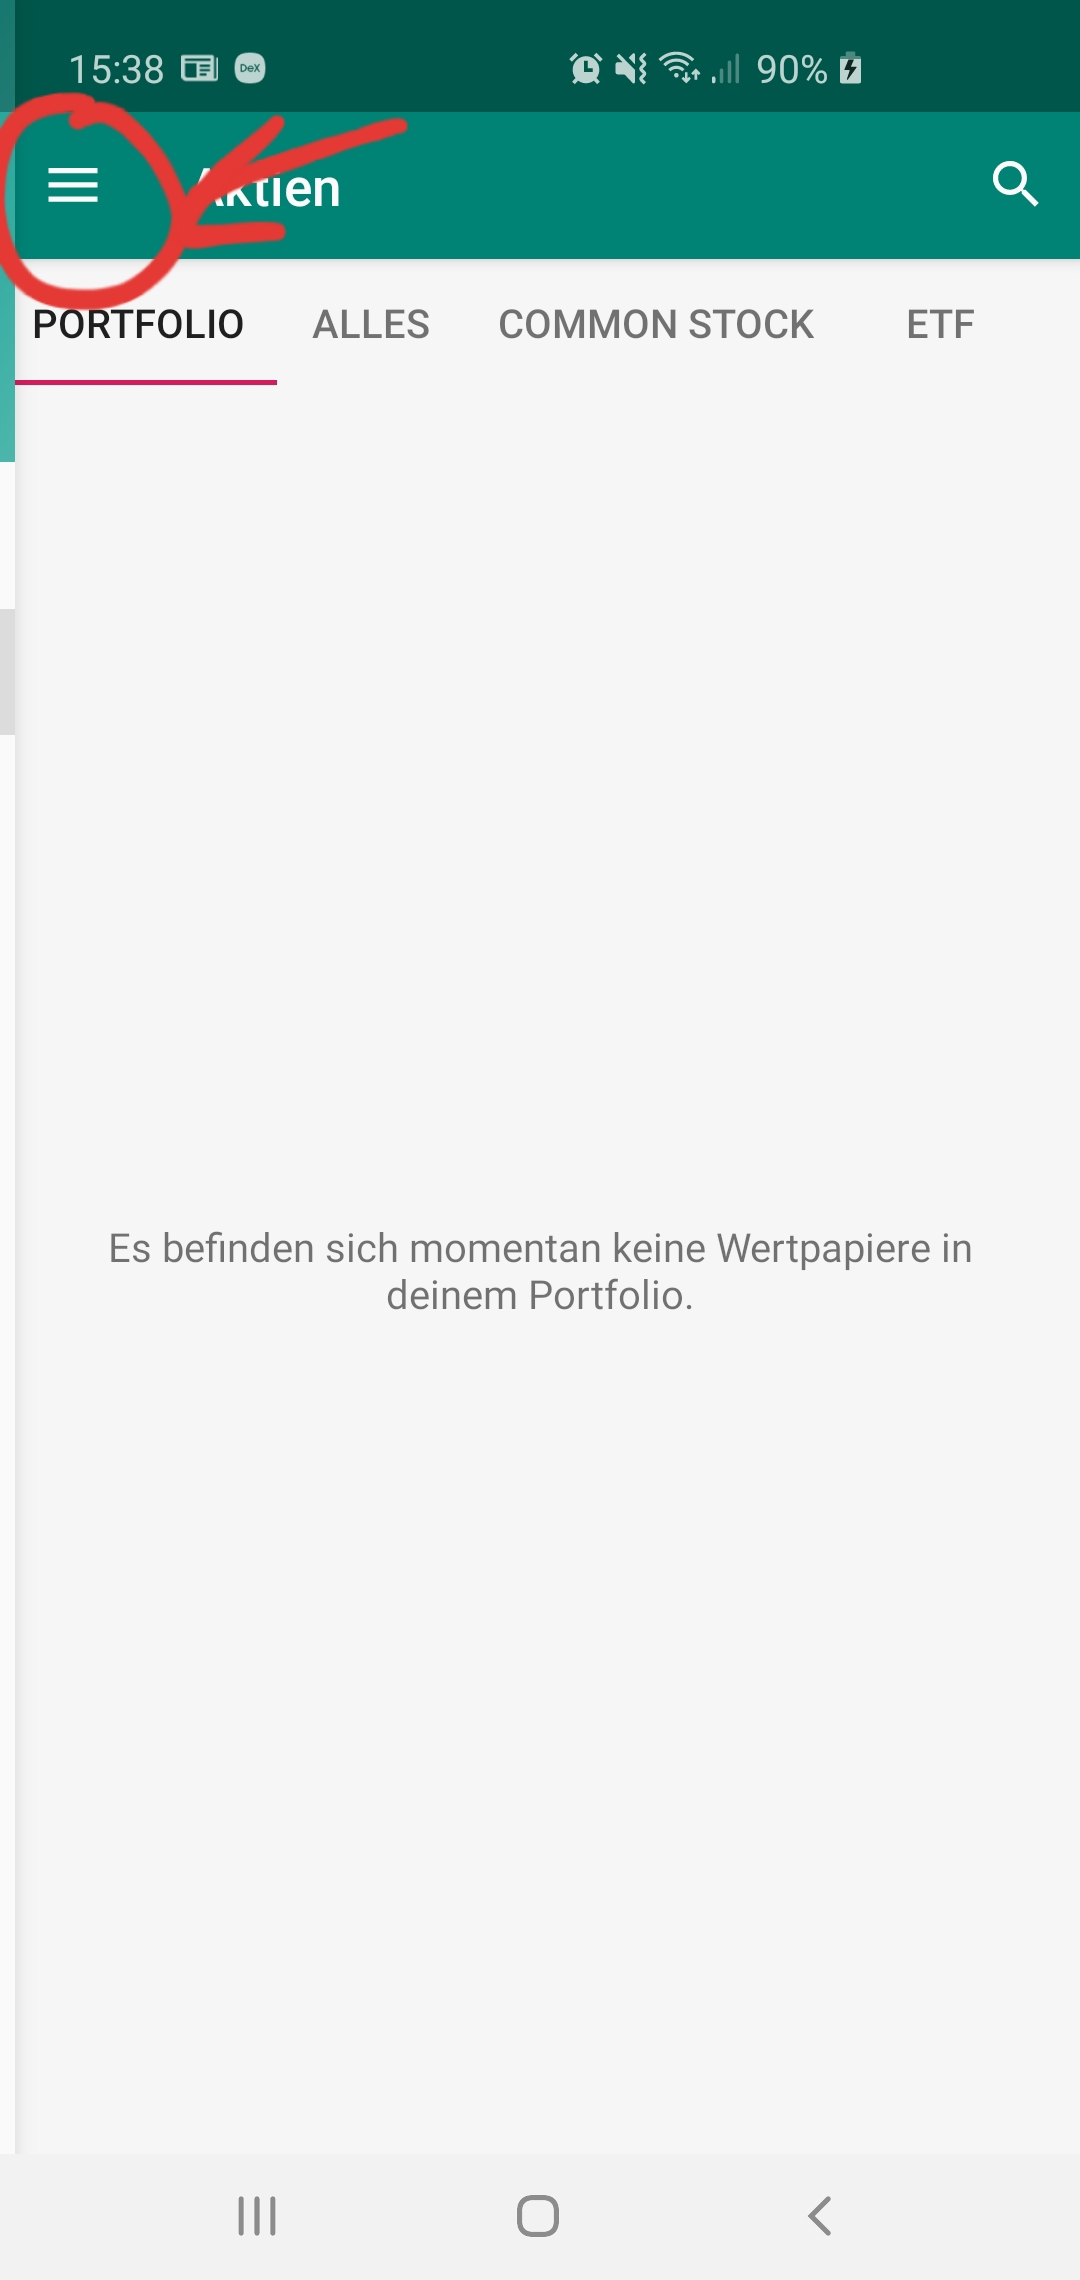
\includegraphics[width=0.6\textwidth]{Bilder/Applikation/NavigationsSymbol.jpg}
	\caption{Bild des Menüzeichens, mit dem sich die Navigation öffnen lässt. Die roten Striche zeigen auf das Symbol}
\end{figure}



\subsubsection{Depot}
Das Depot ist die erste Hauptseite und auch die Startseite. Nach dem Öffnen der Applikation gelangt man immer zu erst in der Depot, da sich das Spiel auch größtenteils um dessen Inhalt dreht. Dort werden nämlich die Hauptressourcen, die eigenen Aktion, verwaltet.

Das Depot ist eingeteilt in Übersicht und Statistik. Beide Punkte befinden sich nebeneinander direkt unterhalb der Leiste, die zur Navigation gehört. Der ausgewählte Punkt ist rot unterstrichen und beeinflusst den darunterliegenden Teil der Seite. Beim Start gelangt man immer zu Erst in die Übersicht aber wenn man sich beim letzten Verlassen der Seite in der Statistik befand, dann gelangt man beim nächsten Besuch auch zu erst in die Statistik.

Die Übersicht beinhaltet als erstes den aktuellen Kontostand, sowie den gesamten Wert der Wertpapiere und die daraus resultierende Summe. Darunter sind dann die im Besitz befindenden Aktien aufgelistet. Geht die Liste nach unten hin über den Rand des Bildschirm hinaus, kann man die unteren Teile durch scrollen erreichen. Die oberen Listeneinträge werden dann durch die unteren ersetzt aber alles oberhalb der Liste bleibt unverändert.
Jede anklickbare Aktie in allen Menüs hat immer die gleiche rechteckige Form. Auch die Anordnung der Daten ist immer gleich. Links oben steht das Symbol(Abkürzung) der Aktie. Darunter ist dann der Name der Firma, wenn man die Aktie vorher einmal geladen hat. Rechts unten steht die Abkürzung des Types, wie zum Beispiel "cs" für "Common Stock" Darüber steht, falls man solche Aktien besitzt, die Anzahl und der aktuelle Preis.

Kryptowährungen haben die gleiche Form wie Aktien in der Anzeige. Sie unterscheiden sich nur in der Detailansicht, wenn man darauf klickt.

	
\todo{Bilder von Depot(Übersicht) einfügen}


\todo{Statistik, wenn fertig}

\subsubsection{Aktien}
Die Aktiendetailansicht lässt sich von überall erreichen, wo sich Aktien in einer Liste befinden. Diese kann man anklicken und wird zu ihrer Detailansicht weitergeleitet. In dieser Detailansicht werden genauere Informationen über die Aktie dargestellt. Man kommt zurück zur letzten Stelle, indem man oben links auf den Pfeil klickt.

Ganz oben in der Ansicht steht der Firmennahme der Aktie. Direkt darunter wird ein Graph geladen, der die Range des Preises für jeden Tag des letzten Monats anzeigt. Über dem Graphen steht das aktuelle Datum (Amerikanisch) und der Titel des Graphen mit den höchsten und niedrigsten dargestellten Werten dahinter. 

Unter dem Graphen befinden sich zwei Blöcke mit Informationen. Als erstes die Daten zu dem Symbol, dem Firmennamen, der Kategorie und der aktuelle Preis der Aktie. Danach noch der letzte Schließpreis, das Datum des letzten Höchstpreises und das 52-Wochen hoch bzw. tief.
Dann folgen zwei Knöpfe mit den Optionen Kaufen und die Aktie zum Portfolio hinzufügen.

Durch Druck auf den unteren Knopf fügt man die Aktie zum Portfolio hinzu und der Knopf ändert seine Schrift zu "Aus dem Portfolio entfernen". Der Knopf bekommt dann auch die gleiche Funktion.

Drückt man auf den vorderen Knopf, öffnet sich ein "Aktie kaufen" Popover, in dem zu erst das eigene Vermögen und der Stückpreis der Aktie stehen. Es folgen zwei Nummernfelder für die Kaufmenge und das Limit, dann der Gesamtwert der Stückzahl, gefolgt von einem "Verwerfen" und einem "Kaufen" Knopf. Mit "Verwerfen" schließt sich das Popover und es wird keine weitere Aktien ausgeführt. Durch "Kaufen" kauft man die Aktien, vorausgesetzt, man hat die Stückzahl angegeben und genug Geld. Bei Limit kann man den Preis angeben, den man bereit wäre für diese Aktie zu bezahlen. Tut man dies, und bestätigt man, indem man auf "Kaufen" klickt, so wird ein Kaufauftrag erstellt und die Applikation kauft für den Nutzer automatisch die gewünschte Anzahl der Aktie, wenn das Limit unterschritten wird. Der Kaufauftrag wird danach in der dazugehörigen Hauptseite aufgelistet. Hat man einen Kaufauftrag erstellt, wird dieser unter dem Portfolio Knopf aufgelistet und ein weiterer Knopf erscheint, mit dem man alle Aufträge löschen kann.

Besitzt man Teile der ausgewählten Aktie, taucht der Knopf "Verkaufen" zwischen den beiden ursprünglichen auf. Drückt man darauf, öffnet sich ein Popover, genau wie bei "Kaufen". Der Inhalt ist auch gleich, nur jedes "Kaufen" ist durch "Verkaufen" ersetzt. In dem Fenster kann man seine Aktien verkaufen oder einen Verkaufsauftrag erstellen, der vom Prinzip wie der Kaufauftrag funktioniert. Wird das Limit in dem Fall überschritten, verkauft die Applikation automatisch die gewünscht Stückzahl der ausgewählten Aktie und listet den Auftrag in der Detailansicht und auf der Hauptseite Aufträge auf.

\begin{figure}[H]
	\centering
	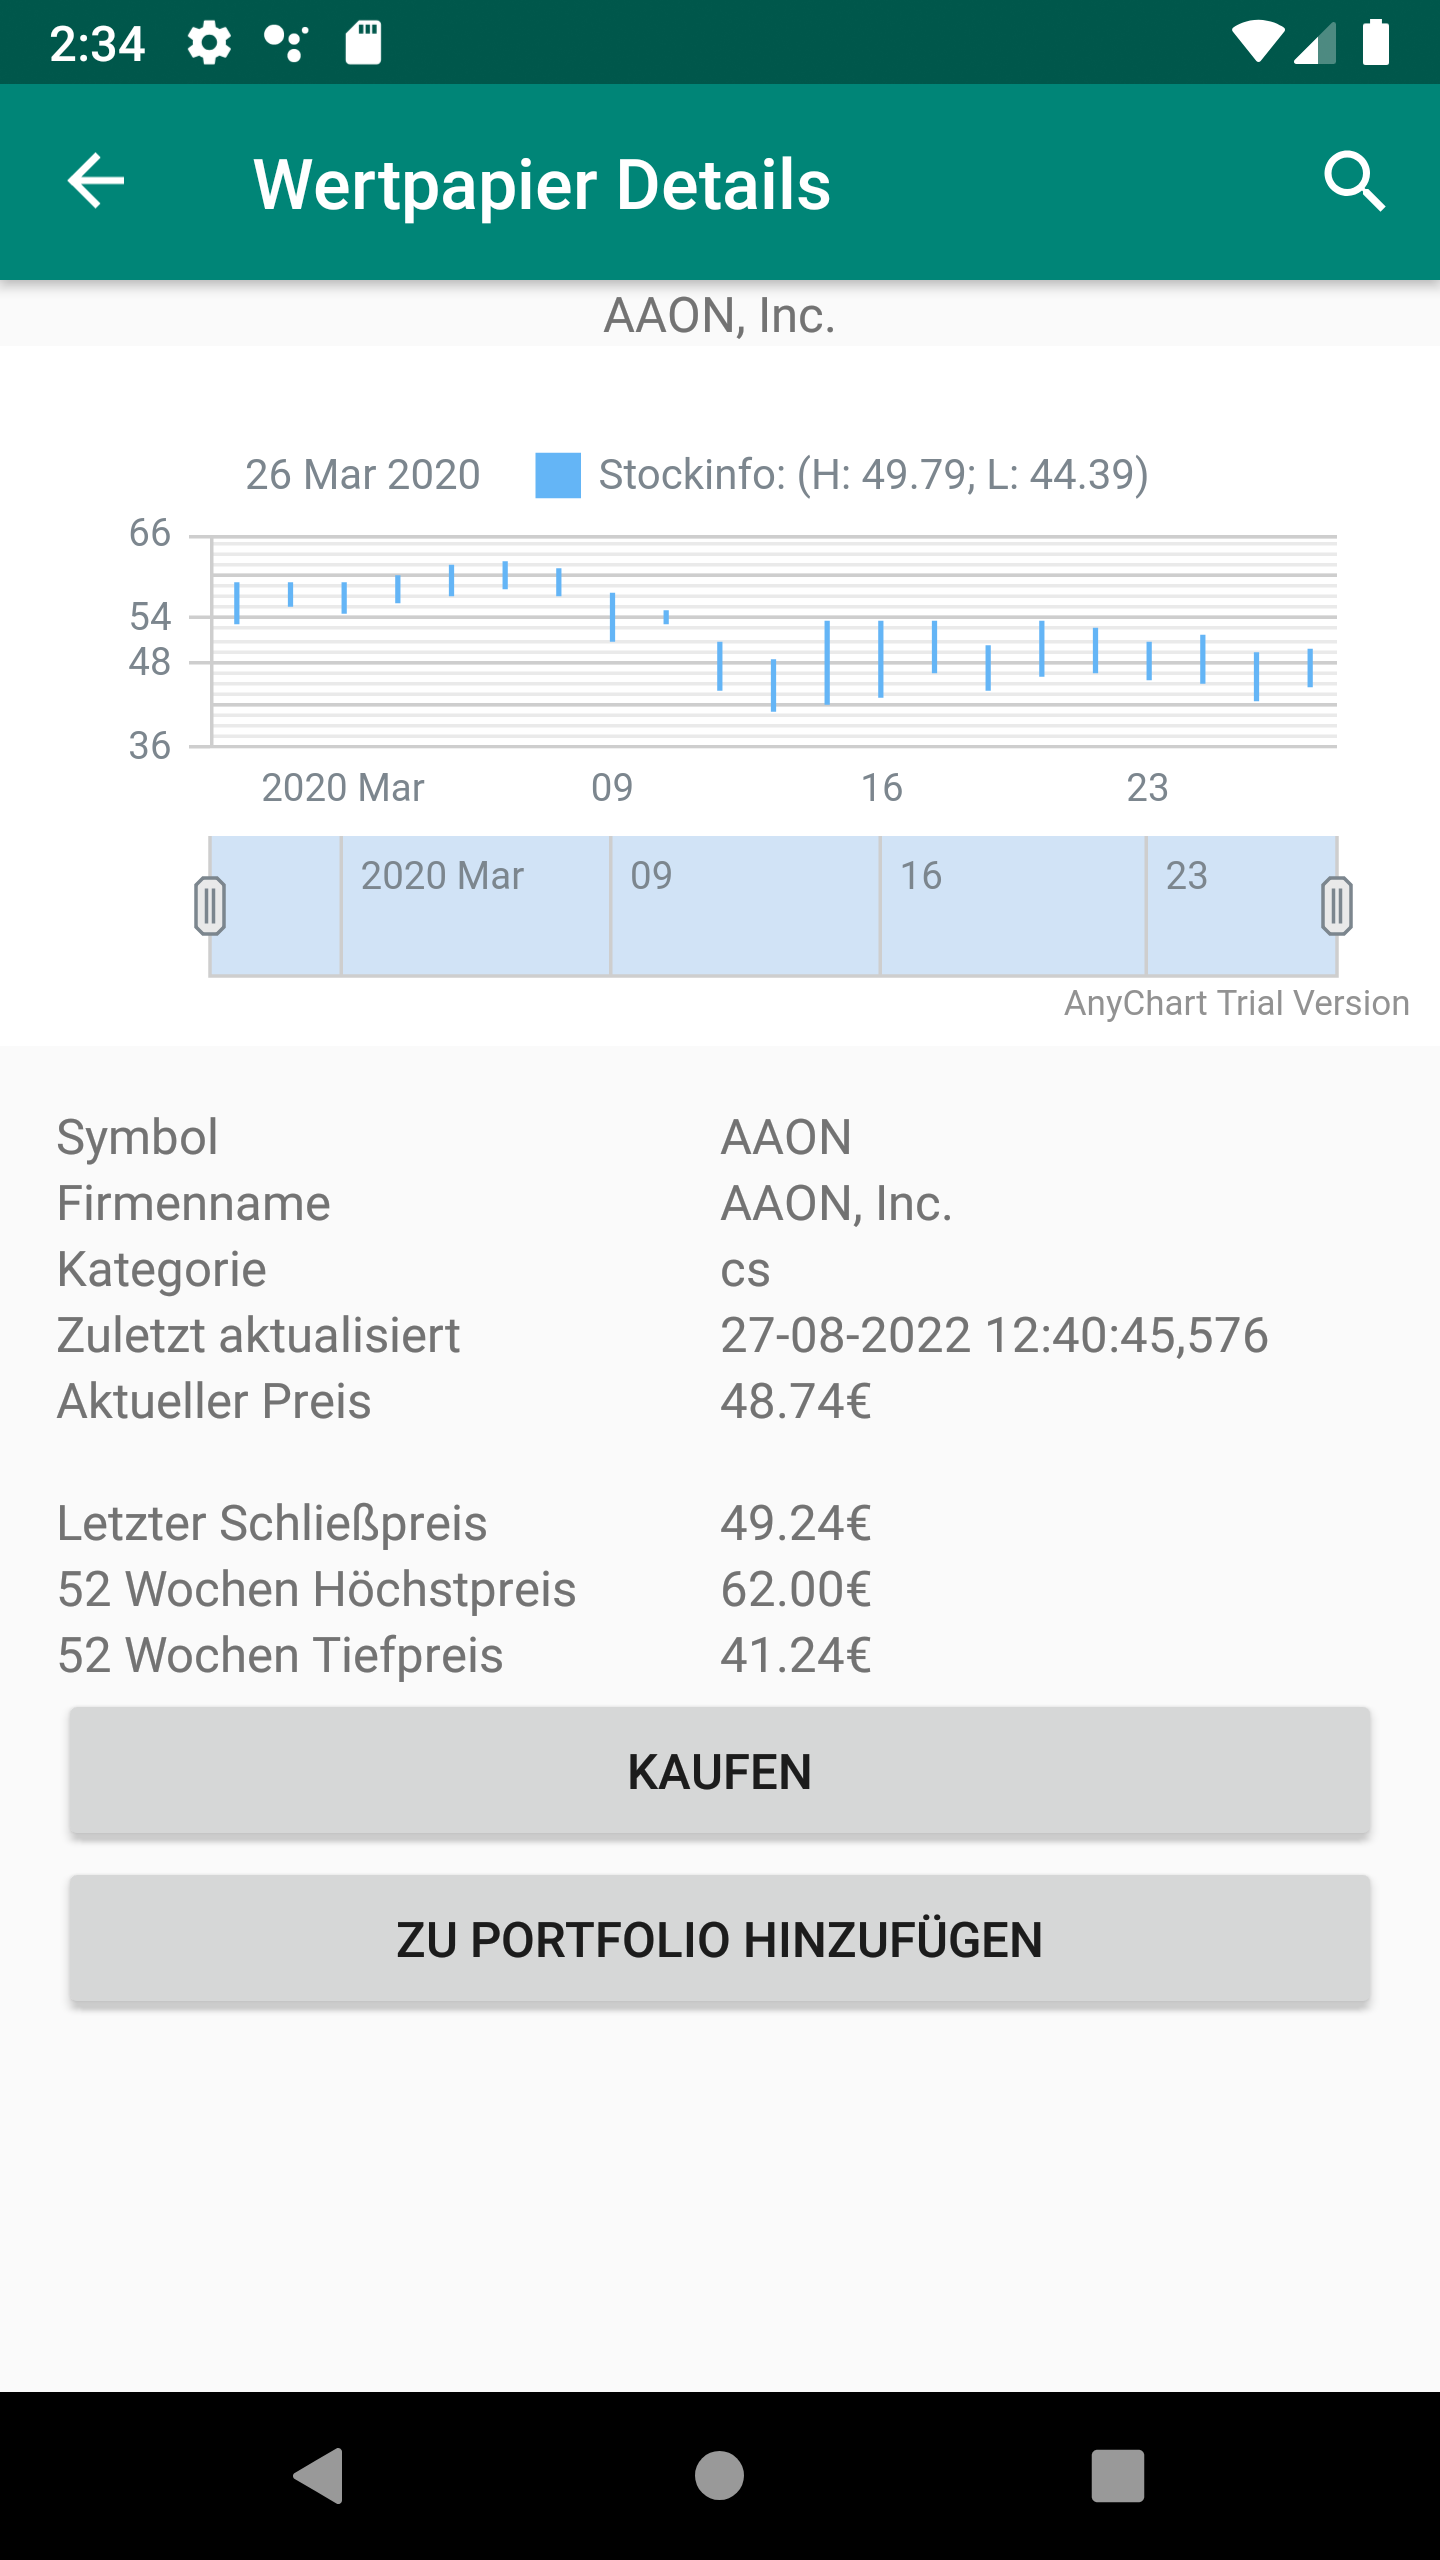
\includegraphics[width=0.6\textwidth]{Bilder/Applikation/AktienDetails.png}
	\caption{Aktiendetailansicht ohne Einflüsse}
\end{figure}

\begin{figure}[H]
	\centering
	\includegraphics[width=0.6\textwidth]{Bilder/Applikation/AktienDetailsAufträge.png}
	\caption{Aktiendetailansicht mit Aufträgen und Aktien im Besitz}
\end{figure}

\begin{figure}[H]
	\centering
	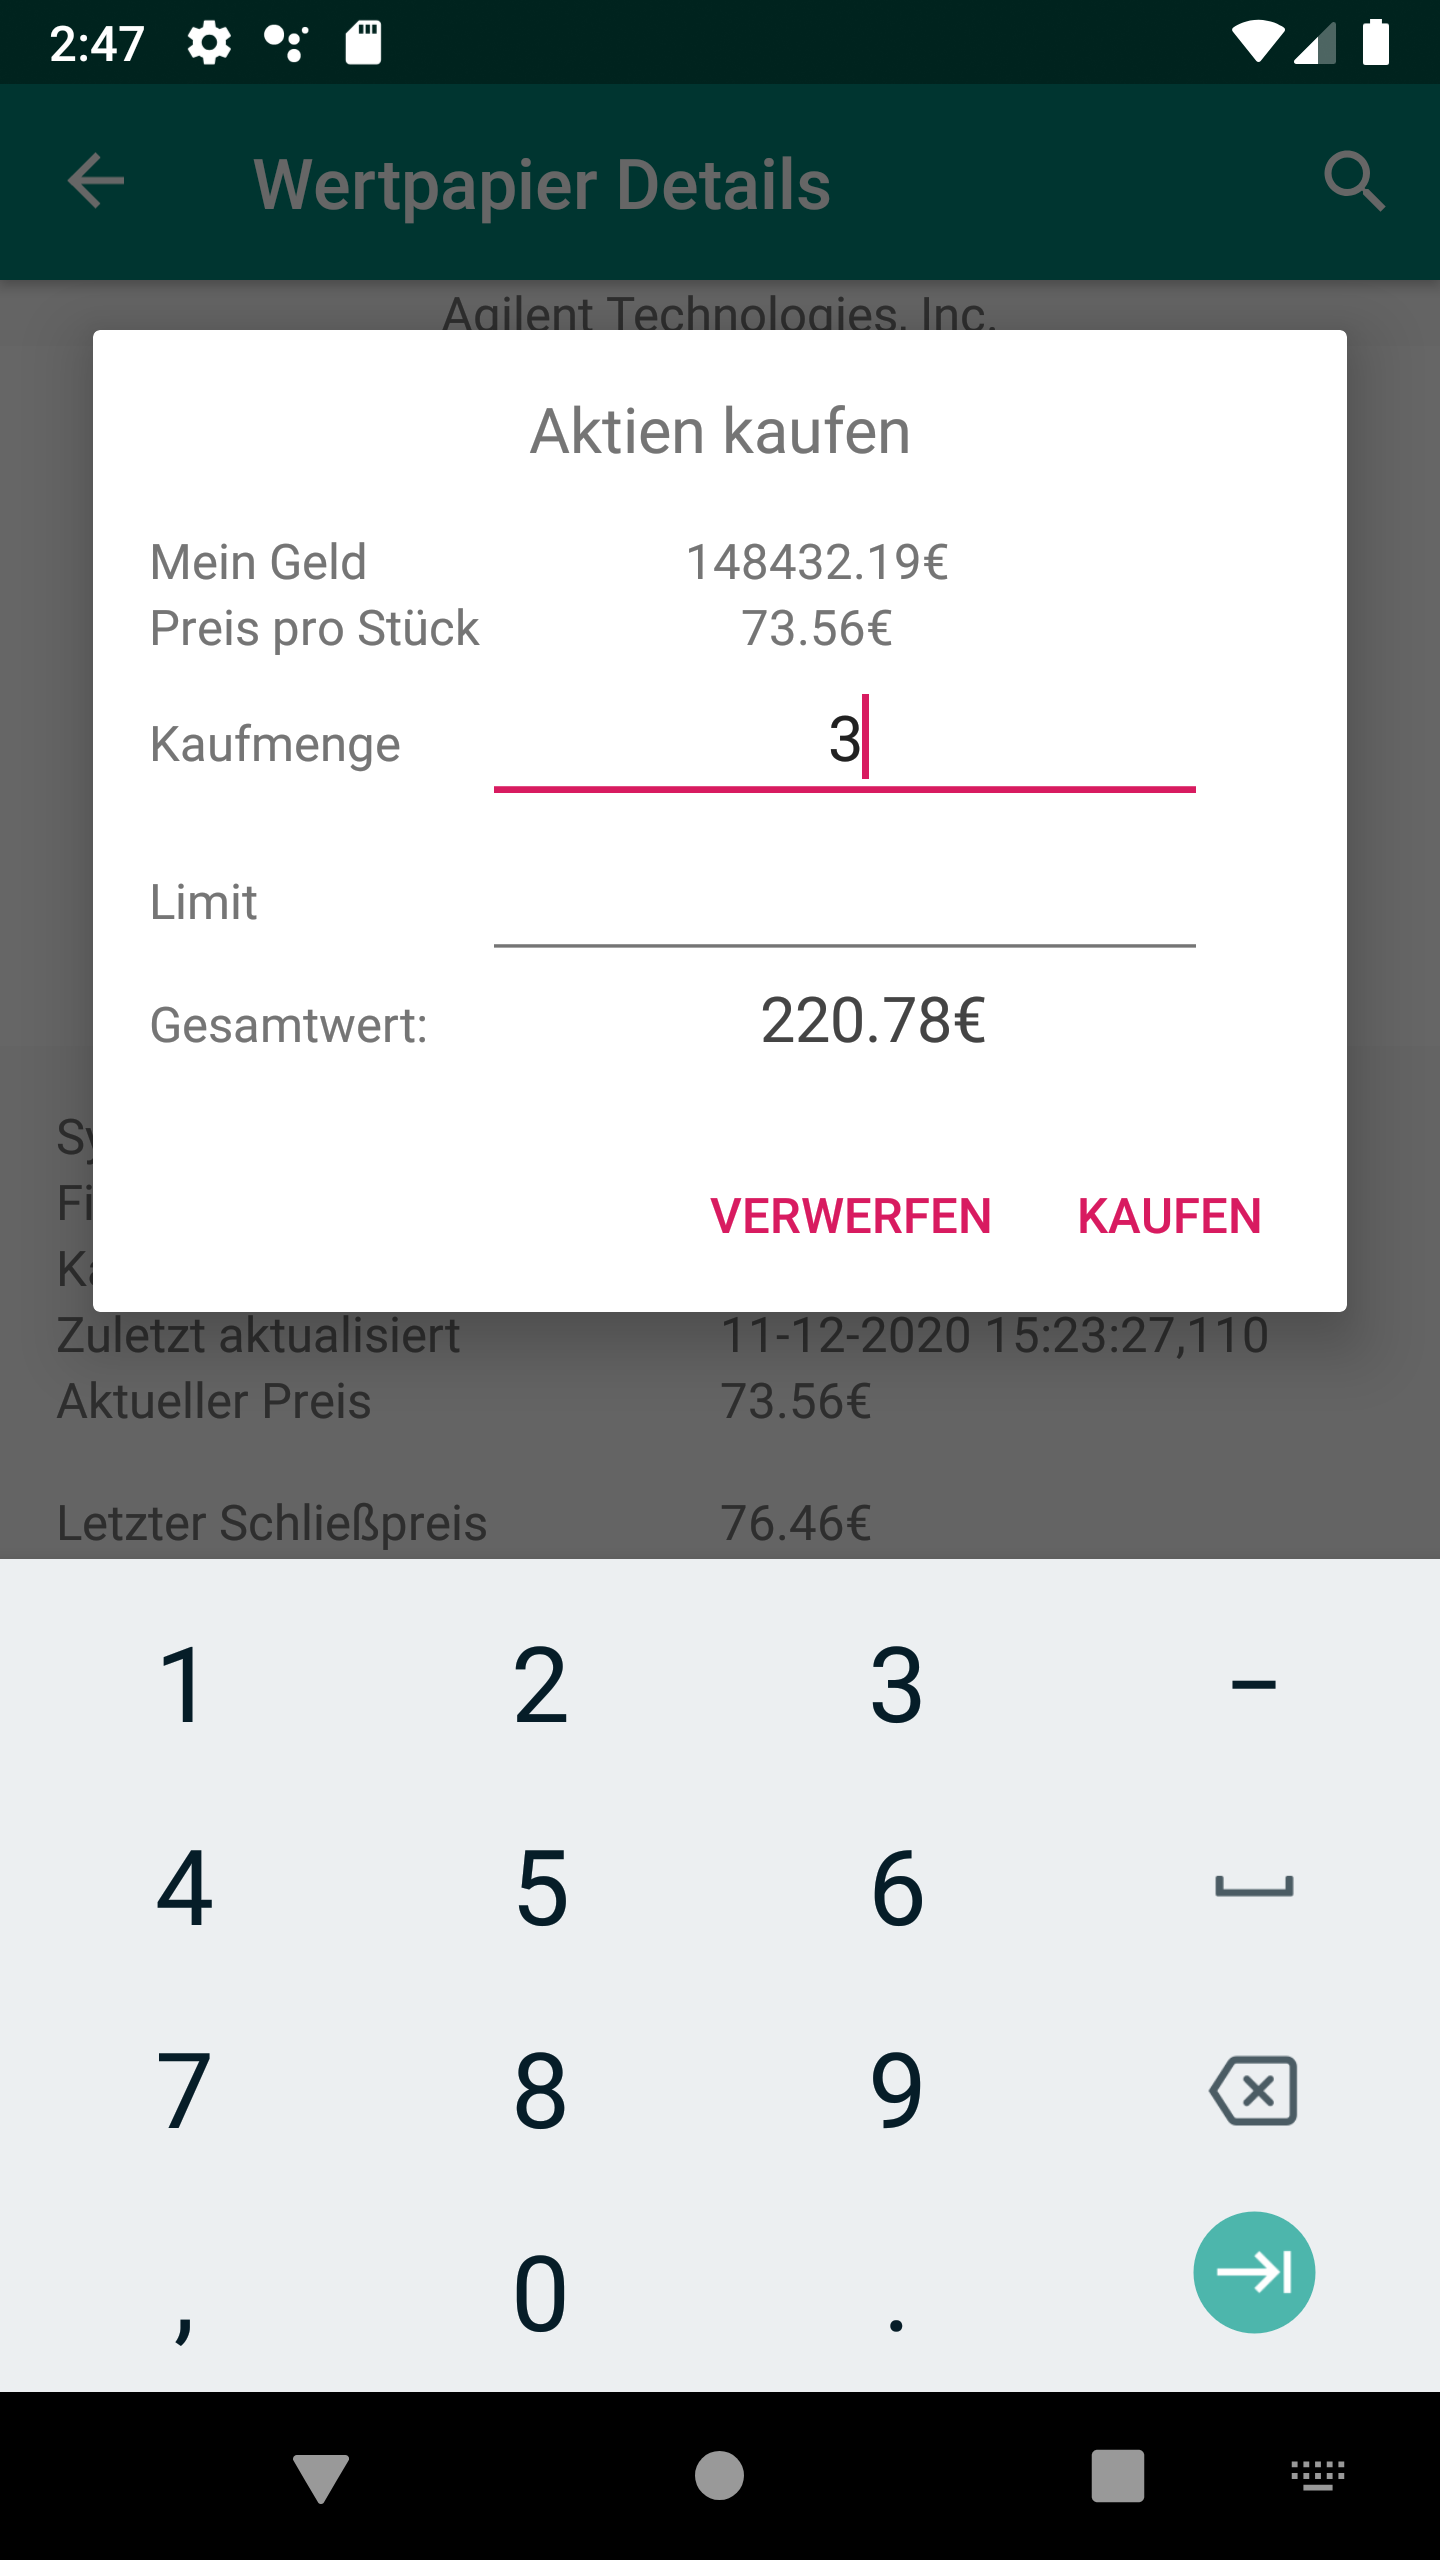
\includegraphics[width=0.6\textwidth]{Bilder/Applikation/AktieKaufen.png}
	\caption{Aktie kaufen Ansicht}
\end{figure}

\begin{figure}[H]
	\centering
	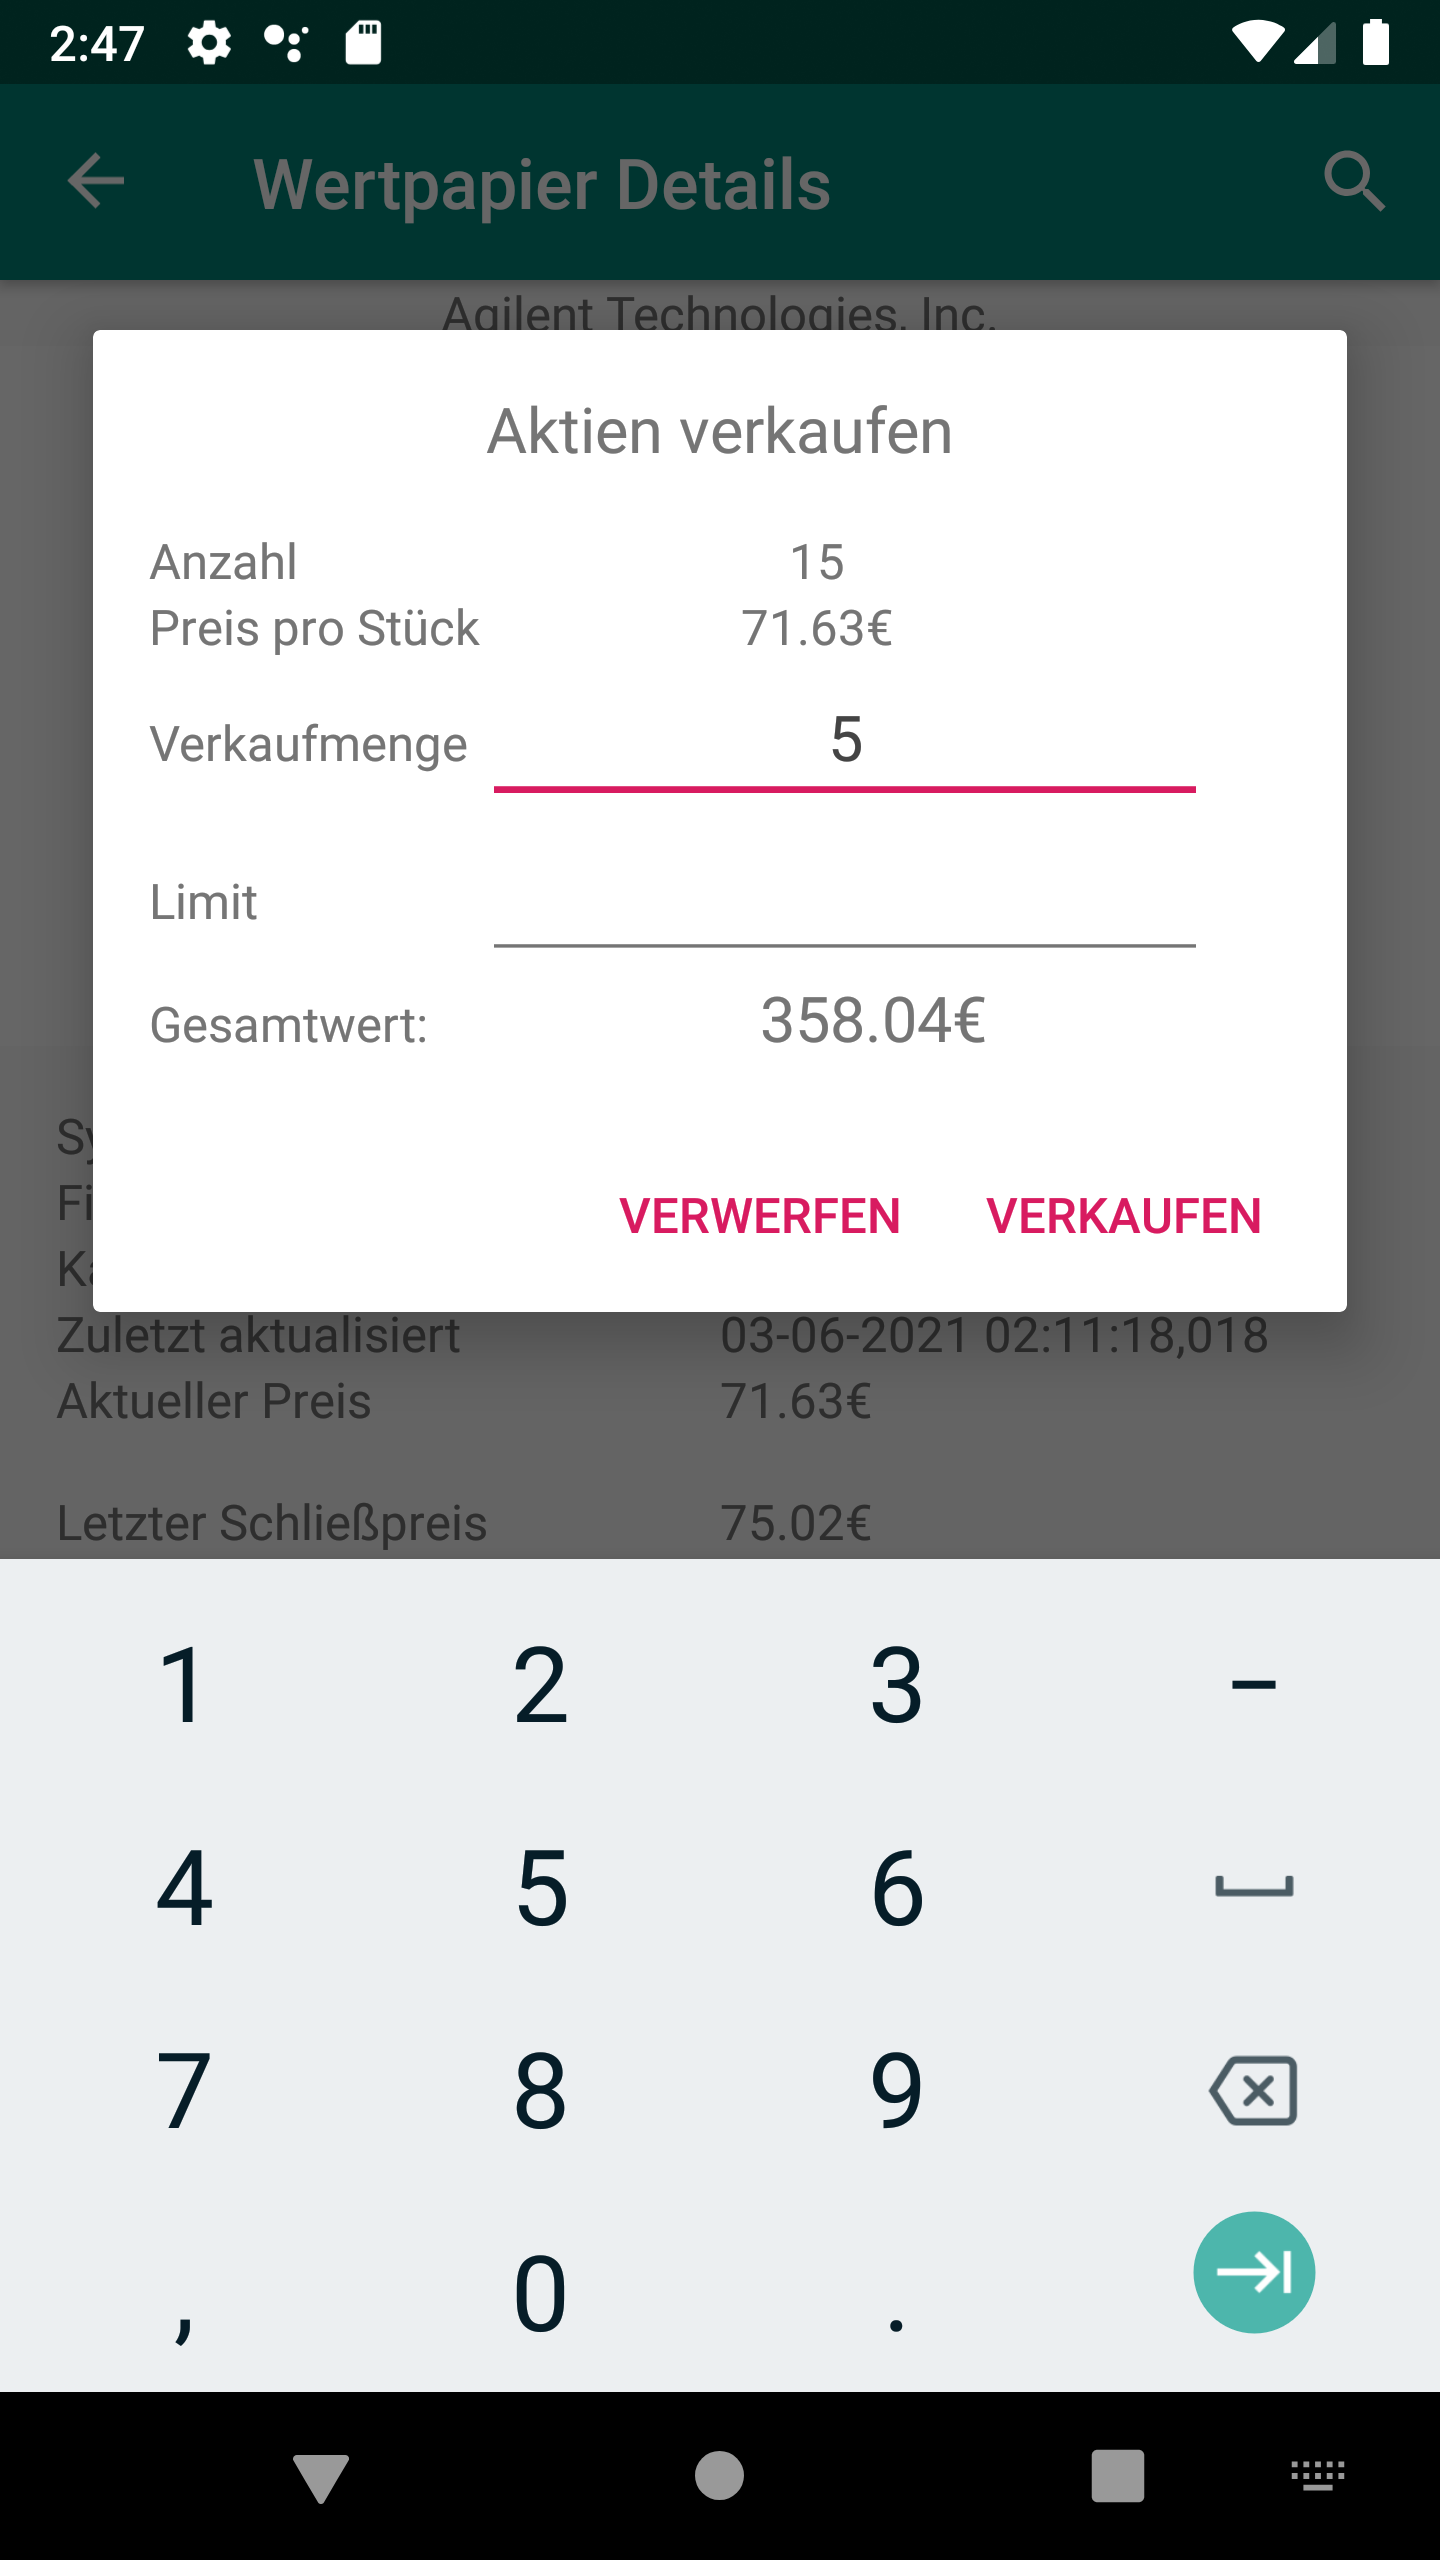
\includegraphics[width=0.6\textwidth]{Bilder/Applikation/AktieVerkaufen.png}
	\caption{Aktie verkaufen}
\end{figure}

\subsubsection{Aktien}
Wenn man das erste mal zu dieser Seite navigiert wird, gelangt man zu seinem Portfolio. Darin sind alle Aktien zu sehen, die man vorher zu dem Portfolio hinzugefügt hat. Es dient als eine Übersicht für die besonders interessanten Aktien, die man im Auge behalten möchte. Ähnlich wie bei Übersicht und Statistik im Depot befindet sich direkt unter der Navigationsleiste Wahlmöglichkeiten, die die Seite darunter verändern. Neben dem Portfolio gibt es dort die Möglichkeit auf "Kryptowährungen" zu klicken, doch werden alle Kryptowährungen angezeigt. Direkt daneben steht "Aktien" die eine Übersicht über alle verfügbaren Aktion liefert. Die Leiste mit diesen Wahlmöglichkeiten lässt sich nach rechts scrollen, indem man die Leiste nach links zieht. Die weiteren Sektionen enthalten Teile von allen verfügbaren Aktien, die kategorisch zusammengefasst sind. Die Leiste enthält jedoch nicht alle möglichen Kategorien sondern nur diese, die auch Aktien enthalten. Die Liste wird regelmäßig geupdated, also ist es möglich, dass einige Kategorien aus der Leiste verschwinden oder hinzugefügt werden.

Durch klick auf eine bestimmte Aktie gelangt man zu der dazugehörigen Aktiendetailansicht. Der Knopf, der zur Navigation führt wird dann durch einen Pfeil ersetzt, der zurück zu der vorherigen Stelle in der Liste der Aktien führt.

\begin{figure}[H]
	\centering
	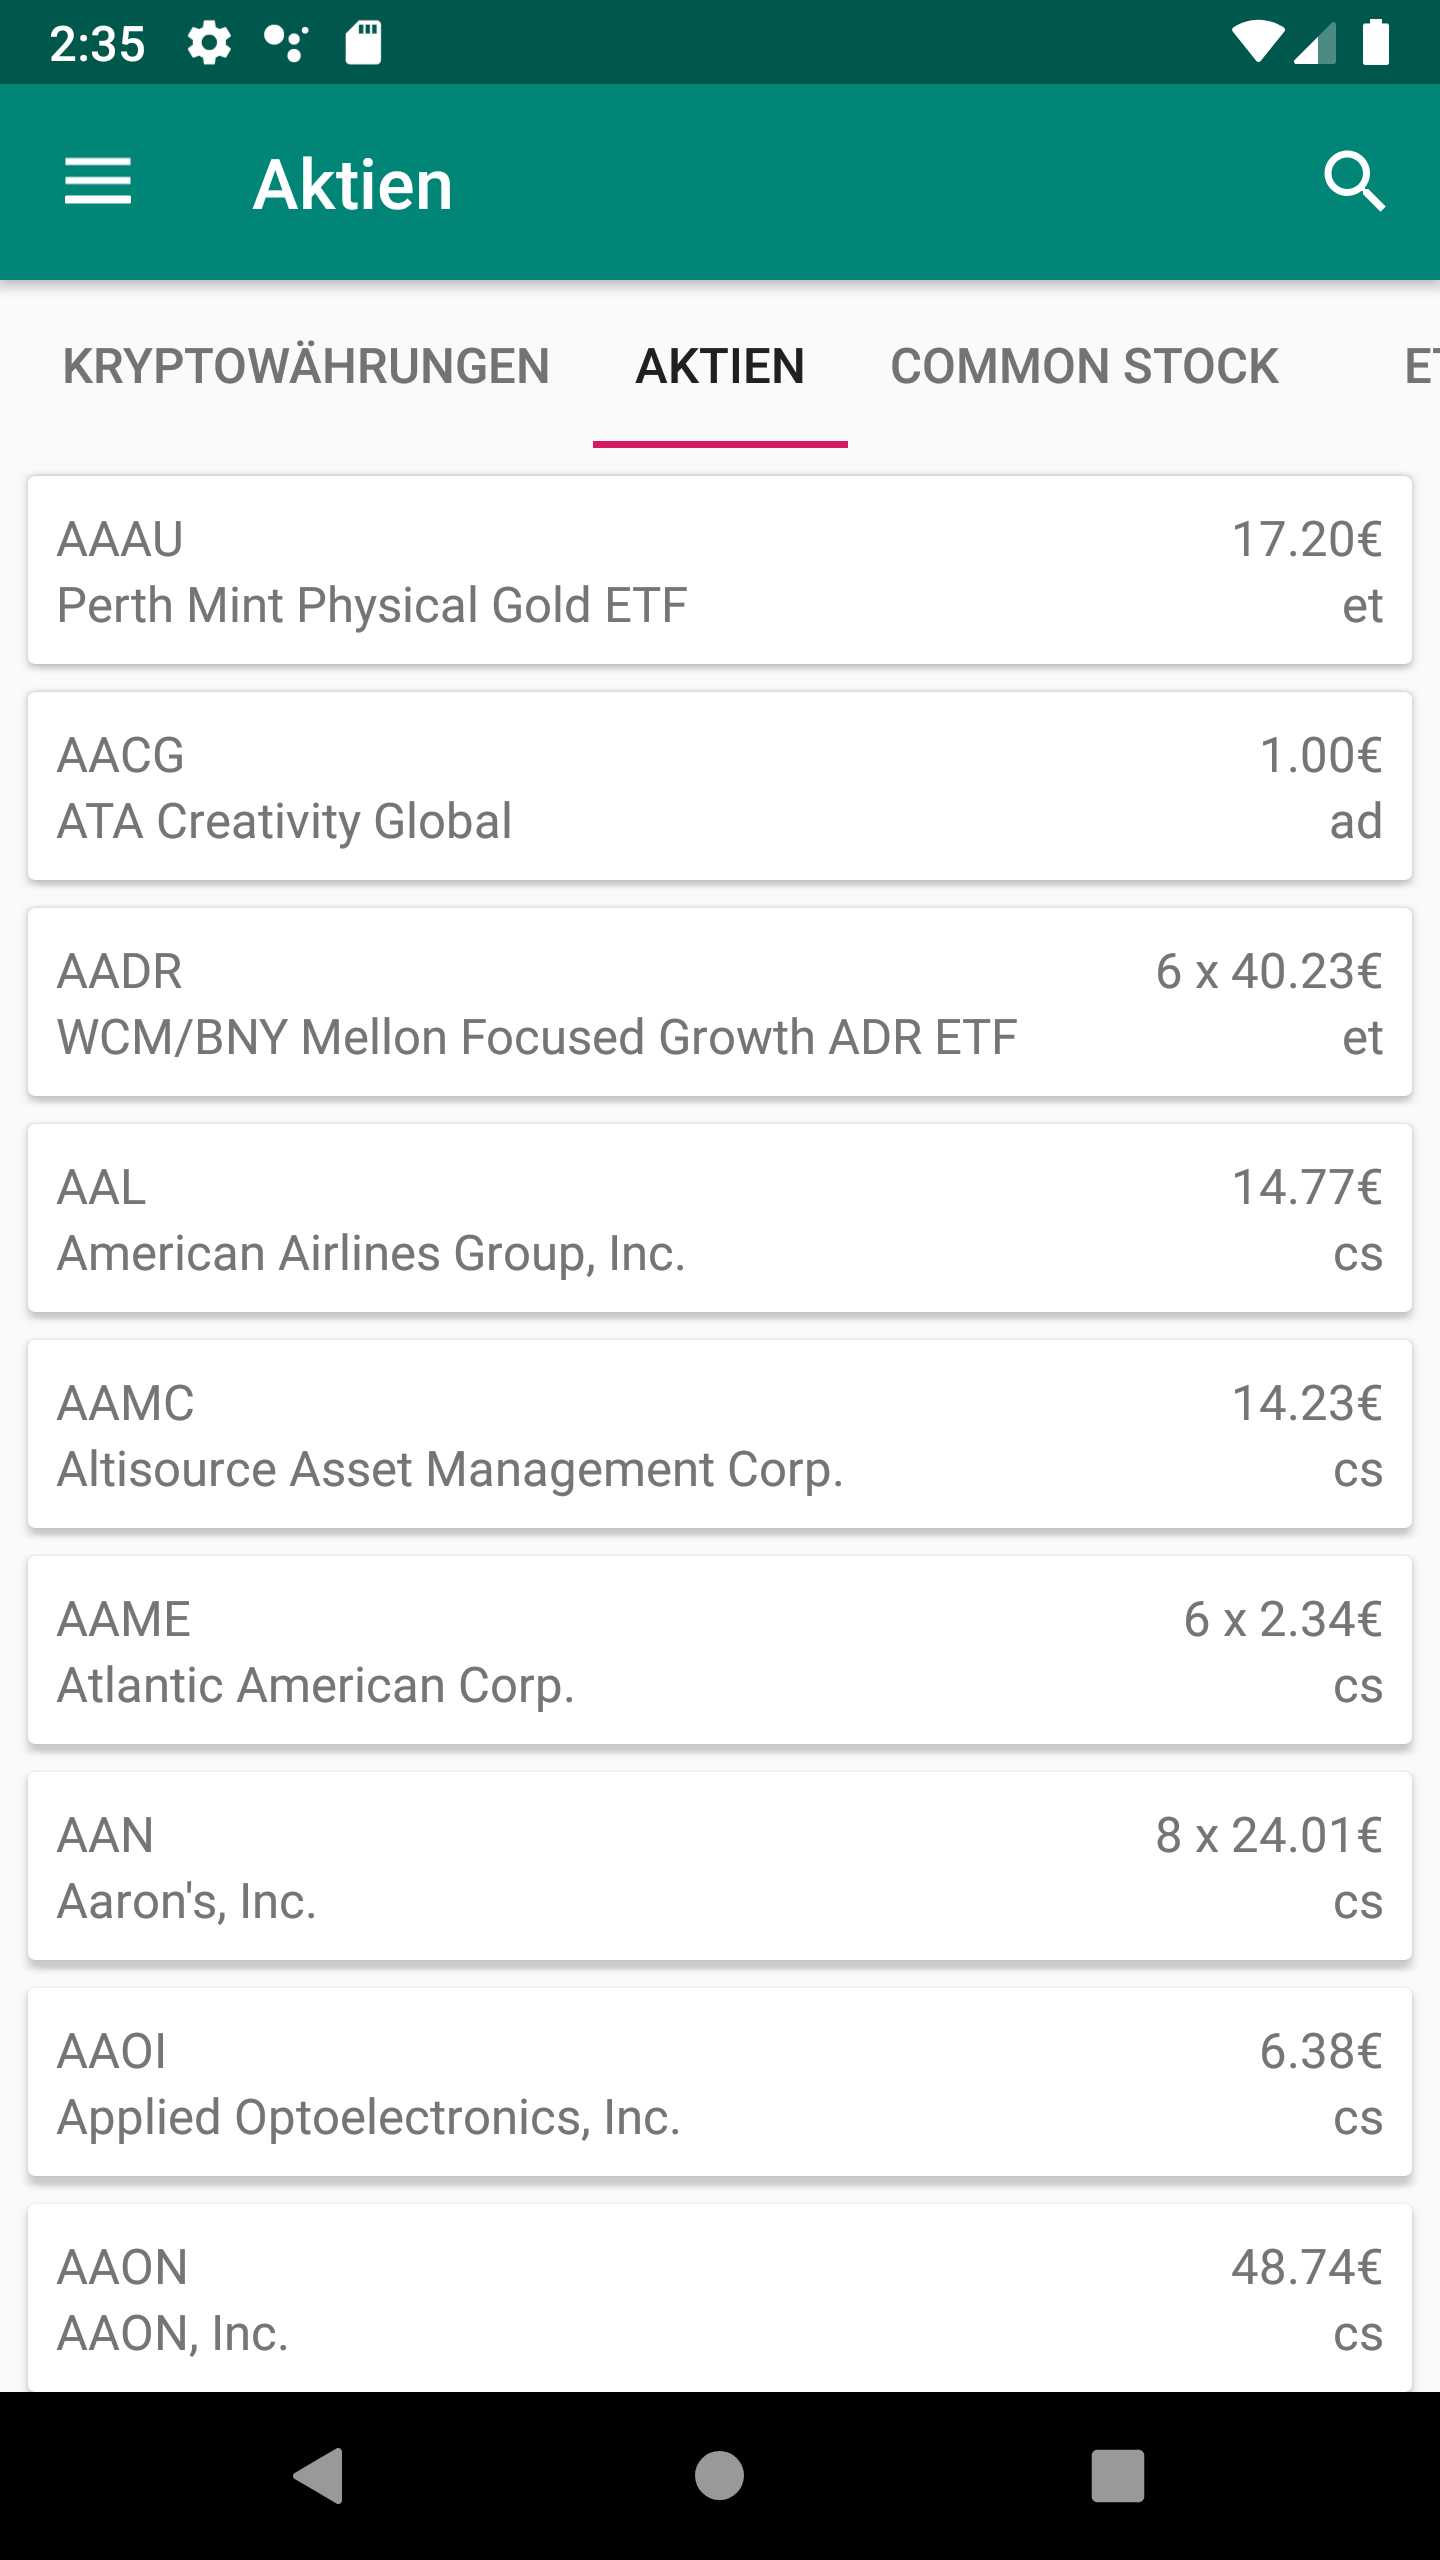
\includegraphics[width=0.6\textwidth]{Bilder/Applikation/Aktien.png}
	\caption{Aktienansicht}
\end{figure}

\subsubsection{Kryptowährungendetailansicht}

Kryptowährungen sehen in den Listen genau aus wie Aktien. Als Kategorie steht dort "crypto". Klickt man auf sie, wird man jedoch nicht zu der Üblichen Aktiendetailansicht weitergeleitet, sondern zu einer etwas anders aussehenden Kryptowährungendetailansicht.

In dieser Detailansicht ist oben ein Graph, der den Preisverlauf der Währung darstellt- Dieser Graph wird allerdings nur bei Kryptowährungen angezeigt, die mehr als ein Cent wert sind. Unter dem Graphen befindet sich ein Informationblock mit dem Symbol, der Kategorie, dem Zeitpunkt der letzten Aktualisierung und dem aktuellen Preis.

Darunter befinden sich noch Knöpfe mit den gleichen Funktionen wie in der Aktiendetailansicht. Auch Kaufen und Verkaufen ist genau gleich.

\begin{figure}[H]
	\centering
	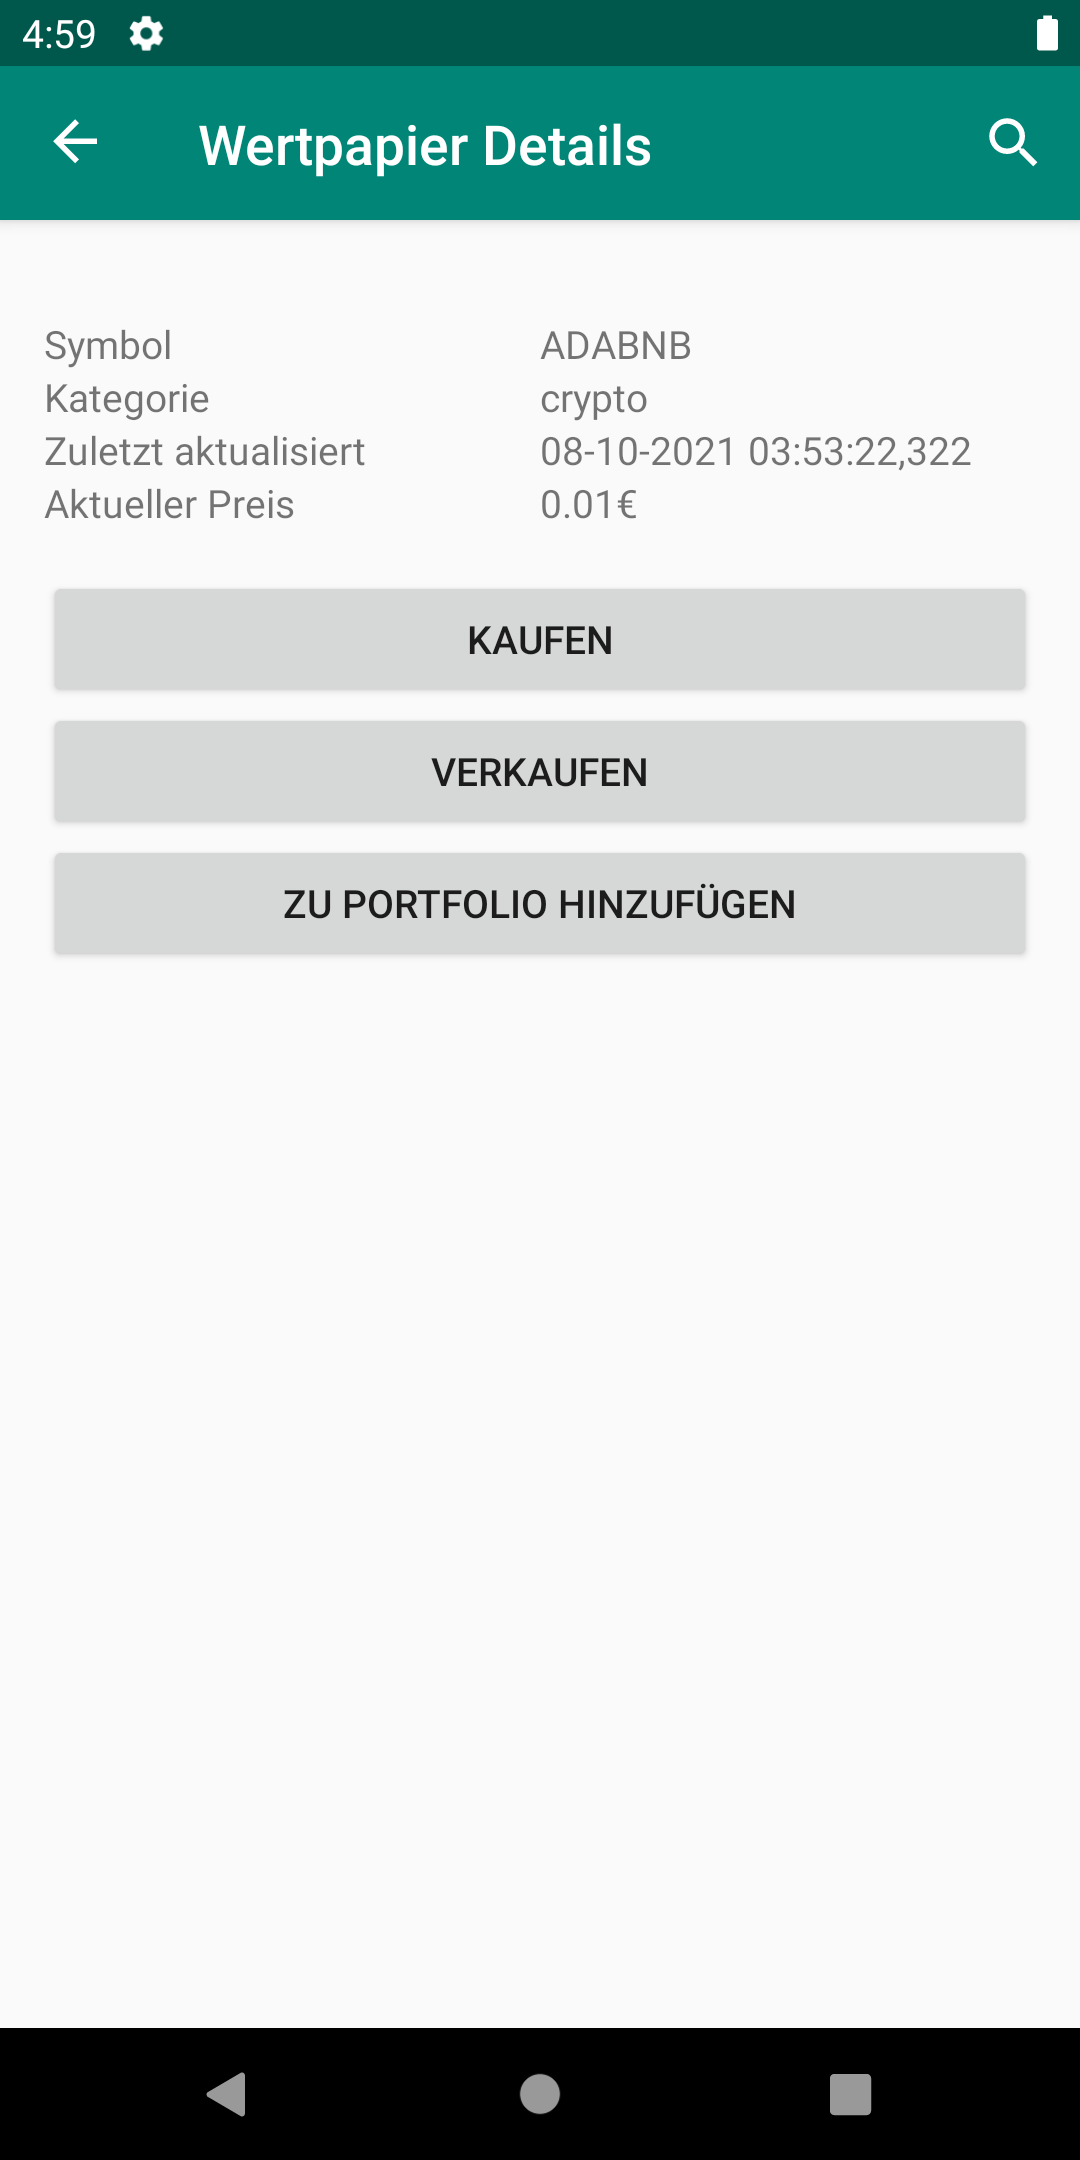
\includegraphics[width=0.6\textwidth]{Bilder/Applikation/krypto.png}
	\caption{Kryptowährungendetailansicht}
\end{figure}

\subsubsection{Aufträge}

Aufträge sind auch wieder in zwei Sektionen aufgeteilt. In Kaufaufträge und Verkaufsaufträge. Unter jeder Sektion befindet sich eine Liste mit den Aktien, für die die Aufträge bestehen. Dort wo sonst der aktuelle Preis der Aktie steht, befindet sich nun die Anzahl des Auftrags und dahinter der Preis, für den die Aktien gekauft werden sollen. Bei den Verkaufsaufträgen sieht es ähnlich aus, nur das hier die Preis, für den die Aktien verkauft werden sollen, steht.

Klickt man auf die Aktie in der Liste gelangt man in ihre Detailansicht.

\begin{figure}[H]
	\centering
	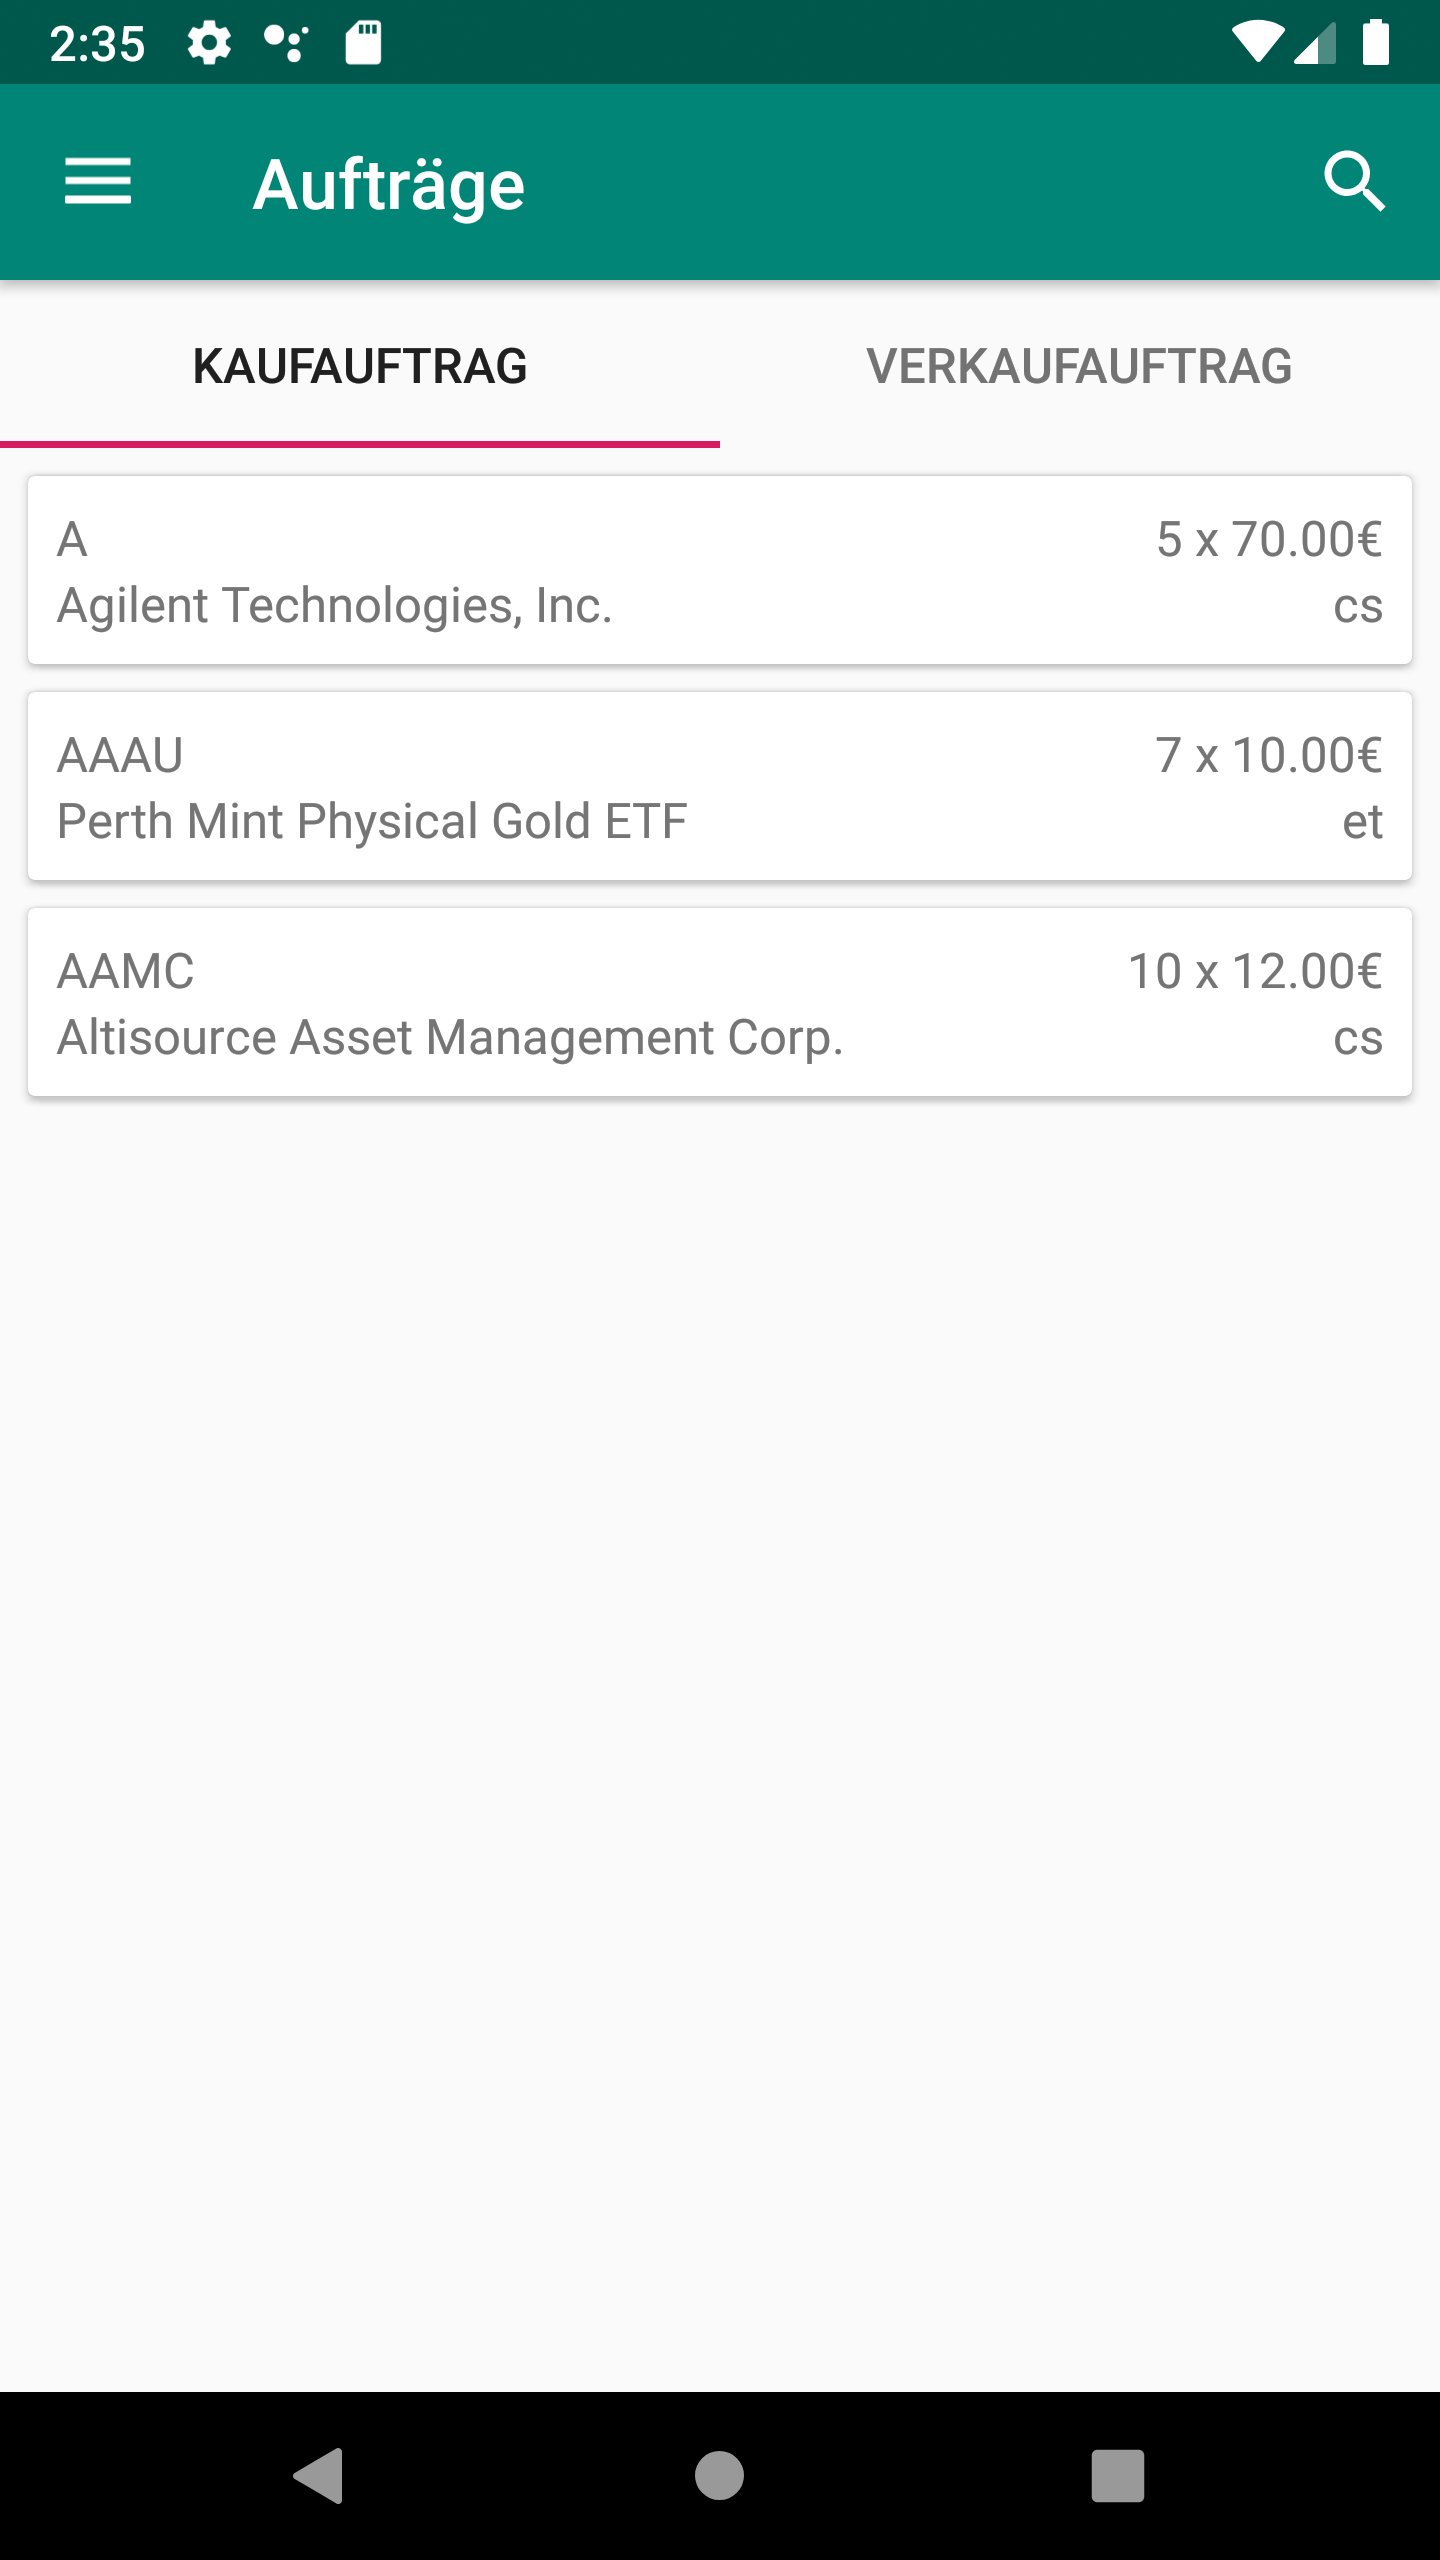
\includegraphics[width=0.6\textwidth]{Bilder/Applikation/Kaufauftrag.png}
	\caption{Kaufaufträge}
\end{figure}

\begin{figure}[H]
	\centering
	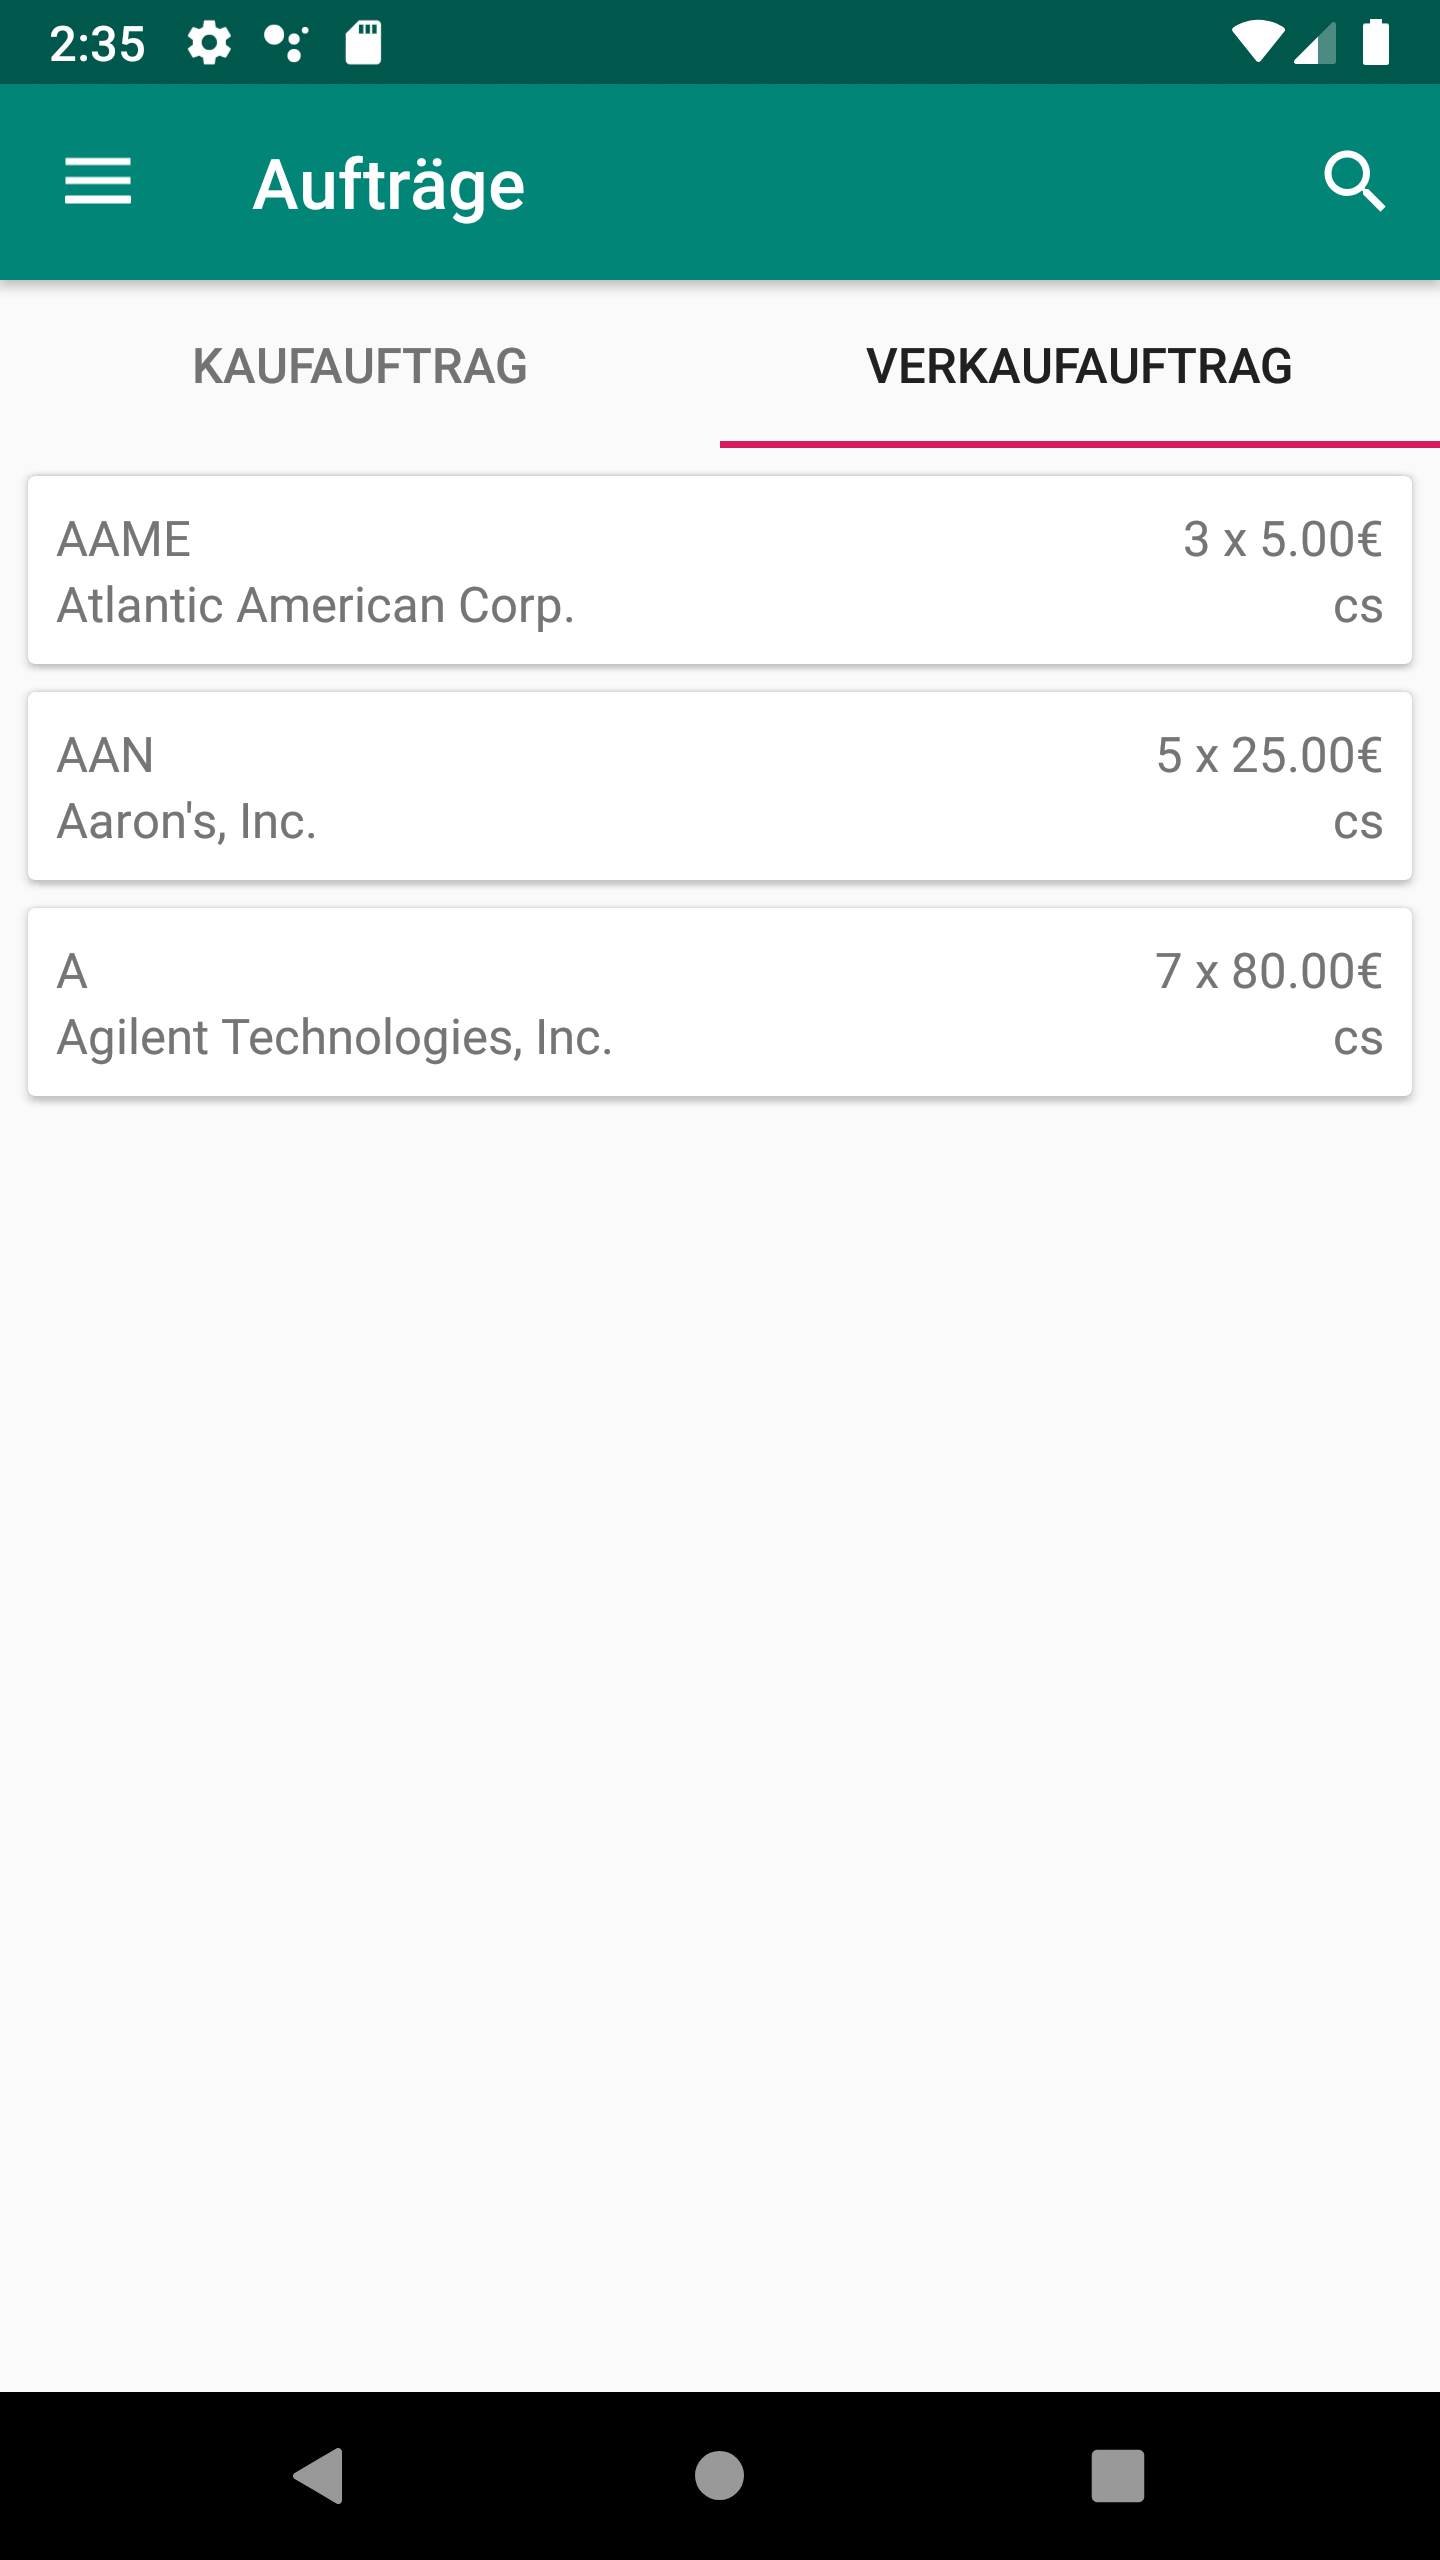
\includegraphics[width=0.6\textwidth]{Bilder/Applikation/Verkaufauftrag.png}
	\caption{Verkaufsaufträge}
\end{figure}

\subsubsection{Suche}
Die Suche ist von Überall erreichbar, nicht nur, wenn man in der Navigation darauf klickt. Auf jeder Seite bindet sich am oberen Ende des Bildschirms eine Leiste, die zur Navigation gehört. Der rechte Teil enthält ein Suchsymbol, dass ein Textfeld in seine Leiste und eine Tastatur öffnet, wenn man darauf klickt. Mit der Tastatur kann man in das Textfeld schreiben und mit Enter seine Suche bestätigen. Durch diesen Prozess gelangt man zu der Hauptseite der Suche und die Aktien, die mit der Eingabe in Verbindung stehen, werden aufgelistet. Jeder Teil der aufgelisteten Aktien führt wieder zu der dazugehörigen Aktiendetailansicht. Über der Liste der Suchergebnisse steht unter anderem "Suchkategorie:". Rechts davon steht am Anfang "Server" und noch weiter rechts davon ein kleines Dreieck mit der Spitze nach unten. Durch drücken auf den Teil zwischen dem Anfang von "Server" und dem Dreieck, fährt ein Menü aus, dass die Kategorien "Kryptowährungen" und "Aktien" beinhaltet, die man durch Klick wählen kann. Die Liste past sich daraufhin auf die Ergebnisse mit der gewählten Kategorie an. Der Text "Server" wird durch den Namen der gewählten Kategorie ersetzt.

"Server" beinhaltet die zehn relevantesten Aktien, "Kryptowährungen" und "Aktien" alle zu ihrer Kategorie gehörenden Ergebnisse.

Gelangt man durch den Eintrag in der Navigation zur Suche, so ist die Seite leer, wenn man vorher nichts gesucht hat. Hat man allerdings schon mal etwas gesucht, so findet man die Seite in dem Zustand, wie sie zuletzt verlassen wurde.

\begin{figure}[H]
	\centering
	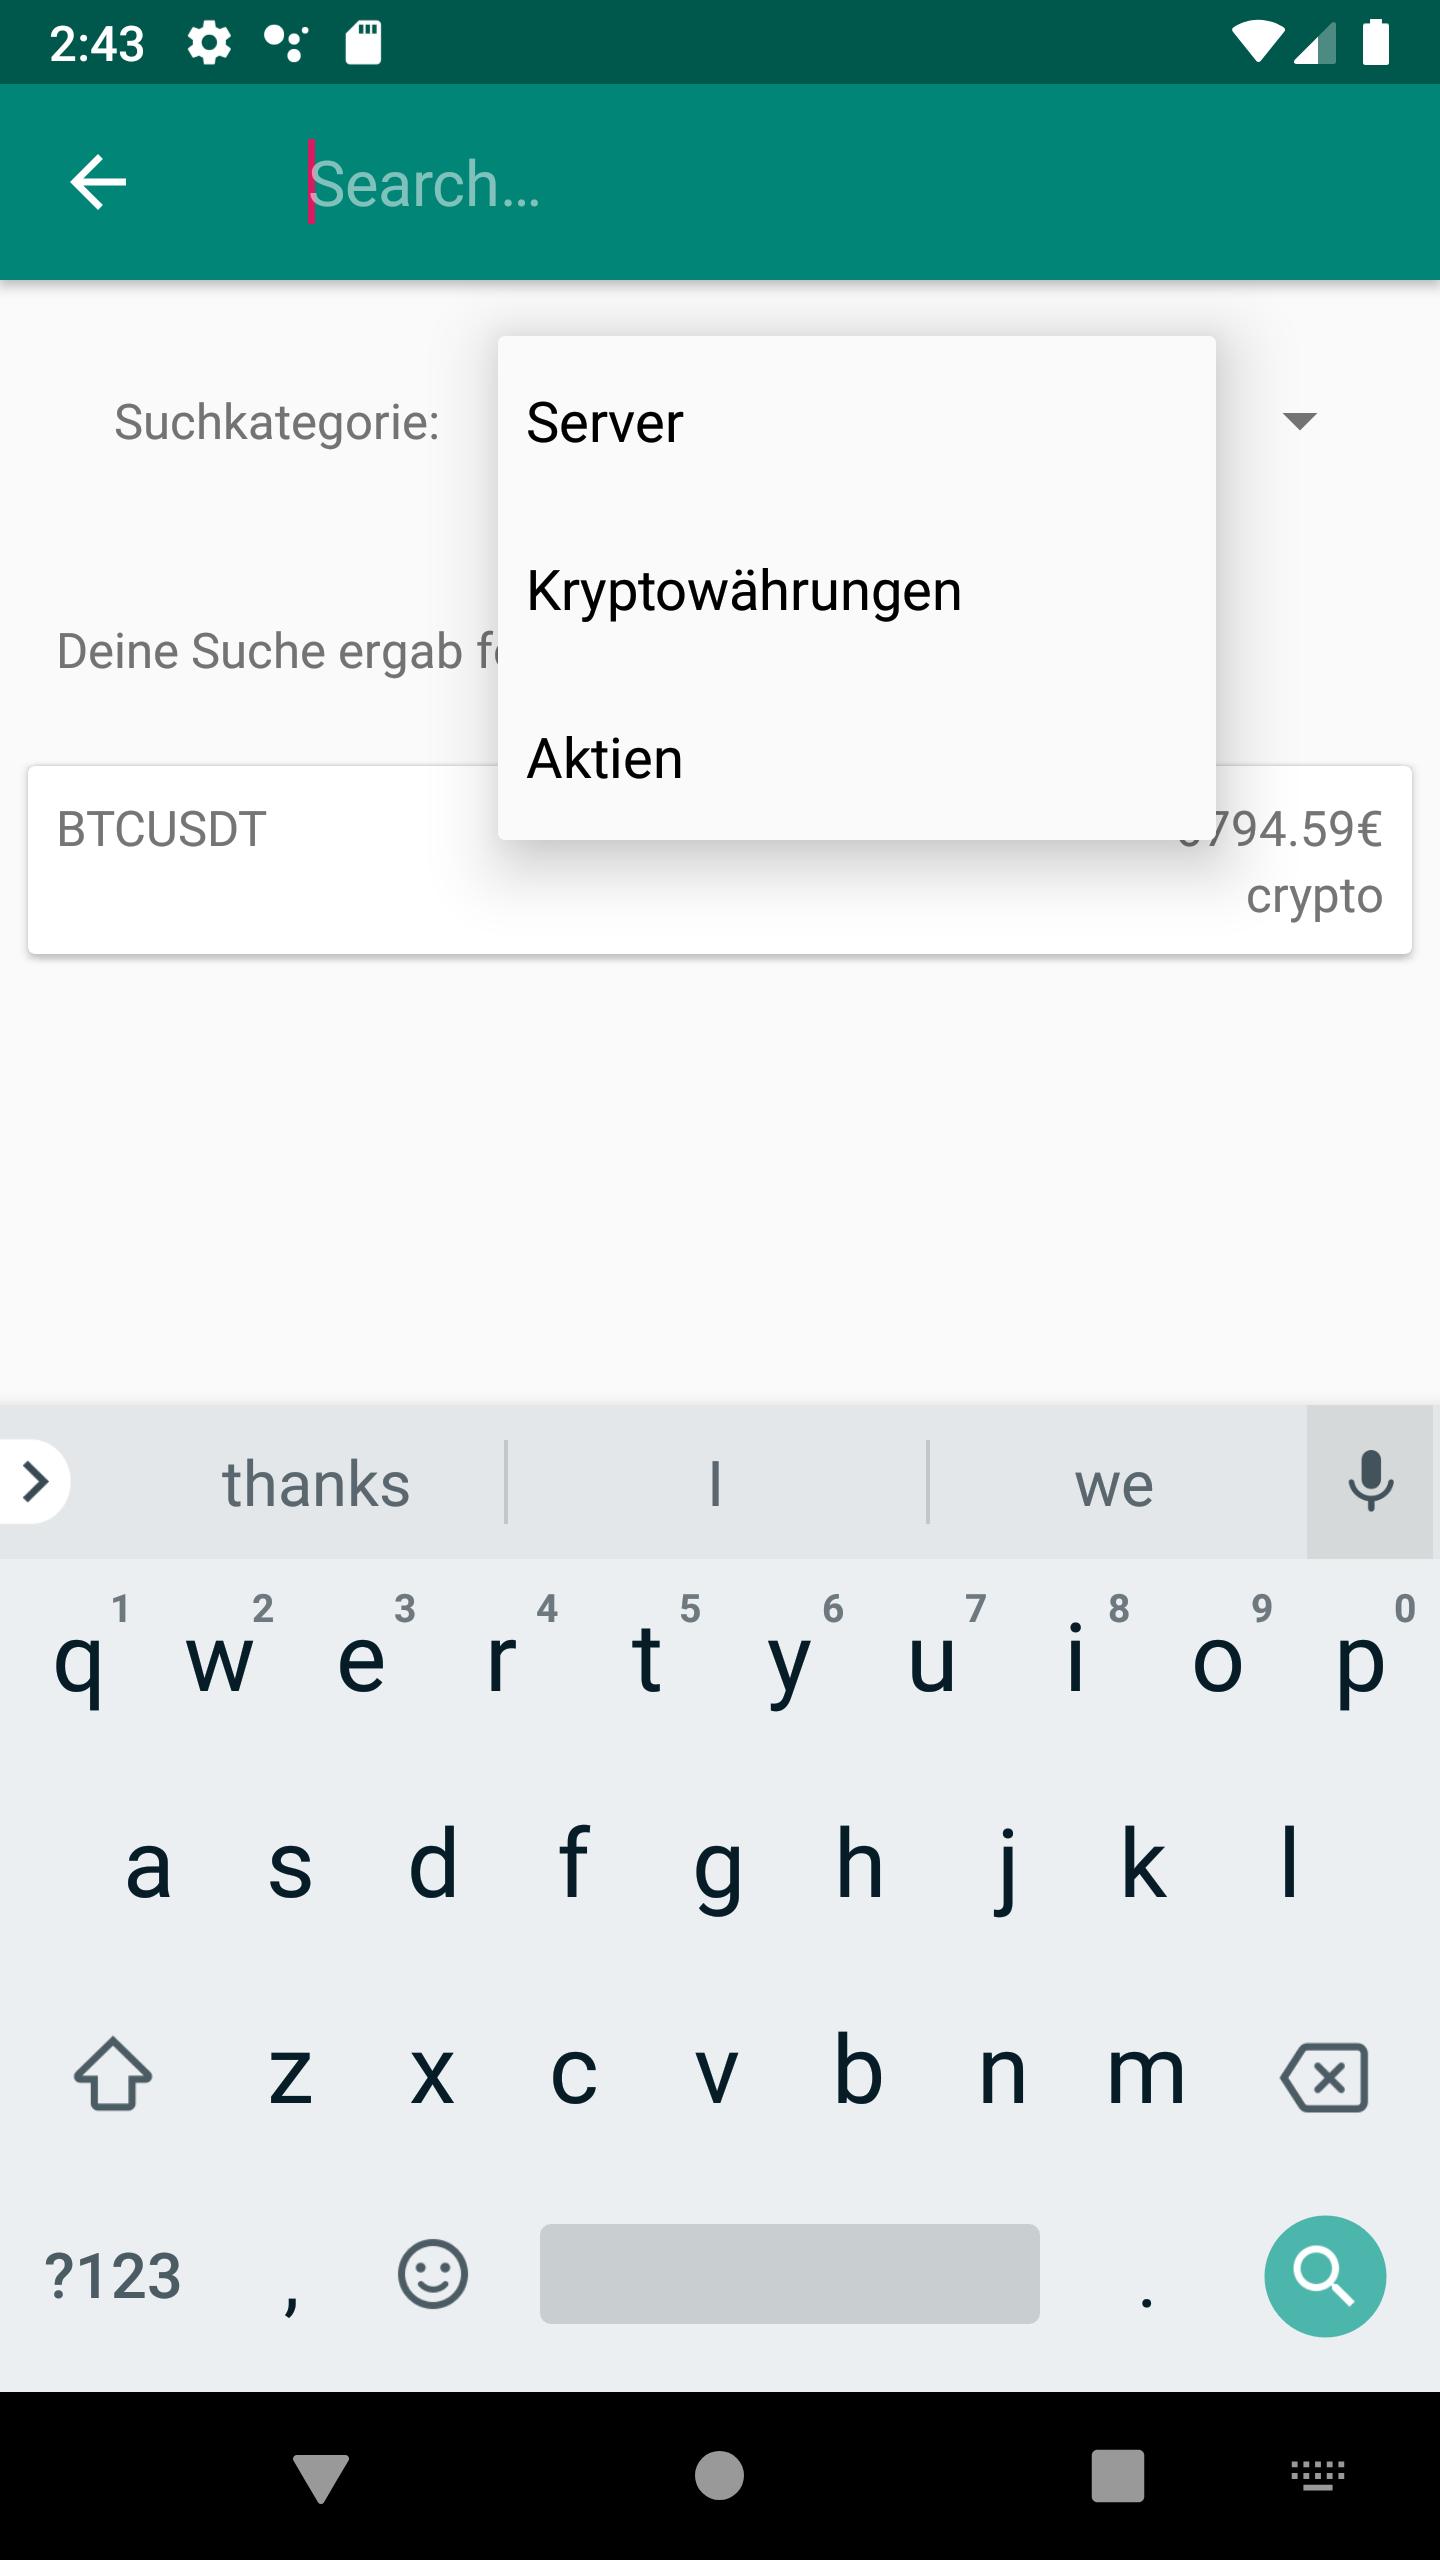
\includegraphics[width=0.6\textwidth]{Bilder/Applikation/Suche.png}
	\caption{Erfolgreiche Suche, oben Suchfeld und Tastatur. Suchkategorien ausgeklappt.}
\end{figure}

\subsubsection{Historie}

Die Historie gibt einen Überblick über alle Käufe und Verkäufe von Aktien, sowie die Bilanz und aktuellen Besitz. Zu beginn des Spiels, bevor man irgendwelche Käufe oder Verkäufe durchgeführt hat, ist die Historie hoch leer und nur am unteren Ende des Bildschirms stehen Werte für Cash, Wertpapieren und die Bilanzsumme. Kauft oder Verkauft man nun jedoch Aktien, tauchen diese Aktionen von oben nach unten in der Reihenfolge der Ausführung auf. Die Einträge bestehen zu Erst aus entweder Plus oder Minus. Plus für Kauf, Minus für Verkauf der Aktien. Dahinter die Anzahl und ein "x" für Mal, und dann den Namen der Aktie. Darauf folgt dann eine freie Stelle, hinter der die Summe des Kauf- oder Verkaufspreises der einzelnen Aktien steht. Ganz rechts vom Eintrag befindet sich noch ein Dollarzeichen, dass zu dem Preis gehört.

Jeder Eintrag beeinflusst die darunterliegenden Werte von Cash, Wertpapieren und Bilanzsumme und diese passen sich entsprechend an.

\begin{figure}[H]
	\centering
	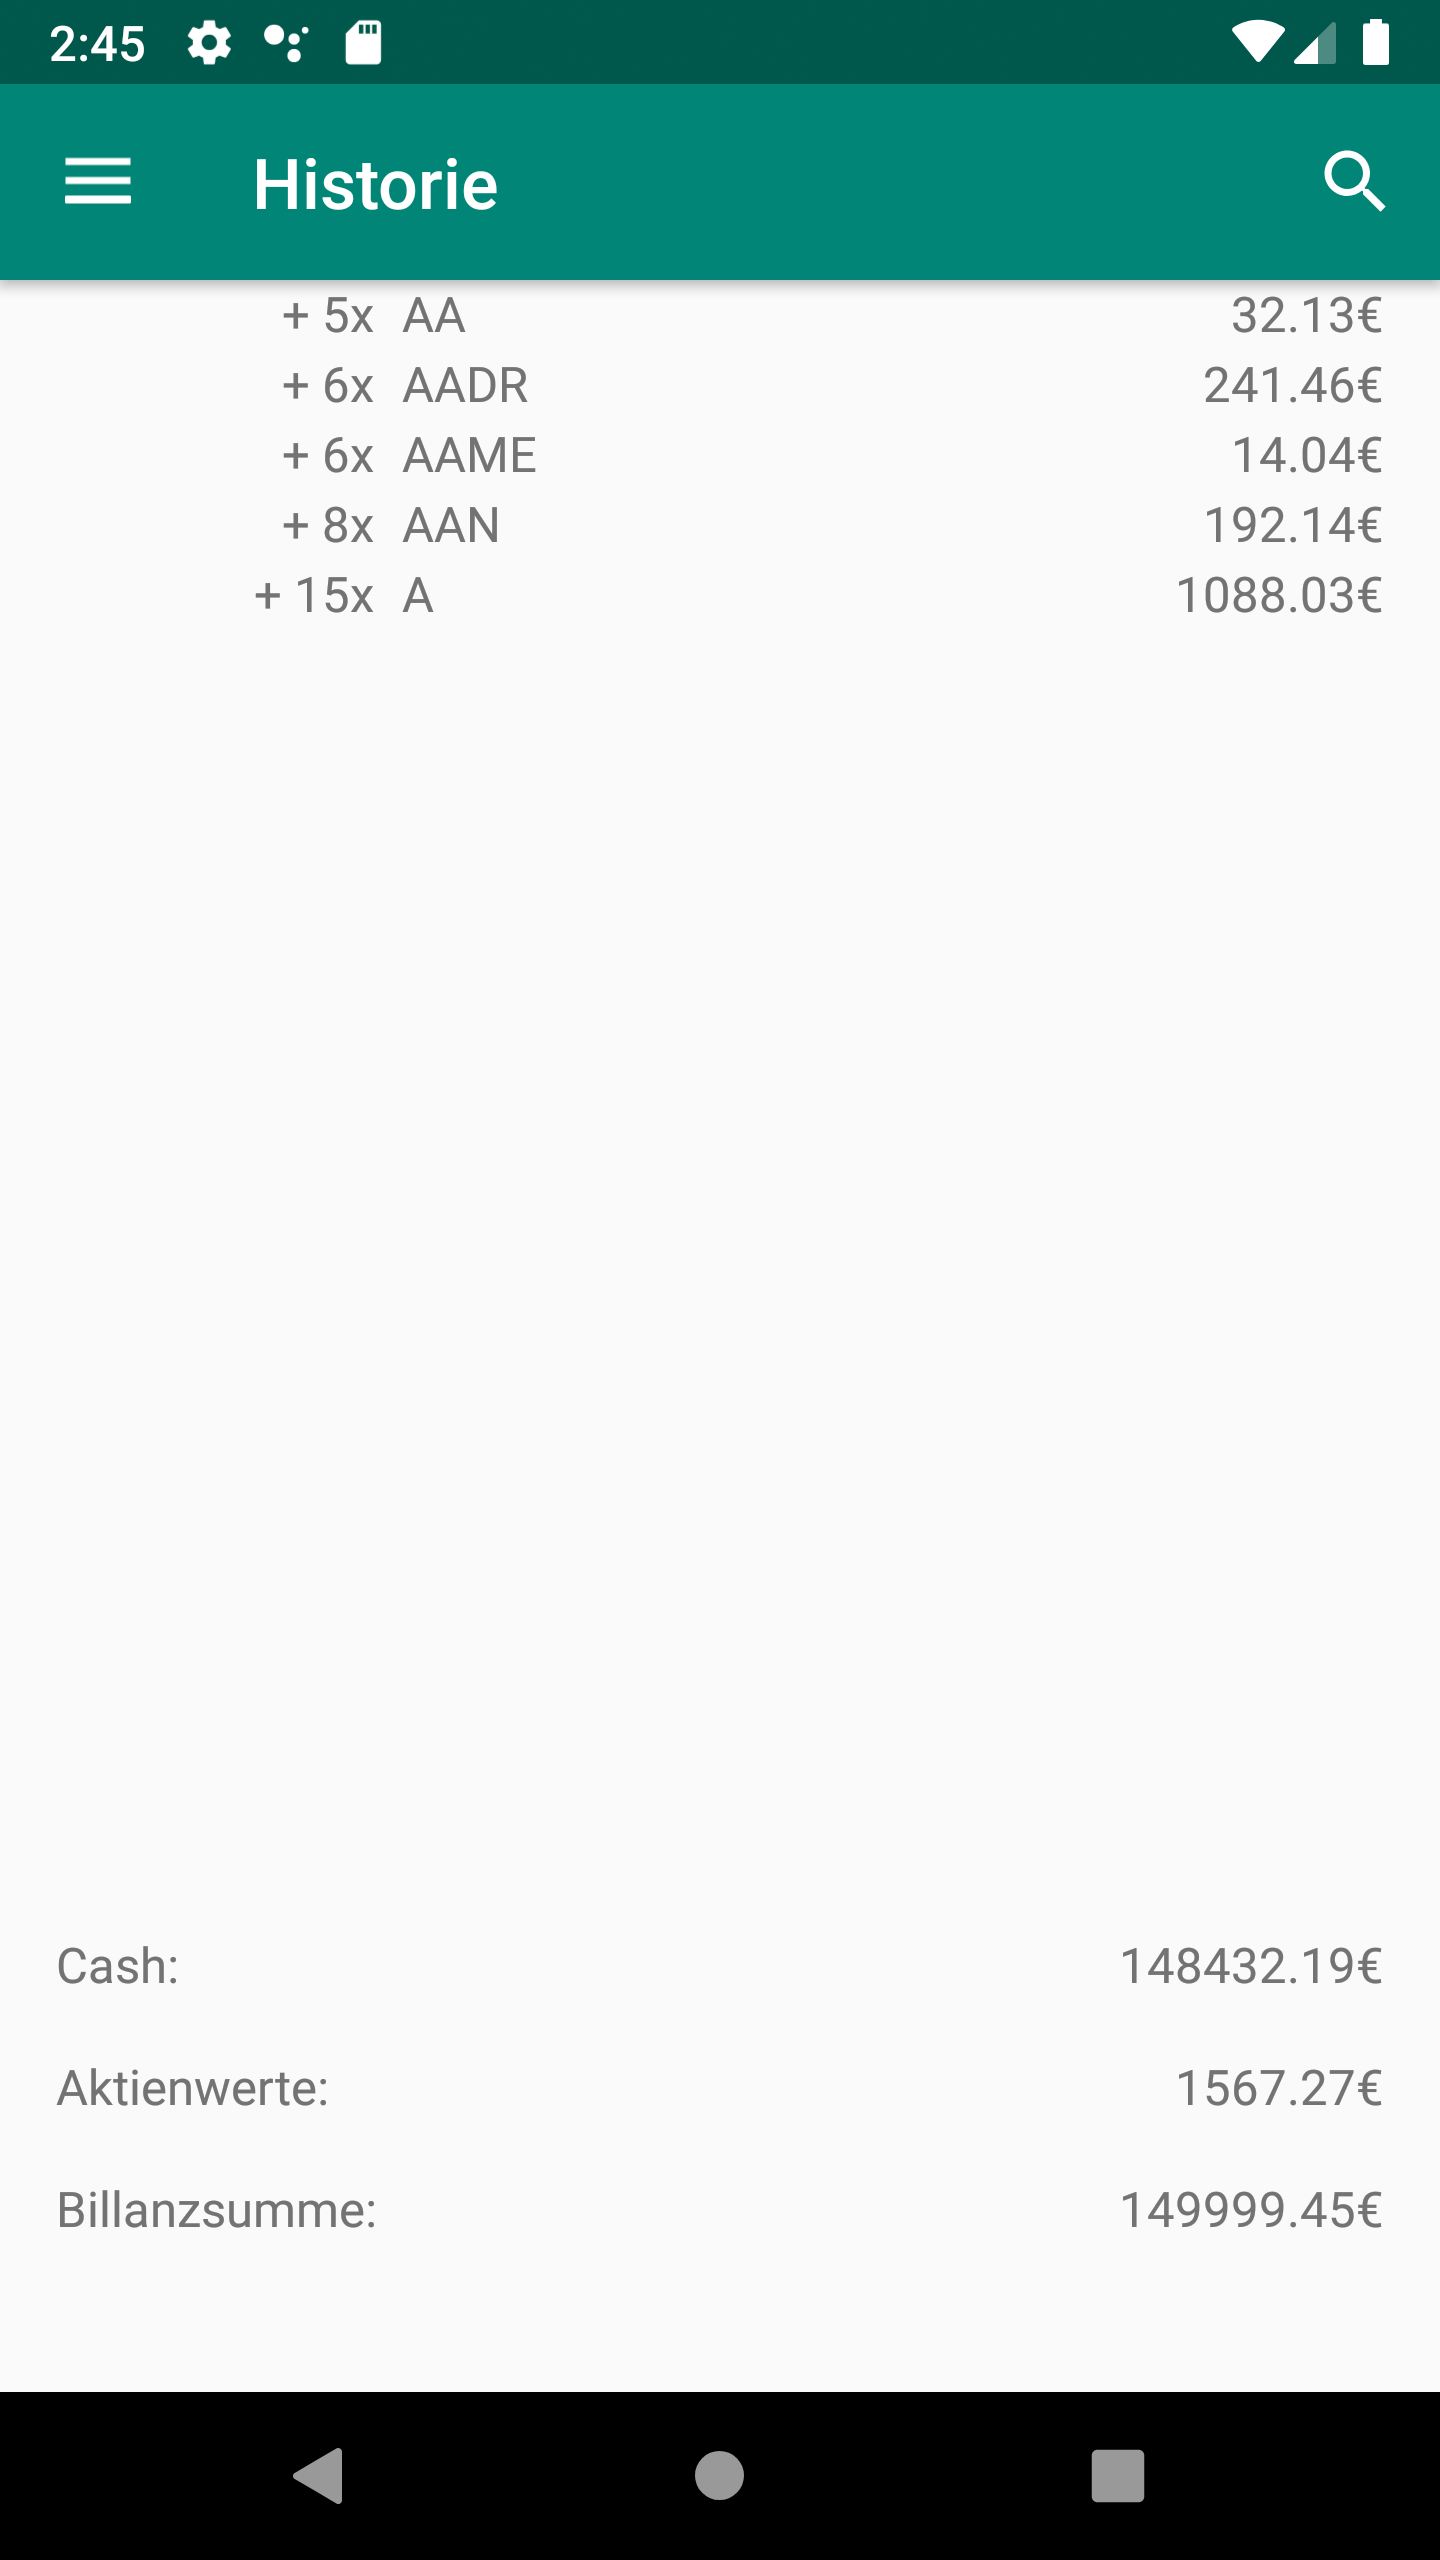
\includegraphics[width=0.6\textwidth]{Bilder/Applikation/Historie.png}
	\caption{Historie}
\end{figure}

\subsubsection{Erfolge}

\begin{figure}[H]
	\centering
	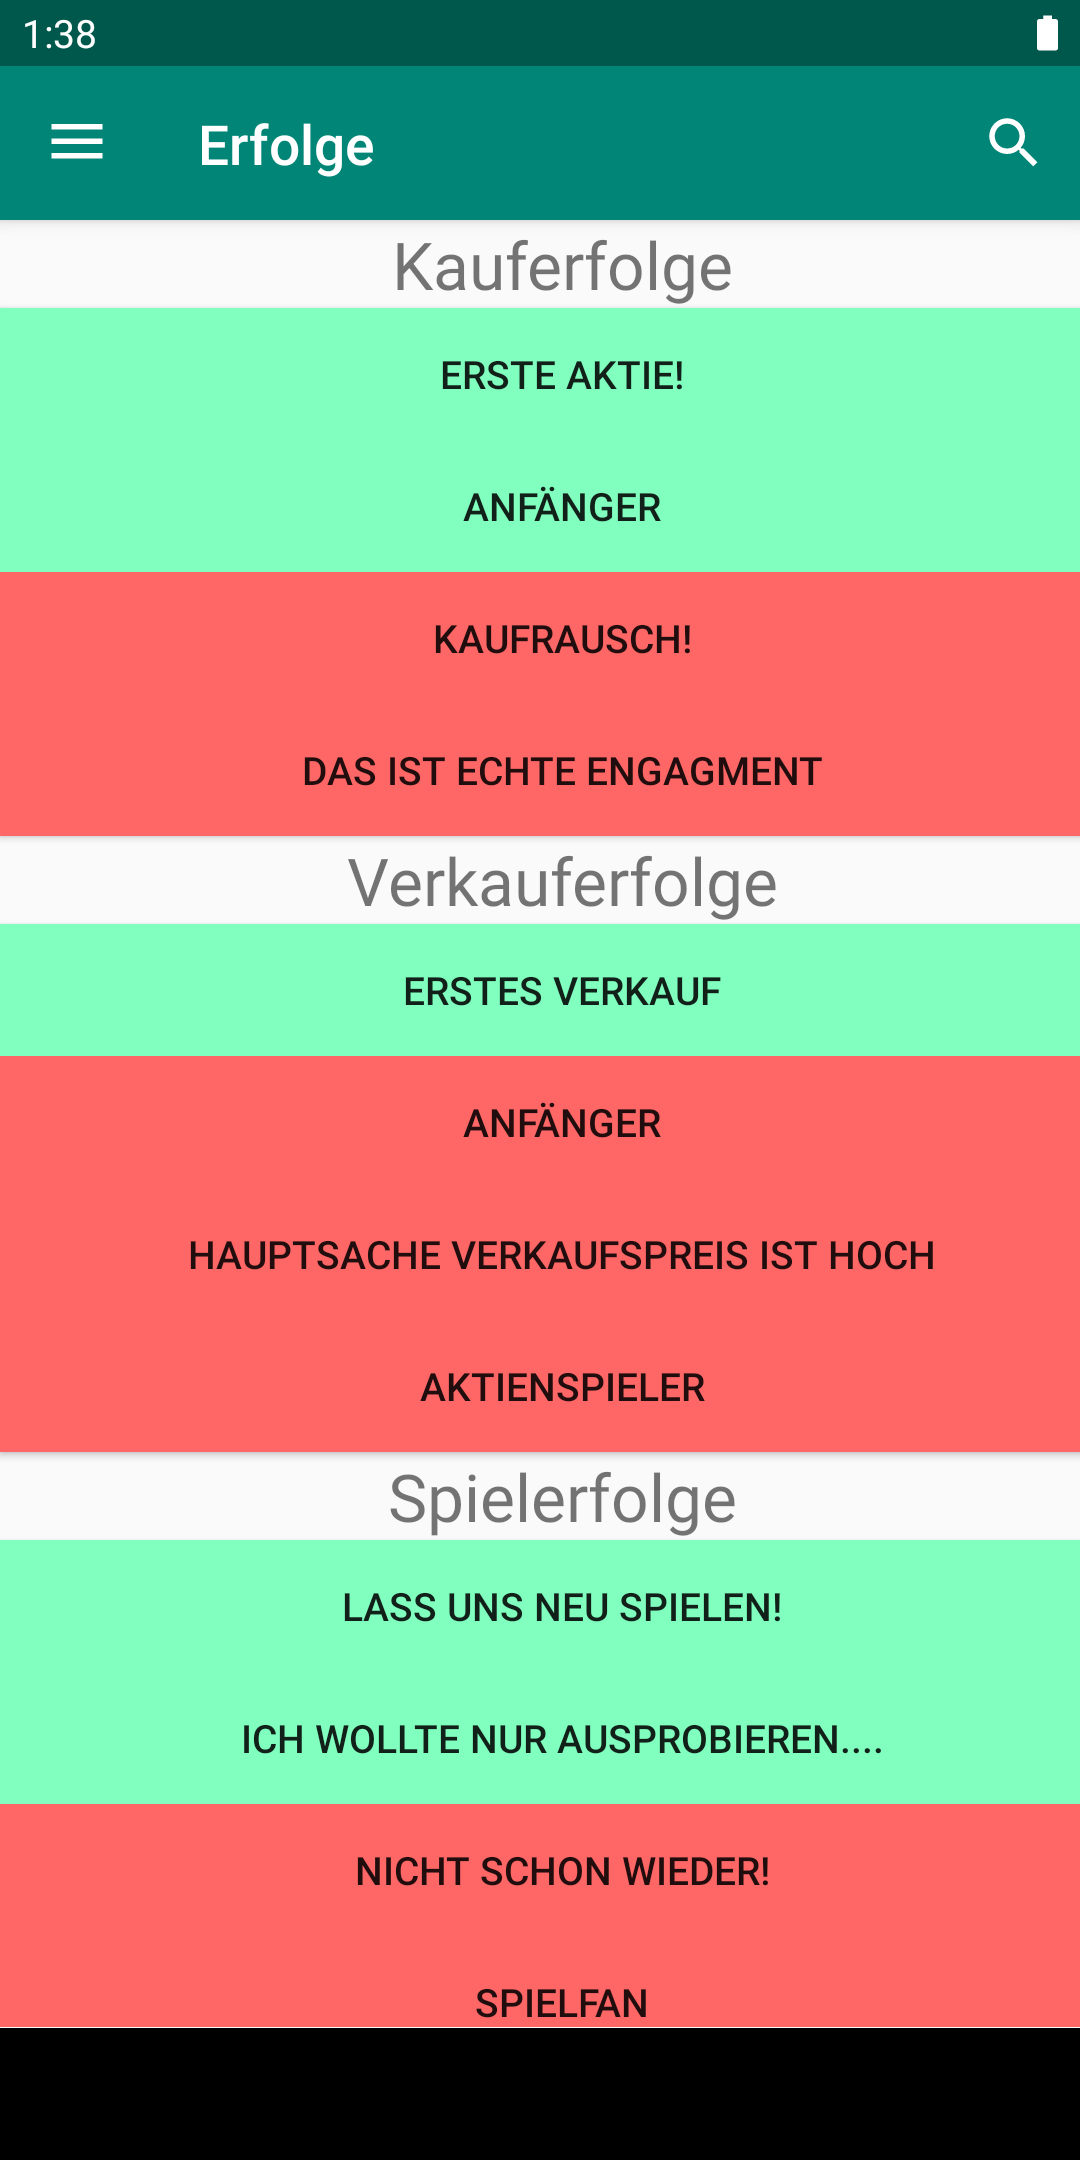
\includegraphics[width=0.6\textwidth]{Bilder/Applikation/erfolge.png}
	 \caption{Erfolge Screen}
	 \label{erfolge1}
\end{figure}

Im Fig.~\ref{erfolge1} kann man das Erfolge Screen sehen. Da sind alle Erfolge aufgelistet, die man im Spiel bekommen kann. Diese sind in 3 Kategorien aufgeteilt:
 \begin{enumerate}
 	\item Kauferfolge
 	\item Verkauferfolge
 	\item Spielerfolge
 \end{enumerate}
Kauf- und Verkauferfolge basieren sich auf der Anzahl von durchgeführten Kauf- und Verkaufsoperationen. Es gibt jeweils 4 Stufen, um die zu bekommen muss man dementsprechend 1, 10, 100 und 1000 Kauf- und Verkaufsoperationen durchführen.

Erste drei Spielerfolge basieren sich auf die Anzahl von Neustarts, dafür muss man entsprechend 1, 5 und 10 das Spiel neu starten. Das Erfolg "Spielfan" bekommt man nur dann, wenn man alle andere Erfolge schon bekommen hat.

Die schon erreichte Erfolge sind grün gefärbt und die, die man noch nicht bekommen hat, sind rot. Jedes Erfolg kann man nur ein Mal bekommen. Diese werden gespeichert und bei der Neustart vom Spiel nicht zurückgesetzt.

\begin{figure}[H]
	\centering
	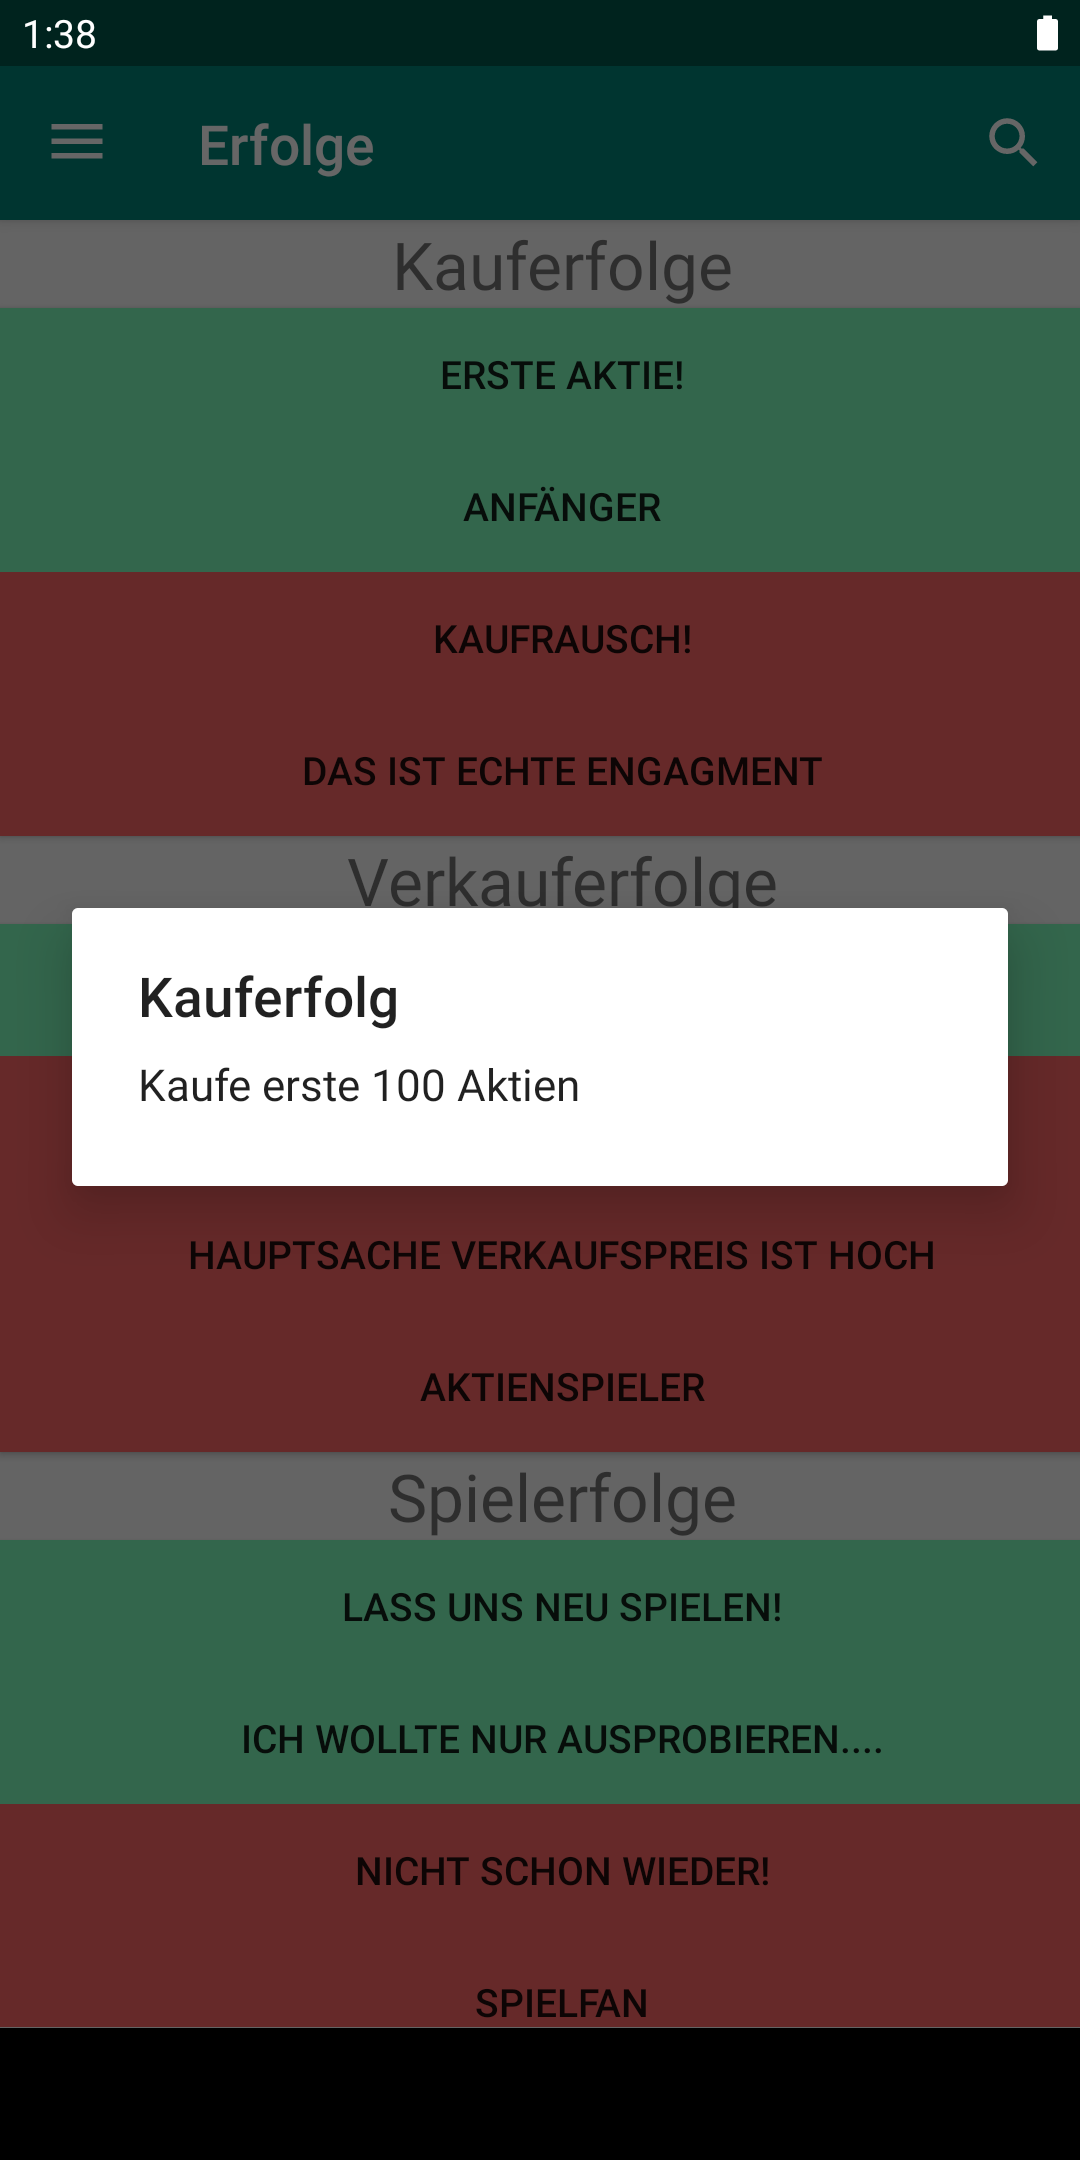
\includegraphics[width=0.6\textwidth]{Bilder/Applikation/erfolgeDetalien.png}
	\caption{Anzeige von Anforderungen um ein Erfolg zu bekommen}
	\label{erfolge2}
\end{figure}

Fig.~\ref{erfolge2} bildet ab, was man sieht, wenn man auf einen bestimmten Erfolg drückt. Dabei kommt ein Dialogfenster, wo die Bedingungen für dieses Erfolg beschrieben sind.

\subsubsection{New Game}

Die letzte Hauptseite "NewGame" gibt die Möglichkeit den Spielstand zurückzusetzen und von vorne zu beginnen. 

Auf der Seite steht nur die Frage, ob man sein Spiel wirklich neu beginnen möchte, der aktuelle Kontostand, den man damit zurücksetzt und ein roter Knopf mit dem Schriftzug "Zurücksetzen" darauf. Drückt man den Knopf, öffnet sich ein Popover, in dem man darauf hingewiesen wird, dass man damit auch alle Aktien im Besitz und die Favoriten löscht. Hier besteht noch die Möglichkeit auf "Abbruch" zu klicken. Drückt man nun jedoch auf "Ok", löschen sich alle spielstandrelevanten Daten. Man landet in einem leeren Depot aber kann direkt mit dem neuen Spielstand weiter spielen.

\begin{figure}[H]
	\centering
	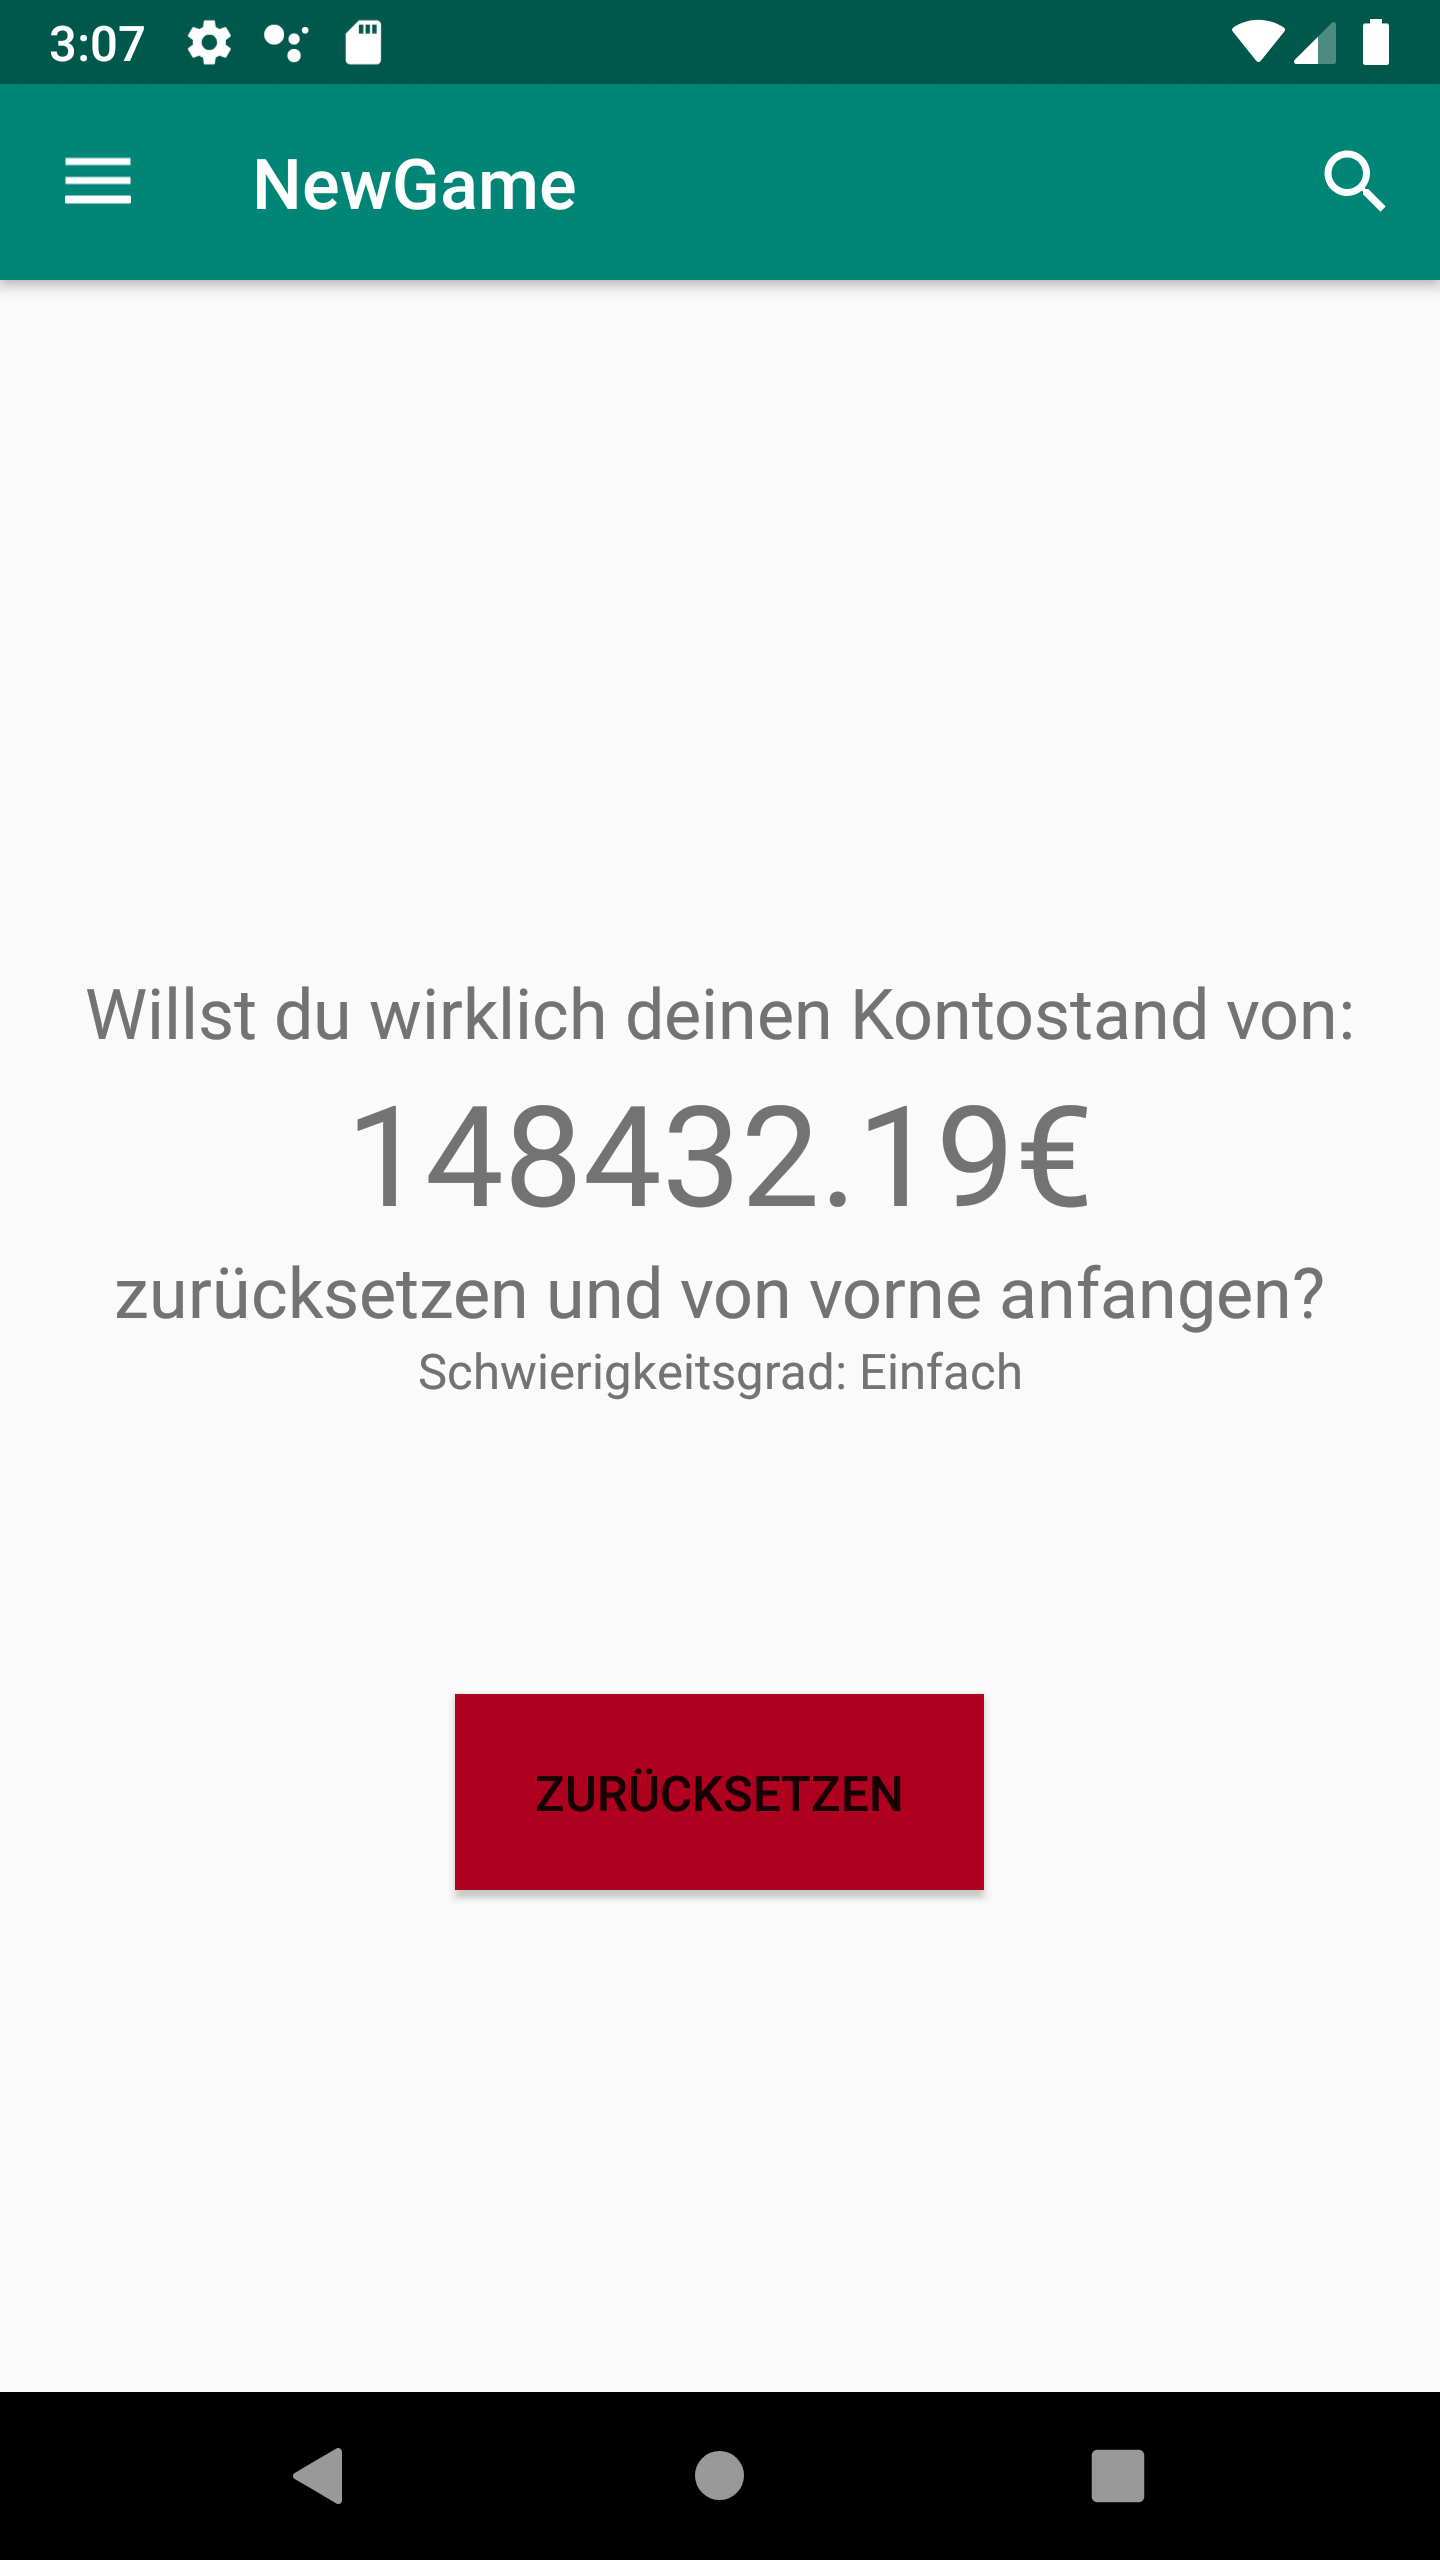
\includegraphics[width=0.6\textwidth]{Bilder/Applikation/NewGame.png}
	\caption{Die Seite NewGame}
\end{figure}

\begin{figure}[H]
	\centering
	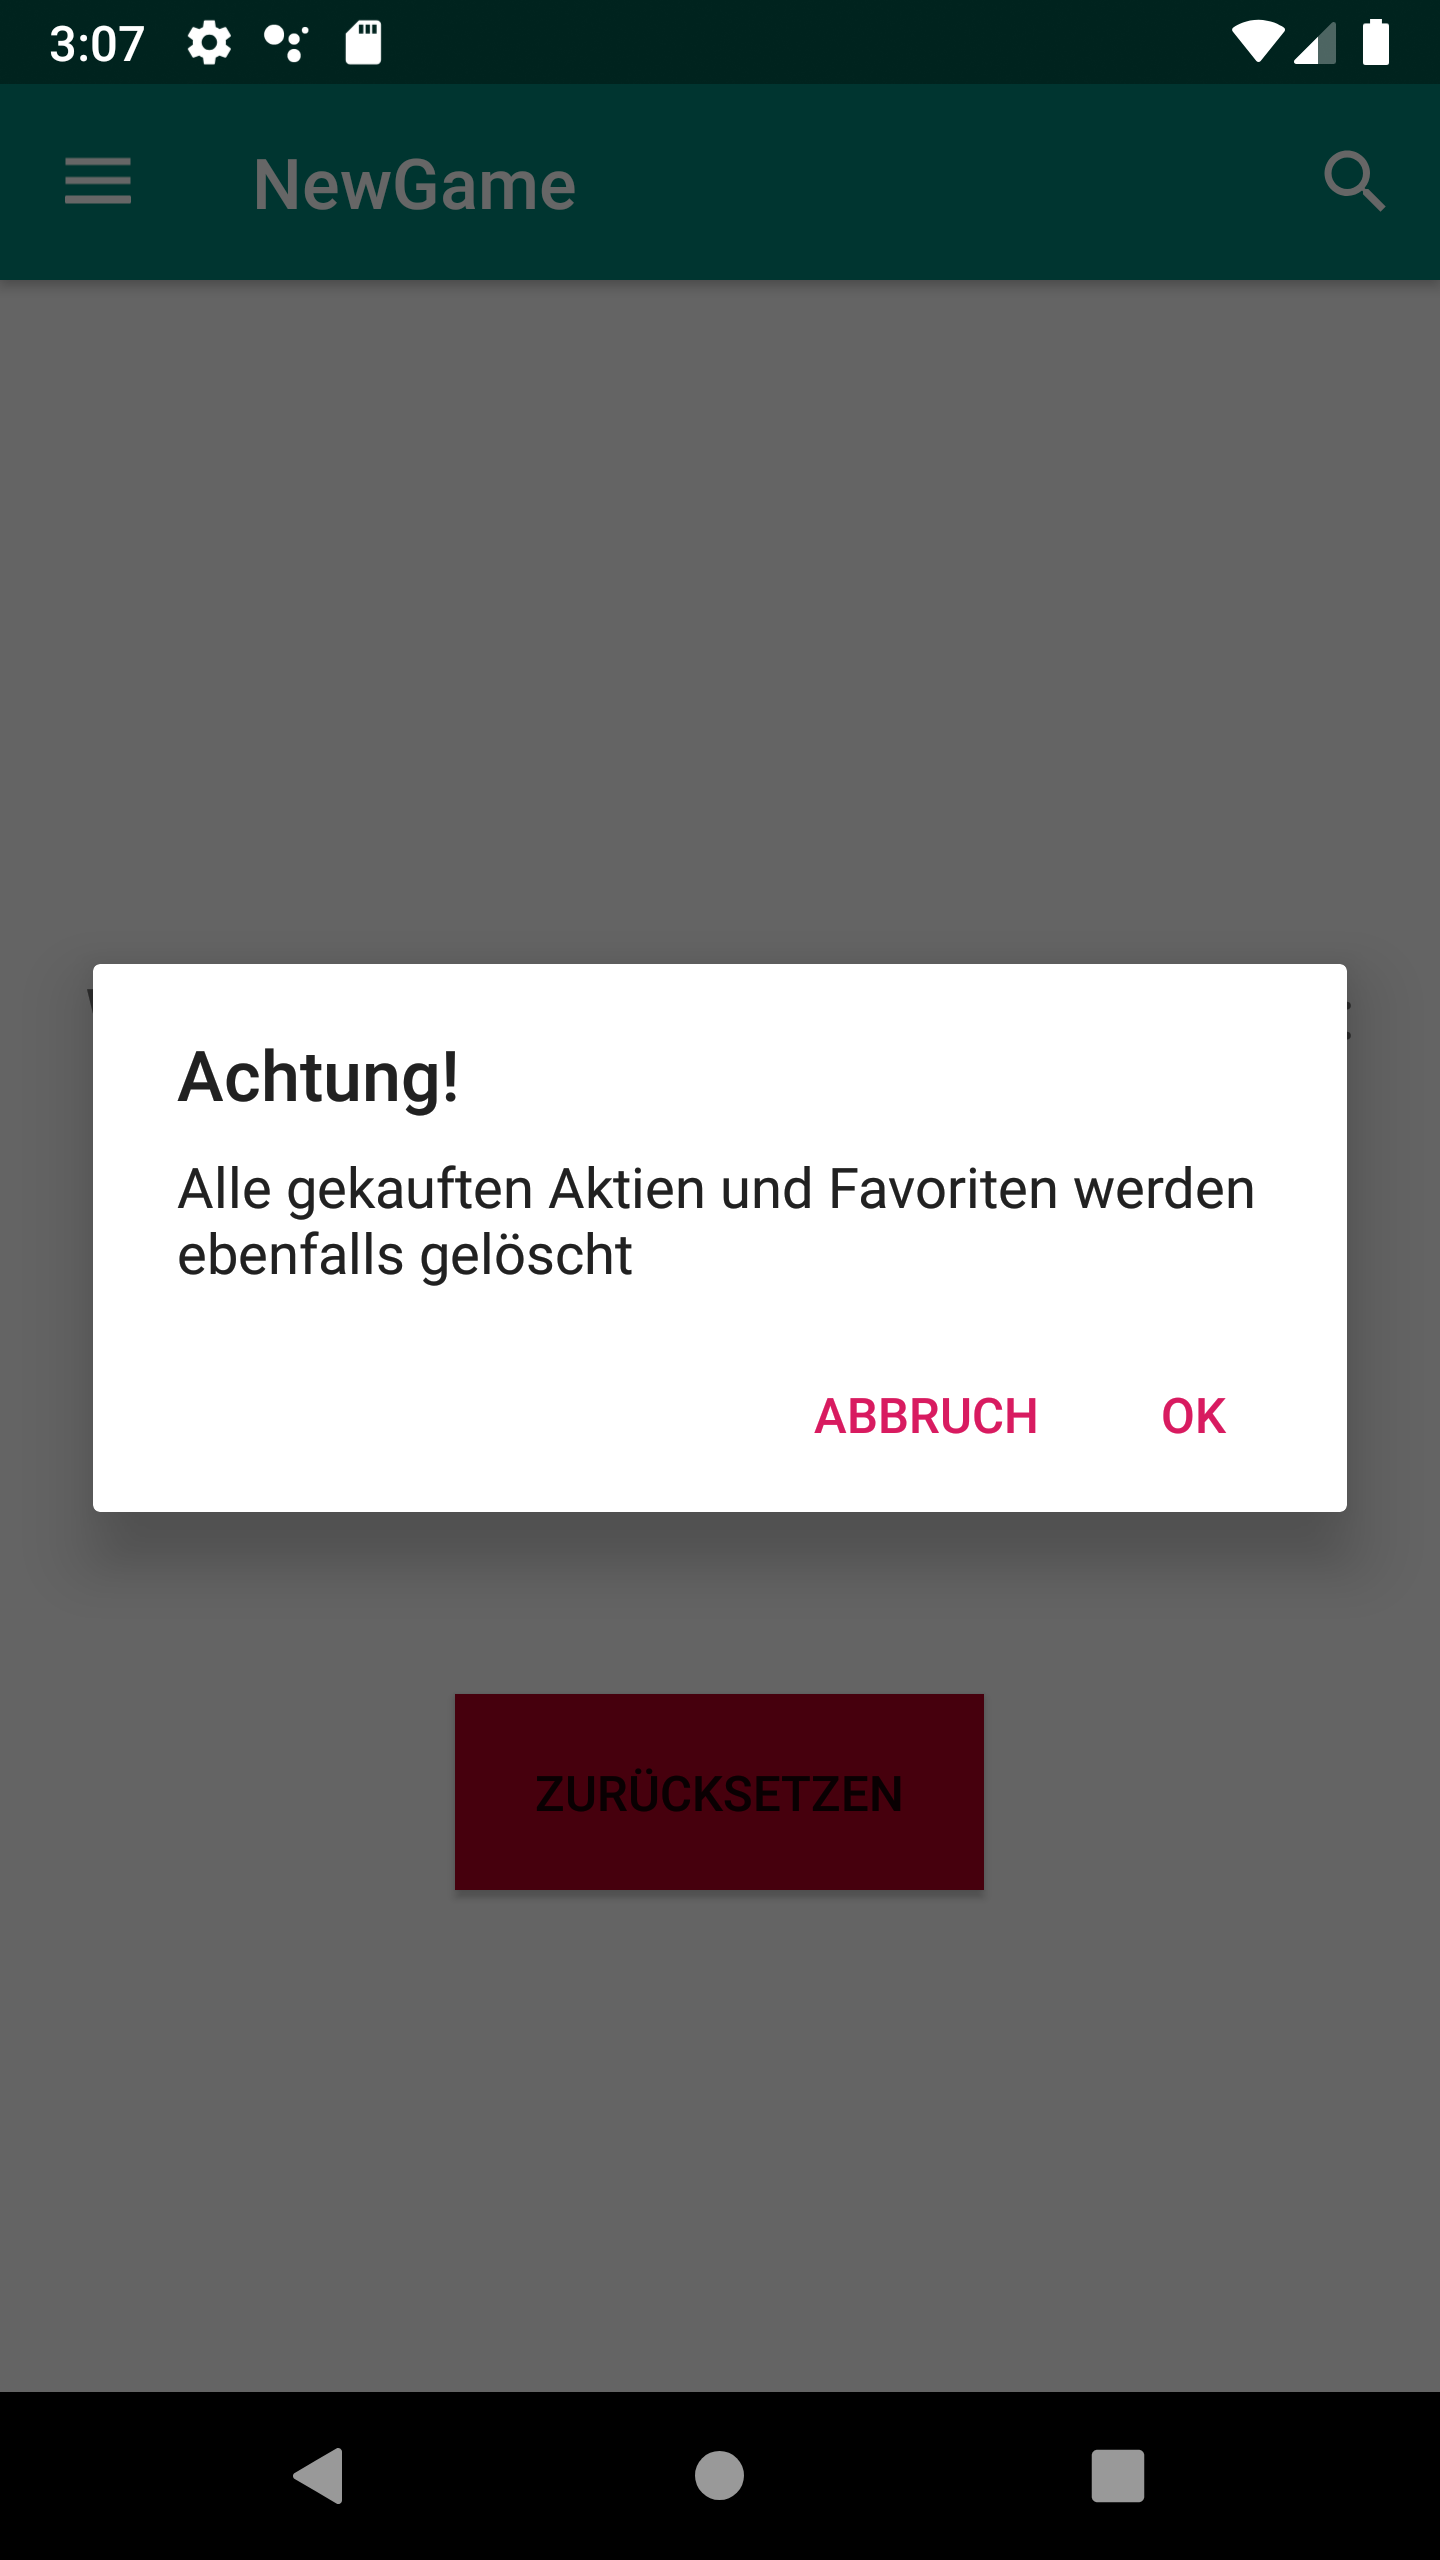
\includegraphics[width=0.6\textwidth]{Bilder/Applikation/NewGameBestaetigung.png}
	\caption{NewGame Bestätigung}
\end{figure}

\todo{schwierigkeitsgrad}
\subsection{Liste aller Klassen und deren Methoden mit Funktion}

\section{Klassendiagramm}

\subsection{Anbindung an das Datenmodell der API}

\subsection{Darstellung des Datenmodells als UML}

\subsection{Darstellung aller Views und deren Controller als UML}

\section{Vorstellung der Application}
%Hier ist wichtig zu schreiben, was wir meinen Gut gemacht ist und wie dies mit den App zielen conquentiert.

\subsection{Vorstellung der Grundfunktionen}
In diesem Abschnitt werden die geforderten Grundfunktionen dargestellt. In des Rahmen Seminars wurden folgende Anforderungen gestellt:
\newline
Folgende Grundfunktionen wurden implementiert:
\begin{enumerate}
	\item Die Suche nach Aktien, Währungen, Digitalwährungen
	\item Portfolio anlegen
	\item Depotübersicht
	\item Kontostand + Verlauf
	\item Transaktionskosten
	\item Aktien kaufen/verkaufen(Live Trading)
	\item Historie über Käufe und Verkäufe
	\item Automatischer Handel im Hintergrund
	\item Spiel zurücksetzen / neustarten
\end{enumerate}

Folgende Zusatzfunktionen wurden implementiert:

\begin{enumerate}
	\item Aktienhebel
	\item Erfolge
	\item Detailansicht der Aktien
	\item Schwierigkeitsgrad Einstellungen
	\item Persistenz
\end{enumerate}

Dies ist die Java Code Camp präsentation von \todo{Bitte pflegt hier eure Namen!!!} Christian Küllmer, Anna Tsarenko und [].

Die Anforderungen des Java Code Camps wurden von uns im Android Studio Projekt Shares App umgesetzt. Die entstandene App heißt Broken Broke Broker und ist auf auf dem Smartphone unter BBB zu finden.

\begin{figure}[H]
	\centering
	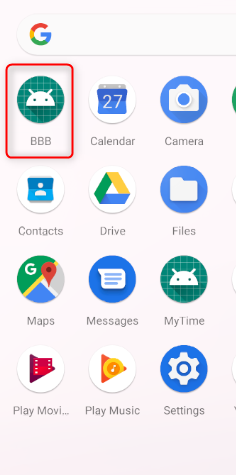
\includegraphics[width=0.6\textwidth]{Bilder/Prsi/StartenDerApp.png}
	\caption{Zum Öffnen der App folgen Sie bitte dieser Instruktion im Menü}
\end{figure}

Im Folgenden soll nun präsentiert werden, welche dieser Funktionen umgesetzt wurden und wie die Anzeichen dieser App innerhalb des funktionieren. Als Kunde soll man hierbei einen Eindruck davon bekommen, welche Vorteile das Produkt für den Kunden hat. 

\subsubsection{Depotübersicht}
Beim Starten der App beginnt man auf der Depotübersicht. Diese Persistent gehaltene Ansicht zeigt die in der App befindlichen gekauften Aktien und es kann direkt abgelesen werden, welchen Wert das eigene Depot zu diesem Zeitpunkt hat. Das schafft eine Übersichtlichkeit des Einstiegsmoments und bringt den Spieler dicht an an das Spielgeschehen.

\begin{figure}[H]
	\centering
	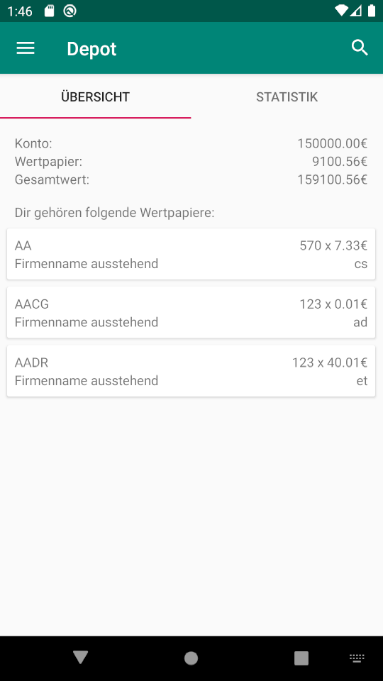
\includegraphics[width=0.6\textwidth]{Bilder/Prsi/einstieg.png}
	\caption{Das Einstiegsbild nach dem Wählen des Schwierigkeitsgrades mit gekauften Aktien}
\end{figure}

Das Einstiegsbild verfolgt weiter was Konzept von einzelnen klaren Farben und einem Sichtbaren Design für die aktuelle Marktlage. Dies ermöglicht volle Kontrolle über die gerade zu besessenen Aktien.
								
\subsubsection{Die Suche nach Aktien, Währungen, Digitalwährungen}

Bei der Suche nach Aktien kann entweder das Symbol einer Aktie oder der Name einer Aktie eingegeben werden um weitere Attribute einer Aktie zur Anzeige zu bringen. Dem Spieler soll damit die Möglichkeit gegeben werden, sich gut über eine Aktie zu informieren. Weiter zeigt der Reiter alle Aktien die den Suchbegriff in Namen oder Symbol tragen. Die Oberfläche der Suche kann dabei in der App auf der Linken Seite gefunden werden und öffnet direkt das Suchmenü.

\begin{figure}[H]
	\centering
	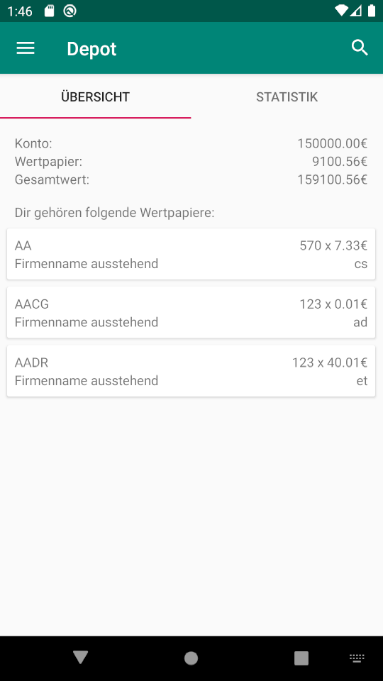
\includegraphics[width=0.6\textwidth]{Bilder/Prsi/einstieg.png}
	\caption{Anzeige der Aktiensuche mit gefüllten Daten}
\end{figure}

Die Anzeige entspricht ebenfalls dem Konzept von einzelnen klaren Farben und einem Sichtbaren Design für die aktuelle Marktlage. Dies ermöglicht volle Kontrolle über suchenden Aktien und keinerlei Ablenkung von den wesentlichen Faktoren.

\subsubsection{Portfolio anlegen}

Das Portfolio wurde als Funktion implementiert um interessante Aktien bei unklarer Marktlage weiter überwachen zu können. Innerhalb der Detailansicht einer Aktie kann eine Aktie zum Portfolio hinzu gefügt werden. Weiter kann jede dem Portfolio hinzugefügte Aktie gelöscht werden. Die Inhalte des Portfolio sind persistent und werden bei jedem laden beibehalten. Eine Prüfung der Aktien im Portfolio findet nicht statt, das bedeutet sollte eine Aktie vom Markt verschwinden kann man sie weiterhin im Portfolio halten.

\begin{figure}[H]
	\centering
	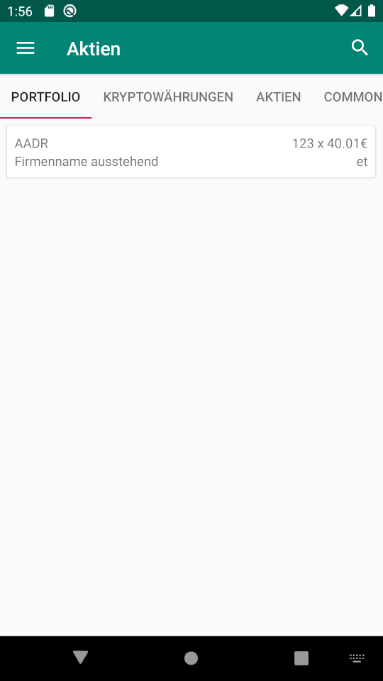
\includegraphics[width=0.6\textwidth]{Bilder/Prsi/Portfolio.png}
	\caption{Anzeige der Aktiensuche mit gefüllten Daten}
\end{figure}

Das Portfolio ist dabei der erste Reiter in dem Tab Aktien und bildet hier die Anforderung Portfolio anlegen komplett ab.

\subsubsection{Depotübersicht}

Innerhalb der Depotübersicht wird die Komplettzahl der gekauften Aktien angezeigt. Dabei wird mit berechnet welchen Wert das aktuelle Depot hat und welcher Geldwert aktuell Materielle und Liquide Güter haben. Dieser Wert wird aktuell gehalten und bildet den Grundstock der daten für die persönliche Statistik.


\begin{figure}[H]
	\centering
	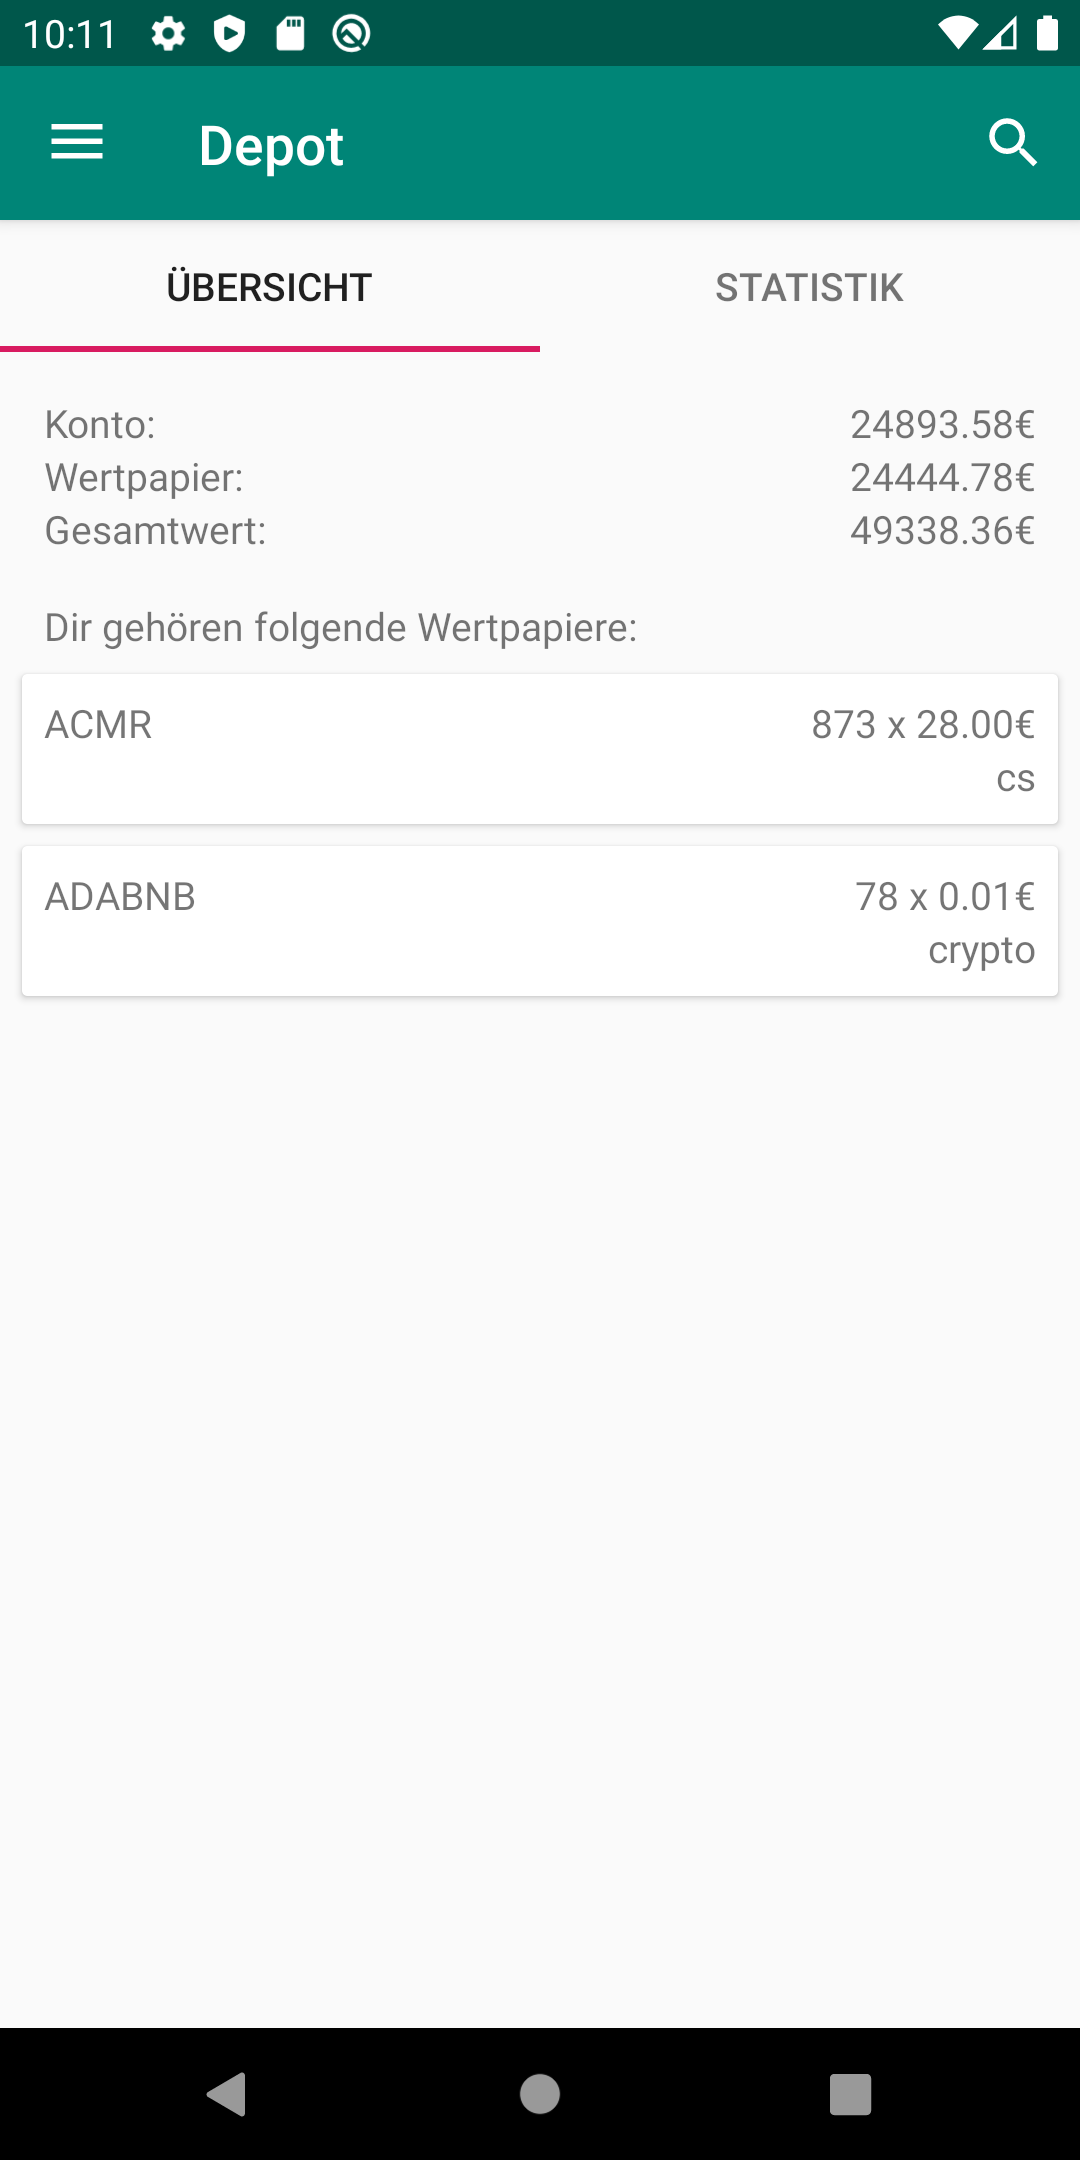
\includegraphics[width=0.6\textwidth]{Bilder/Prsi/depot.png}
	\caption{Anzeige der Aktiensuche mit gefüllten Daten}
\end{figure}
 
Die Übersicht ist so strukturiert, dass die eigenen Aktien einfach im Überblick gehalten werden können. Weiter ist das Anzeigen der Aktien mit einer einfachten Kastenlogik klassisch nach dem Material Design.

\subsubsection{Kontostand + Verlauf}

Den Kontostand und den Verlauf des eigenen Geldes gibt es in der Application Broken Broke Broker in zwei verschiedenen Ansichten. Das Feature Kontostand ist bei uns in der Ansicht des Depos und der Historie zu sehen. Das hat den Grund, dass ein Spieler direkt bei seinen Handlungen und bei seinen Erfolgen sehen soll, wie sein Kontostand aktuell ist. Die eigenen Verläufe sind unter dem Menüeintrag Statistik im Reiter Depot zu finden. Hier wird der Verlauf der bisherigen Transaktionen angezeigt und die entsprechenden Vermögenszuwächse und Verluste. 

Im Folgenden sind die beiden Features Bildlich dargestellt.

\begin{figure}[H]
	\centering
	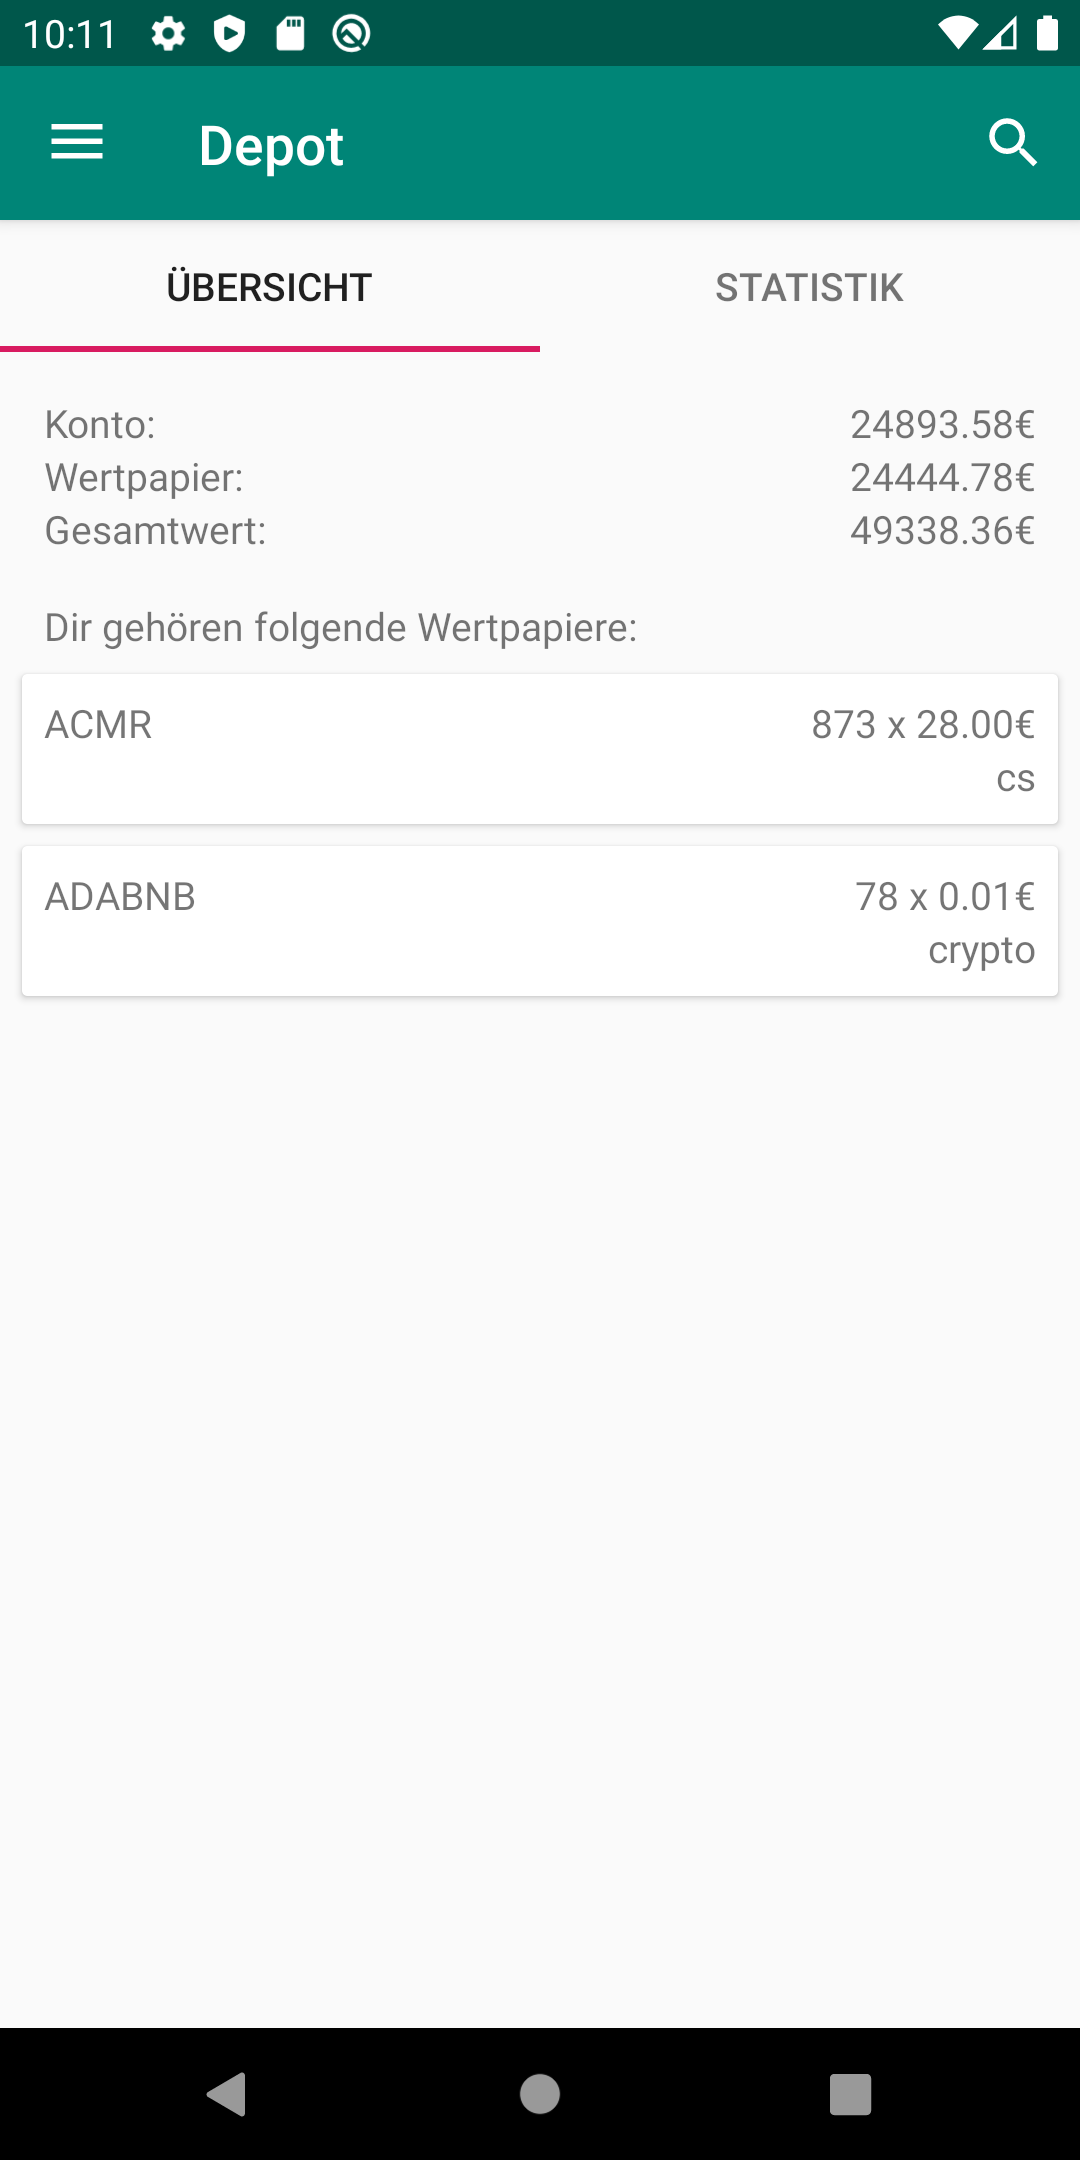
\includegraphics[width=0.6\textwidth]{Bilder/Prsi/depot.png}
	\caption{Wahrenverkehrswert des Depots}
\end{figure}

\begin{figure}[H]
	\centering
	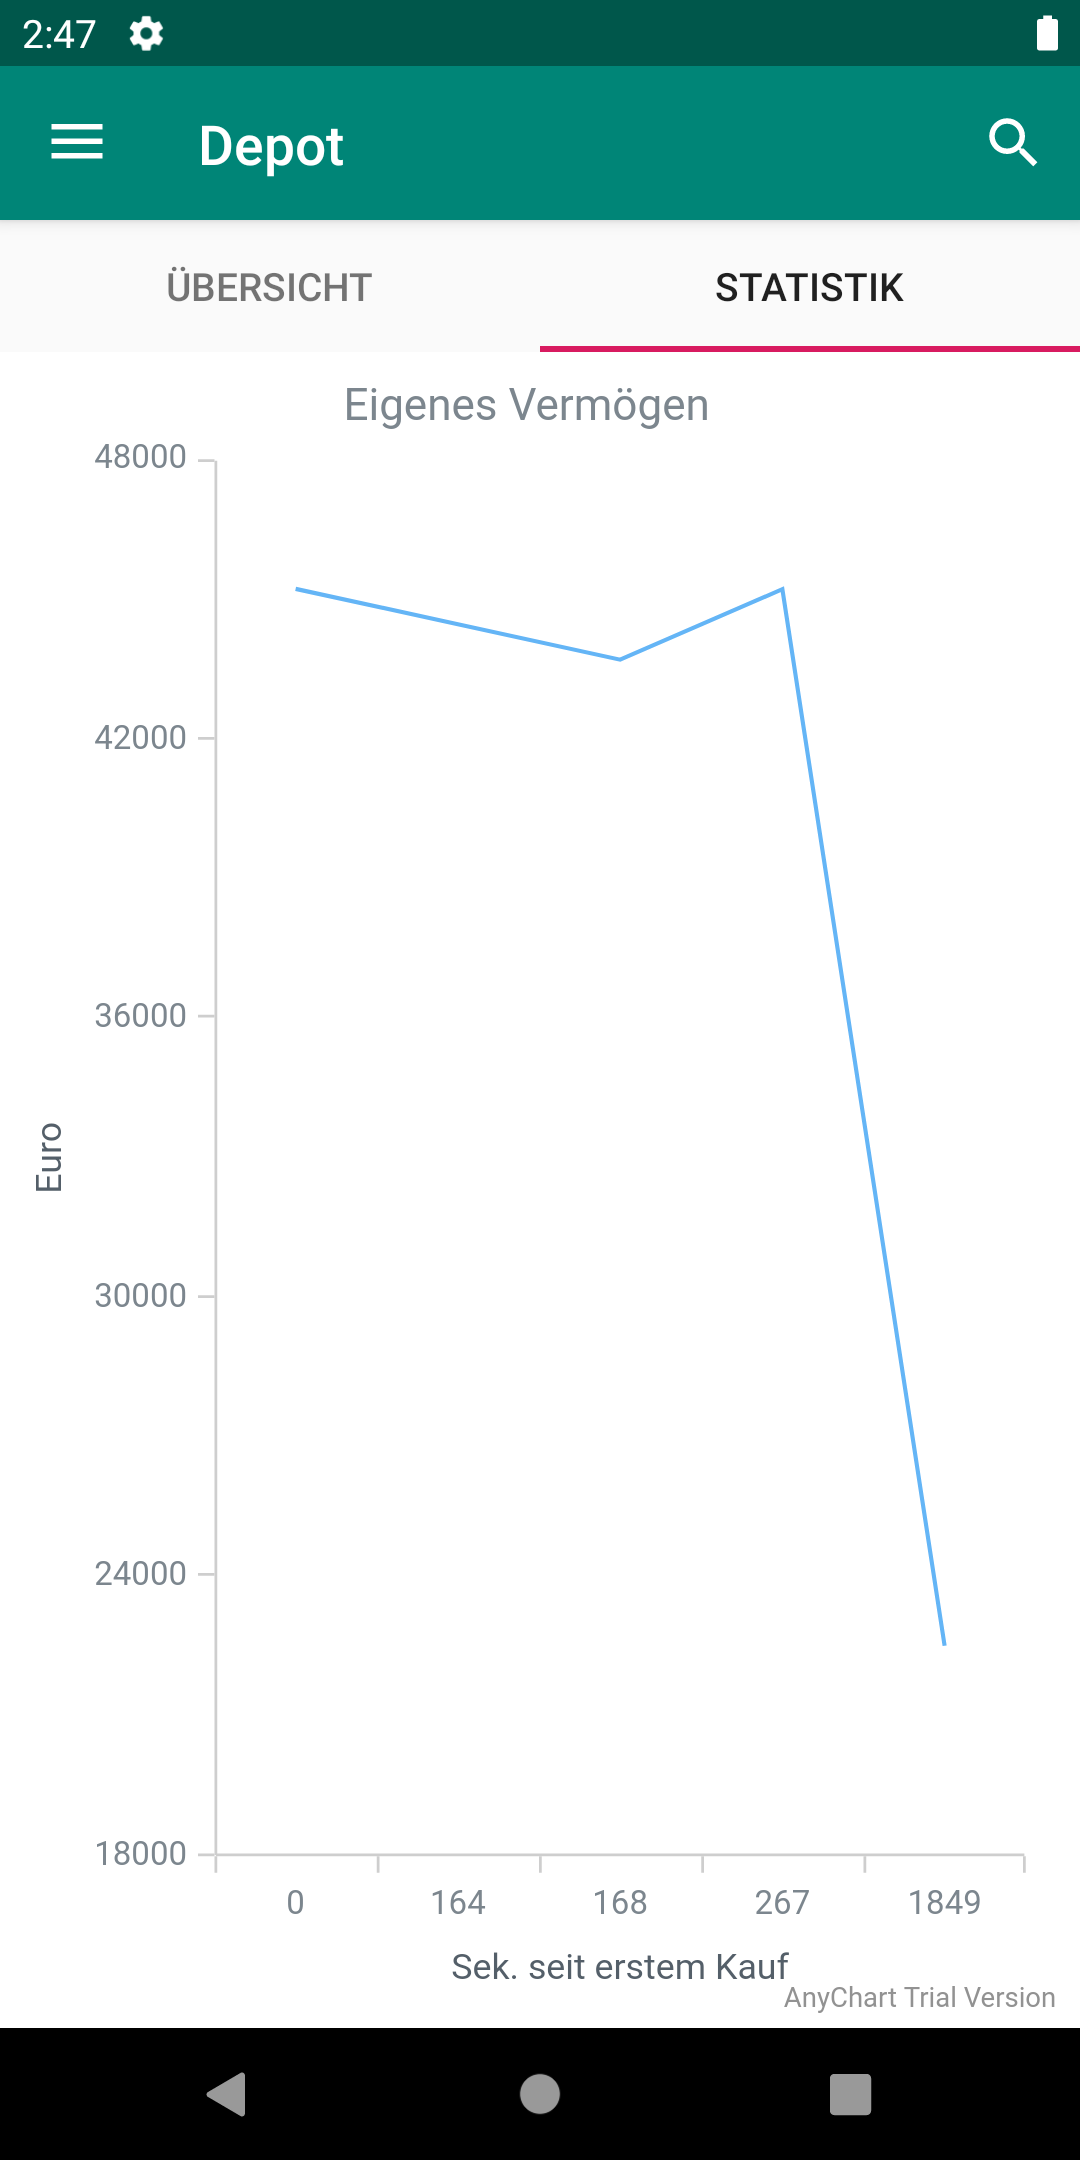
\includegraphics[width=0.6\textwidth]{Bilder/Prsi/verlauf.png}
	\caption{Gefüllte Statistik mit Beispielwerten}
\end{figure}


\subsubsection{Transaktionskosten}

Die Transaktionskosten sind in der Application im Punkt Schwierigkeitsgerade aufgegangen. Dabei wird jetzt nicht nur ein Betrag bei jeder Transaktion der einem Prozentwert des Handels Volumen von dem Geld des Spielers abgezogen, sondern diese Höhe kann auch noch verändert werden. Daher findet sich dieser Eintrag in dem Bereich Zusatzfeatures ebenfalls wieder und zeigt dort sein volles Potential.

\subsubsection{Aktien kaufen/verkaufen(Live Trading)}

Das Kauf System der App Broken Broke Broker kann von jeder Aktienübersicht direkt angesteuert werden. Dadurch wird gezielt eine Aktie gekauft und der Marketineffekt des berührten Produkts genutzt. Der Spieler drückt auf eine Aktie und kann sie erst jetzt kaufen. Im Moment des Tippens baut der Kunde eine taktile Bildung zum Produkt auf und verleitet daher eher zum kaufen. Der Verkauf einer Aktie erfolgt ebenfalls über die Detailsicht der Aktie und kann damit sowohl vom Depot, wie auch von Suche, Historie oder anderen Punkten im Menü aufgerufen zu werden. Dadurch wird die Produktbindung des Spielers gestärkt und ein bewusstes und einfaches Handeln ermöglicht. Der eingeblendete Preis direkt unter dem Chart der Aktie sorft für Übersichtlichkeit des Handeln und schafft Umsicht.

Ansicht von Kaufen und Verkaufen:

\begin{figure}[H]
	\centering
	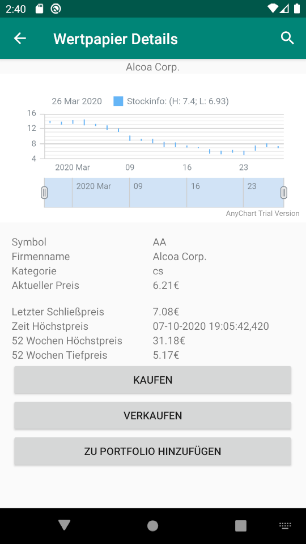
\includegraphics[width=0.6\textwidth]{Bilder/Prsi/detailansicht.png}
	\caption{Detailansicht mit den Buttons Kaufen und Verkaufen}
\end{figure}

\begin{figure}[H]
	\centering
	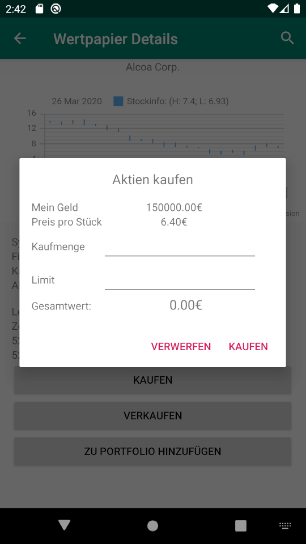
\includegraphics[width=0.6\textwidth]{Bilder/Prsi/Kaufdialog.png}
	\caption{Ansicht des Kauf-/Verkaufdialog}
\end{figure}



\subsubsection{Historie über Käufe und Verkäufe}

In dem Reiter History werden alle vergangenen Traksaktionen anzeigt. Dies schafft einen Überblick darüber welcher Handel in der Vergangenheit gut und welcher schlecht gelaufen ist. Dabei ist hier am wichtigsten, dass die Daten persistent und frei von jeglichen bewertenden Details sind. Grundlage für diese Funktion ist ein Virtueller Kassenzettel, der die einzelnen Positionen darstellt und am Ende das entscheidende Ergebnis an den Spieler vermittelt.

\begin{figure}[H]
	\centering
	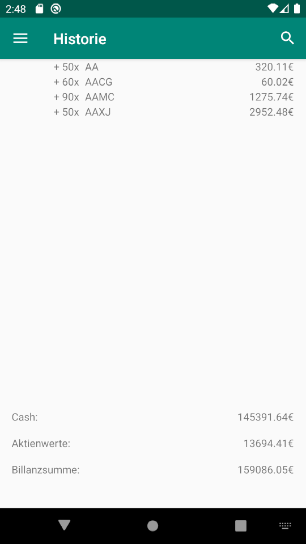
\includegraphics[width=0.6\textwidth]{Bilder/Prsi/kassenzettel.png}
	\caption{Anzeige des Kassenzettels}
\end{figure}

\subsubsection{Automatischer Handel im Hintergrund}

Der Automatisierte Handel im Hintergrund erfolgt in der Application Über einen Worker abgearbeitet. Dieser wird erst mit dem ersten Starten der App gestartet um die Kunden nicht mit Werbemeldungen zu erregen und den Fokus des Spiels auf die Zeit im Spiel zu lenken. Sobald die App einmal gestartet ist, arbeitet sie jedoch nach bekannten Mustern um den Kunden am Spiel zu halten. Pushnachrichten und automatisierter Handel sind von diesem Zeitpunkt aus verfügbar. Die Automatischen Handelspositionen werden nach Los und Call abgearbeitet, wobei beide nach der gleichen Priorität abgearbeitet werden, jedoch Verkäufe vor Verkäufen zeitlich abgearbeitet werden um Verluste zu vermeiden.

\subsubsection{Spiel zurücksetzen / Neustarten}
Der Button um das Spiel zurück zu setzen wirdunter dem Button NewGame gebaut und zeigt dort den aktuellen Kontostand an. Das soll den Nutzer Motivieren das erreichte nicht einfach aufzugeben und sich das zurücksetzen des Spiels gut zu überlegen. Sollte der Spieler doch darauf klicken wird die App zurück auf den Initialen Startwert gesetzt.

\begin{figure}[H]
	\centering
	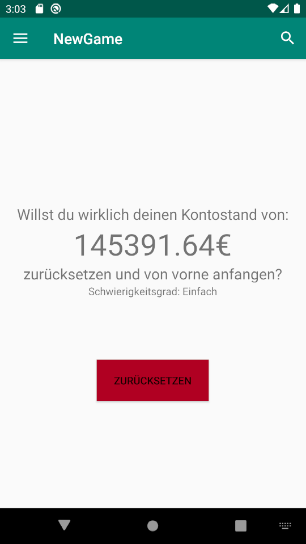
\includegraphics[width=0.6\textwidth]{Bilder/Prsi/newGame.png}
	\caption{Anzeige des Kassenzettels}
\end{figure}

\subsection{Vorstellung der Zusatzfunktionen}
In diesem Abschnitt werden die geforderten Zusatzfunktionen dargestellt. In des Rahmen Seminars wurden folgende Funktionen ausgearbeitet:
	
	
	\subsubsection{Erfolge}
	In der App Broken Broke Broker kann die Schwierigkeitseinstellungen vorgewählt werden. Die Einstellung beschreibt die Fällige Tobinsteuer auf jede Transaktion und das gegebene Startkapital. Wird ein neues Spiel gestartet wird der Wert des Schwierigkeitsgrades neu gesetzt. Der Wert in innerhalb der APP Persistent gehalten.
	\begin{figure}[H]
		\centering
		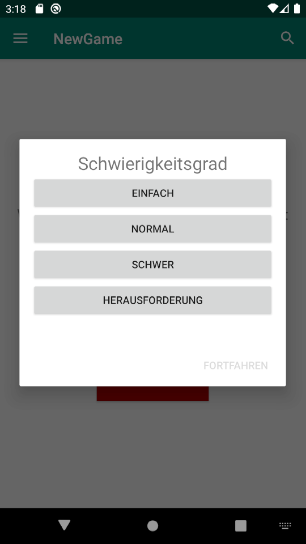
\includegraphics[width=0.6\textwidth]{Bilder/Prsi/diff.png}
		\caption{Anzeige zum Wählen des Schwierigkeitsgrades}
	\end{figure}
	 
	\subsubsection{Detailansicht der Aktien}
	Die Detailansicht der Aktien ist bei uns ein Zentrales Element der App. Hier sieht man alle Details einer Aktie und auch das Diagramm der Aktie. Alles was dem Spieler neugierig macht auf eine unbekannte Aktie an Informationen zu finden ist wichtig.
	
    \begin{figure}[H]
		\centering
		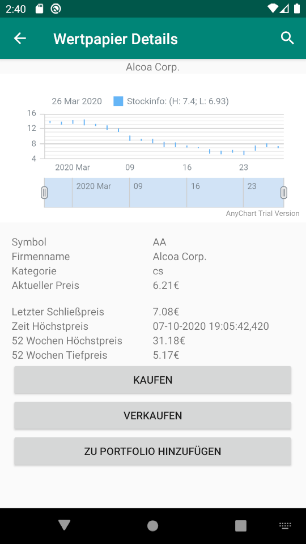
\includegraphics[width=0.6\textwidth]{Bilder/Prsi/detailansicht.png}
		\caption{Anzeige für die Aktienübersicht}
	\end{figure} 
	\newpage
	\subsubsection{Schwierigkeitsgrad Einstellungen}
		Die Einstellung des Schwierigkeitsgrades bringt die App auf ein neues Level und sorgt dafür, dass der erfahrene Broker genauso gefordert wird, wie der einfache Börsenanfänger. Diese Einstellung verändert das Startkapital und die Kosten für den Trade.
		\newline \newline Die Werte sind folgend:\newline Einfach \quad \quad \quad \quad \euro{150.000} \quad \quad 0,035\%\newline Normal \quad \quad \quad \quad \euro{50.000}\quad \quad \quad 0,0125\%\newline Schwierig \quad \quad \quad  \euro{50.000} \quad \quad \quad 0,5\%\newline Herausforderung\quad \euro{1.000}\quad  \quad \quad 0.5\%
	\subsection{Persistenz}
	
	
	
	
\section{Fazit}
%Hier ist wichtig, dass wir es schaffen können zu zeigen, ob wir mit den erreichten Zielen zufrieden sind.

Am Ende eines Projekts wie dem Java Code Camp schaut man zurück und überlegt, was man selbst für die Zukunft aus der Projektarbeit lernen kann. Die App Broken Broke Broker halten wir als Team für eine gelungene Anwendung. Die Zeit, die wir mit dem Code verbringen mussten war immens hoch, da wir Anfangs die Technologie-entscheidung für Java getroffen hatten. Diese hat uns im folgenden viel Kraft gekostet. Letztlich haben wir aber eine App auf den Markt gebracht, die den Kriterien der Anforderungen entspricht. Wir würden uns für das nächste Projekt dieser Art im Fachbereich wünschen, dass wir die Technologie vielleicht etwas enger vorgegeben bekommen, damit uns eine strategische Fehlentscheidung nicht mehr in dieser Art beschneidet.

\newpage
%\renewcommand{\listoffigures}{Bildverzeichnis}
\listoffigures



\end{document}
